%%%%%%%%%%%%%%%%%%%%%%%%%%%%%%%%%%%%%%
% ATTTENTION
% compile with ps->pdf!
%%%%%%%%%%%%%%%%%%%%%%%%%%%%%%%%%%%%%%

\documentclass[a4paper,twocolumn,10pt,fleqn]{book}
\usepackage[american,ngerman]{babel}     %american / ngerman
\usepackage[OT1]{fontenc}       %Silbentrennung
\usepackage[utf8]{inputenc}
%\usepackage[latin1]{inputenc}  %Direkteingabe von Umlauten
\usepackage{tabularx}
\usepackage{multirow}
\usepackage{colortbl}
\usepackage{longtable}
\usepackage{supertabular}
\usepackage{graphicx}
\usepackage{times}       %Erzwingt Typ 1 Schrift (skalierbar, gutes pdf-Output)
\usepackage[round,colon,authoryear]{natbib}      %Fuer Zitate mit \citep, \citet
\usepackage[fleqn]{amsmath}  % für \align-environment (ausgerichtete Gleichungen)
\usepackage{wasysym}  % common symbols (math + text mode), e.g. \permil
\usepackage{fancyhdr} % Customized header/footer
\usepackage{titling}
\usepackage{fink}
\usepackage{listings}
\usepackage{xcolor}
\usepackage{framed}
\usepackage{amsmath}
\usepackage[hyphens,obeyspaces]{url}
\usepackage{datatool}
\usepackage{lscape}
\usepackage{seqsplit} % automatically split very long sequences of letters or numbers; use: \seqsplit{[...]}
\usepackage[mode=text,exponent-product = \cdot]{siunitx} % display numbers and si units
\sisetup{locale=UK}


%Unterdrueckung von Hurenkindern und Schusterjungen
\clubpenalty = 10000
\widowpenalty = 10000 \displaywidowpenalty = 10000

% Vertiacal spacing between multi-line equations (e.g. in align env.)
\setlength{\jot}{11pt}

\newcommand{\fmtClassDesc}[1]{\usefont{OT1}{phv}{mc}{n} \fontsize{8pt}{8pt}
  \selectfont #1}

\newcommand{\ECHSEENGINES}{../../echse_engines}


  
%%%%%%%%%%%%%%%%%%%%%%%%%%%%%%%%%%%%%%%%%%%%%%%%%%%%%%%%%
%%%%%%%%%%%%%%%%%%%%%% DEFINITIONS %%%%%%%%%%%%%%%%%%%%%%
%%%%%%%%%%%%%%%%%%%%%%%%%%%%%%%%%%%%%%%%%%%%%%%%%%%%%%%%%

%%%%%%%%%%%%%%%%%%%%%%%%%%%%%%%%%%%%%%%%%
% Optionen f�r die PDF-Erstellung 
%
% Achtung: Der Postprocessor dvips muss
%   mit der Option -z ausgef�hrt werden.
%%%%%%%%%%%%%%%%%%%%%%%%%%%%%%%%%%%%%%%%%
\usepackage[ps2pdf]{hyperref} % tp: commented this out because this produces an error when using pdflatex for compilation
\usepackage{breakurl}
\definecolor{darkblue}{rgb}{0.2,0.2,0.8}
\hypersetup{%
colorlinks=true,        % Einfaerbung von Verknuepfungen
linkcolor=darkblue,     %Farbe dokumentinterner Links
citecolor=darkblue,     %Farbe dokumentinterner Links
bookmarksopen=false,    % Anzeige aller Ebenen
bookmarksnumbered=true, % Anzeige der Abschnittsnummern
pdfstartpage={1},       % Startseite
breaklinks=true
}

\input{../_common/options-captions}
\input{../_common/options-crossref}
\input{../_common/options-lists}
\input{../_common/options-inputlistings.tex}
\input{../_common/options-hyphen}
\input{../_common/formats}
\input{../_common/abbrev_misc}


%%%%%%%%%%%%%%%%%%%%%%%%%%%%%%%%%%%%%%%%%%%%%%%%%%%%%%%%%%%%%%%%%%%%%%%%%%%%%%%%
% HYDRO-METEOROLOGICAL VARIABLES
%%%%%%%%%%%%%%%%%%%%%%%%%%%%%%%%%%%%%%%%%%%%%%%%%%%%%%%%%%%%%%%%%%%%%%%%%%%%%%%%

% Basic meteorological variables
\newcommand{\precipIntensity}{\ensuremath{PI}}
\newcommand{\windspeed}{\ensuremath{WS}}
\newcommand{\airtemp}{\ensuremath{TA}}
\newcommand{\airtempMin}{\ensuremath{TA_{min}}}
\newcommand{\airtempMax}{\ensuremath{TA_{max}}}
\newcommand{\airPressure}{\ensuremath{PA}}
\newcommand{\relHumidity}{\ensuremath{RH}}
\newcommand{\solarRadiation}{\ensuremath{SR}}
\newcommand{\sundur}{\ensuremath{n}}

% Variables related to moisture / humidity
\newcommand{\specHumidity}{\ensuremath{q}}
\newcommand{\specHumiditySurface}{\ensuremath{q_s}}
\newcommand{\vaporPressure}{\ensuremath{e}}
\newcommand{\vaporPressureSurface}{\ensuremath{e_s}}
\newcommand{\satVaporPressure}{\ensuremath{E}}
\newcommand{\satVaporPressureIce}{\ensuremath{E_i}}
\newcommand{\satVaporPressureWater}{\ensuremath{E_w}}
\newcommand{\vaporPressureDeficit}{\ensuremath{D}}
\newcommand{\vapPresDefCano}{\ensuremath{D_0}}
\newcommand{\slopeSatVapCurve}{\ensuremath{s}}
\newcommand{\psychroConst}{\ensuremath{\gamma}}

% Other meteorological variables
\newcommand{\cloudFraction}{\ensuremath{FC}}
\newcommand{\dewpointTemperature}{\ensuremath{T_{dew}}}
\newcommand{\moleFracWaterVap}{\ensuremath{x_{v}}}
\newcommand{\compressibilityFactor}{\ensuremath{Z}}

% Common (unspecific) hydrometeorological variables
\newcommand{\temperature}{\ensuremath{T}}

% Snow variables
\newcommand{\snowWaterEquivalent}{\ensuremath{SWE}}
\newcommand{\snowHeight}{\ensuremath{SH}}
\newcommand{\snowEnergyContent}{\ensuremath{SEC}}
\newcommand{\snowTemperature}{\ensuremath{T_s}}
\newcommand{\snowSurfaceTemperature}{\ensuremath{T_{ss}}}
\newcommand{\snowFractionLiquid}{\ensuremath{SLF}}
\newcommand{\snowRelSaturation}{\ensuremath{RSS}}

% other
\newcommand{\measHeightTemp}{\ensuremath{z_t}}
\newcommand{\measHeightRelhum}{\ensuremath{z_h}}
\newcommand{\measHeightWind}{\ensuremath{z_w}}



%%%%%%%%%%%%%%%%%%%%%%%%%%%%%%%%%%%%%%%%%%%%%%%%%%%%%%%%%%%%%%%%%%%%%%%%%%%%%%%%
% HYDRO-METEOROLOGICAL PROCESS RATES AND RELATED CONVERSION FACTORS
%%%%%%%%%%%%%%%%%%%%%%%%%%%%%%%%%%%%%%%%%%%%%%%%%%%%%%%%%%%%%%%%%%%%%%%%%%%%%%%%

% Energy fluxes
\newcommand{\netRadiation}{\ensuremath{R_{net}}}
\newcommand{\netRadiationSoil}{\ensuremath{R_{net,soil}}}
\newcommand{\netRadiationShort}{\ensuremath{R_{netS}}}
\newcommand{\netRadiationLong}{\ensuremath{R_{netL}}}
\newcommand{\heatfluxSens}{\ensuremath{H_{sens}}}
\newcommand{\heatfluxSoil}{\ensuremath{G_{soil}}}
\newcommand{\heatfluxVegSoil}{\ensuremath{G_{total}}}

\newcommand{\radLongwaveOut}{\ensuremath{R_{outL}}}
\newcommand{\radLongwaveIn}{\ensuremath{R_{inL}}}
\newcommand{\radLongwaveInClearsky}{\ensuremath{R_{inL,cs}}}
\newcommand{\radLongwaveInClouds}{\ensuremath{R_{inL,cl}}}

\newcommand{\radShortwaveIn}{\ensuremath{R_{inS}}}
\newcommand{\radShortwaveInClearsky}{\ensuremath{R_{inS,cs}}}

\newcommand{\radExtraterr}{\ensuremath{R_{ex}}}
\newcommand{\radExtraterrDaily}{\ensuremath{R_{ex,daily}}}
\newcommand{\radExtraterrHourly}{\ensuremath{R_{ex,hourly}}}

% Mass fluxes
\newcommand{\massfluxPrec}{\ensuremath{M_{prec}}}
\newcommand{\massfluxSubl}{\ensuremath{M_{subl}}}
\newcommand{\massfluxFlow}{\ensuremath{M_{flow}}}

% Evapotranspiration
\newcommand{\et}{\ensuremath{et}}
\newcommand{\etPot}{\ensuremath{et_{pot}}}
\newcommand{\etRef}{\ensuremath{et_{ref}}}
\newcommand{\etRefDaily}{\ensuremath{et_{ref,d}}}
\newcommand{\etRefHourly}{\ensuremath{et_{ref,h}}}
\newcommand{\etReal}{\ensuremath{et_{act}}}
\newcommand{\etTransp}{\ensuremath{et_{c}}}
\newcommand{\etEvap}{\ensuremath{et_{s}}}



%%%%%%%%%%%%%%%%%%%%%%%%%%%%%%%%%%%%%%%%%%%%%%%%%%%%%%%%%%%%%%%%%%%%%%%%%%%%%%%%
% PHYSICAL CONSTANTS AND CONCEPTUAL PARAMETERS USED IN HYDRO-METEOROLOGY
%%%%%%%%%%%%%%%%%%%%%%%%%%%%%%%%%%%%%%%%%%%%%%%%%%%%%%%%%%%%%%%%%%%%%%%%%%%%%%%%

% Densities
\newcommand{\densityWater}{\ensuremath{\rho_{w}}}
\newcommand{\densityIce}{\ensuremath{\rho_{i}}}
\newcommand{\densityAir}{\ensuremath{\rho_{air}}}
\newcommand{\densityAirDry}{\ensuremath{\rho_{air,dry}}}
\newcommand{\densityAirMoist}{\ensuremath{\rho_{air}}}
\newcommand{\densitySnow}{\ensuremath{\rho_{snow}}}
\newcommand{\densitySnowDry}{\ensuremath{\rho_{snow,dry}}}
\newcommand{\densitySoil}{\ensuremath{\rho_s}}

% Molar constants
\newcommand{\molMassDryAir}{\ensuremath{M_{a}}}
\newcommand{\molMassWater}{\ensuremath{M_{w}}}
\newcommand{\molGasConst}{\ensuremath{R}}

% Specific heat capacities
\newcommand{\specHeatWater}{\ensuremath{C_{wat}}}
\newcommand{\specHeatIce}{\ensuremath{C_{ice}}}
\newcommand{\specHeatAir}{\ensuremath{C_{air}}}
\newcommand{\specHeatSoil}{\ensuremath{C_s}}

% Latent heats
\newcommand{\evapHeatWater}{\ensuremath{E_{wat}}}
\newcommand{\evapHeatWaterZero}{\ensuremath{E_{wat,0}}}
\newcommand{\fusionHeatIce}{\ensuremath{H_{ice}}}
\newcommand{\sublimHeatIce}{\ensuremath{E_{ice}}}

% Radiation
\newcommand{\snowAlbedo}{\ensuremath{AS}}
\newcommand{\snowAlbedoMin}{\ensuremath{AS_{min}}}
\newcommand{\snowAlbedoMax}{\ensuremath{AS_{max}}}
\newcommand{\snowAlbedoRng}{\ensuremath{AS_{rng}}}

\newcommand{\stefanBoltzmann}{\ensuremath{\sigma}}
\newcommand{\emissivity}{\ensuremath{\varepsilon}}
\newcommand{\cloudCorrFac}{\ensuremath{f}}

\newcommand{\emisa}{\ensuremath{\varepsilon_a}}
\newcommand{\emisb}{\ensuremath{\varepsilon_b}}
\newcommand{\cloudCorrFacA}{\ensuremath{f_a}}
\newcommand{\cloudCorrFacB}{\ensuremath{f_b}}
\newcommand{\angstA}{\ensuremath{a_s}}
\newcommand{\angstB}{\ensuremath{b_s}}
\newcommand{\soilheatDay}{\ensuremath{c_d}}
\newcommand{\soilheatNight}{\ensuremath{c_n}}

\newcommand{\solarConstant}{\ensuremath{R_{SC}}}

% Stoichiometry factors and functions used in the snow model
\newcommand{\stoifacPrecMassToEnergy}{\ensuremath{f_{prec}}}
\newcommand{\stoifacSublMassToEnergy}{\ensuremath{f_{subl}}}
\newcommand{\stoifacFlowMassToEnergy}{\ensuremath{f_{flow}}}

% Various parameters of the snow model
\newcommand{\turbTransCoeff}{\ensuremath{D}}
\newcommand{\airtempRainSnow}{\ensuremath{T_{crit}}}
\newcommand{\soilInteractionDepth}{\ensuremath{D_s}}
\newcommand{\snowRelCapRetent}{\ensuremath{SCR}}
\newcommand{\snowSatHydrCond}{\ensuremath{k_{sat,snow}}}
\newcommand{\snowAlbedoDecrConst}{\ensuremath{k_{AS}}}
\newcommand{\leafAreaIndexFullShadow}{\ensuremath{LAI_{r0}}}

% Turbulence
\newcommand{\karmanConst}{\ensuremath{\kappa}}
\newcommand{\heightDisplace}{\ensuremath{d}}
\newcommand{\roughLenSen}{\ensuremath{z_{om}}}
\newcommand{\roughLenLat}{\ensuremath{z_{ov}}}

% Resistances to evapotranspiration
\newcommand{\resCanopy}{\ensuremath{r_{cs}}}
\newcommand{\resCA}{\ensuremath{r_{ca}}}
\newcommand{\resSoil}{\ensuremath{r_{ss}}}
\newcommand{\resSA}{\ensuremath{r_{sa}}}
\newcommand{\resAero}{\ensuremath{r_{aa}}}
\newcommand{\resLeafAct}{\ensuremath{r_{l,act}}}

\newcommand{\condStress}{\ensuremath{\Phi_{stress}}}
\newcommand{\condSoilWat}{\ensuremath{\Phi_{wat}}}
\newcommand{\condVapPress}{\ensuremath{\Phi_{vap}}}
\newcommand{\condVapPressPar}{\ensuremath{a_{vap}}}

% Land-cover parameters
\newcommand{\cropfacMak}{\ensuremath{c_{Makk}}}
\newcommand{\cropfacFAO}{\ensuremath{c_{FAO}}}
\newcommand{\canoHeight}{\ensuremath{h_{cano}}}
\newcommand{\leafAreaIndex}{\ensuremath{LAI}}
\newcommand{\albedoChangeRate}{\ensuremath{G_{alb}}}
\newcommand{\albedo}{\ensuremath{\mu}}
\newcommand{\canoExt}{\ensuremath{\epsilon}}
\newcommand{\resLeafMin}{\ensuremath{r_{l,min}}}
\newcommand{\radShortHalf}{\ensuremath{g_{srad}}}
\newcommand{\resMeanBound}{\ensuremath{r_{b}}}
\newcommand{\dragCoef}{\ensuremath{c_{d}}}
\newcommand{\roughSoil}{\ensuremath{z_{r,s}}}
\newcommand{\eddyDecay}{\ensuremath{n}}
\newcommand{\rssa}{\ensuremath{k_{rss,a}}}
\newcommand{\rssb}{\ensuremath{k_{rss,b}}}




%%%%%%%%%%%%%%%%%%%%%%%%%%%%%%%%%%%%%%%%%%%%%%%%%%%%%%%%%%%%%%%%%%%%%%%%%%%%%%%%
% ASTRONOMICAL PARAMETERS
%%%%%%%%%%%%%%%%%%%%%%%%%%%%%%%%%%%%%%%%%%%%%%%%%%%%%%%%%%%%%%%%%%%%%%%%%%%%%%%%

\newcommand{\solDecl}{\ensuremath{\delta}}
\newcommand{\eccCorr}{\ensuremath{E_{0}}}
\newcommand{\dayTimeFac}{\ensuremath{\omega_{s}}}
\newcommand{\doy}{\ensuremath{doy}}
\newcommand{\hour}{\ensuremath{h}}
\newcommand{\utcAdd}{\ensuremath{a_{UTC}}}
\newcommand{\lat}{\ensuremath{\varphi}}
\newcommand{\lon}{\ensuremath{L_m}}



%%%%%%%%%%%%%%%%%%%%%%%%%%%%%%%%%%%%%%%%%%%%%%%%%%%%%%%%%%%%%%%%%%%%%%%%%%%%%%%%
% CONSTANTS AND VARIABLES RELATED TO RUNOFF GENERATION AND -CONCENTRATION
%%%%%%%%%%%%%%%%%%%%%%%%%%%%%%%%%%%%%%%%%%%%%%%%%%%%%%%%%%%%%%%%%%%%%%%%%%%%%%%%

\newcommand{\soilWaterContent}{\ensuremath{\theta}}
\newcommand{\soilWaterContentMax}{\ensuremath{\theta_{max}}}

\newcommand{\relSat}{\ensuremath{S}}
\newcommand{\relSatInter}{\ensuremath{S_{int}}}
\newcommand{\relSatBase}{\ensuremath{S_{base}}}


\newcommand{\heightRunoffDirect}{\ensuremath{h_{d}}}

\newcommand{\rateRunoffSurf}{\ensuremath{r_{surf}}}
\newcommand{\rateRunoffPref}{\ensuremath{r_{pref}}}
\newcommand{\rateRunoffInter}{\ensuremath{r_{int}}}
\newcommand{\rateRunoffBase}{\ensuremath{r_{base}}}
\newcommand{\rateEvapotransp}{\ensuremath{r_{evap}}}
\newcommand{\rateSnowMelt}{\ensuremath{r_{melt}}}

\newcommand{\soilDepth}{\ensuremath{D}}
\newcommand{\horDepth}{\ensuremath{D_{hor}}}
\newcommand{\satFrac}{\ensuremath{f_{sat}}}
\newcommand{\expSatFrac}{\ensuremath{{\beta}}}

\newcommand{\thresholdSurf}{\ensuremath{{thr_{surf}}}}

\newcommand{\rateWaterSupply}{\ensuremath{WS}}

\newcommand{\expInter}{\ensuremath{{E_{int}}}}
\newcommand{\expBase}{\ensuremath{{E_{base}}}}

\newcommand{\facInter}{\ensuremath{{b_{int}}}}
\newcommand{\facBase}{\ensuremath{{b_{base}}}}

\newcommand{\strSurf}{\ensuremath{{S_{surf}}}}
\newcommand{\strPref}{\ensuremath{{S_{pref}}}}
\newcommand{\strInter}{\ensuremath{{S_{inter}}}}
\newcommand{\strBase}{\ensuremath{{S_{base}}}}

\newcommand{\concTimeIndex}{\ensuremath{{CTI}}}

\newcommand{\satHydrCond}{\ensuremath{k_{f}}}
\newcommand{\hydrCond}{\ensuremath{k_{u}}}

\newcommand{\percol}{\ensuremath{q_{perc}}}
\newcommand{\latflow}{\ensuremath{q_{lat}}}



%%%%%%%%%%%%%%%%%%%%%%%%%%%%%%%%%%%%%%%%%%%%%%%%%%%%%%%%%%%%%%%%%%%%%%%%%%%%%%%%
% SOIL RELATED PARAMETES AND VARIABLES
%%%%%%%%%%%%%%%%%%%%%%%%%%%%%%%%%%%%%%%%%%%%%%%%%%%%%%%%%%%%%%%%%%%%%%%%%%%%%%%%

\newcommand{\capilSuc}{\ensuremath{\psi}}

\newcommand{\sucStressMin}{\ensuremath{\psi_{s,min}}}
\newcommand{\sucStressMax}{\ensuremath{\psi_{s,max}}}

\newcommand{\capilSucWetfront}{\ensuremath{\psi_f}}

\newcommand{\bubblePress}{\ensuremath{h_b}}
\newcommand{\PoresInd}{\ensuremath{\lambda}}

\newcommand{\porosRefill}{\ensuremath{n_r}}

\newcommand{\sorptivity}{\ensuremath{S}}

\newcommand{\waterCont}{\ensuremath{\theta}}
\newcommand{\waterContRoot}{\ensuremath{\theta_{root}}}
\newcommand{\waterContTop}{\ensuremath{\theta_{top}}}
\newcommand{\waterContGrav}{\ensuremath{\theta_{g}}}
\newcommand{\waterContRes}{\ensuremath{\theta_r}}
\newcommand{\waterContSat}{\ensuremath{\theta_s}}
\newcommand{\waterContPwp}{\ensuremath{\theta_{pwp}}}
\newcommand{\waterContFK}{\ensuremath{\theta_{fc}}}
\newcommand{\waterContEtmax}{\ensuremath{\theta_{etmax}}}

\input{../_common/abbrev_units}
\input{../_common/colors}

\addtolength{\evensidemargin}{-1cm}
\addtolength{\oddsidemargin}{+1cm}

\setcounter{tocdepth}{2}     % Numbers up to 0.0.0 in TOC     (chapter= 0, section= 1, subsection= 2 ...)
\setcounter{secnumdepth}{3}  % Numbers up to 0.0.0.0 in text  (chapter= 0, section= 1, subsection= 2 ...)

\arrayrulecolor{black}

\begin{document}

%%%%%%%%%%%%%%%%%%%%%%%%%%%%%%%%%%%%%%%%%%%%%%%%%%%%%%%%%
%%%%%%%%%%%%%%%%%%%%%% TITLE PAGES %%%%%%%%%%%%%%%%%%%%%%
%%%%%%%%%%%%%%%%%%%%%%%%%%%%%%%%%%%%%%%%%%%%%%%%%%%%%%%%%

\selectlanguage{american}
\pagestyle{empty}
\onecolumn

\begin{center}
  \vspace*{5cm}
  \LARGE
  \textbf{Eco-Hydrological Simulation Environment \\ (\software{echse})} \\
  \vspace*{1.2cm}
  Documentation of model engines \\
  \vspace*{2.0cm}
  \includegraphics[width=0.1\textwidth,angle=270]{../_common/fig/logo.eps}
\end{center}

\cleardoublepage

\vspace*{4cm}

\textbf{Developer:}\\
\vspace*{2ex}

\begin{tabular}{ll}
Author      & David Kneis \\
Affiliation & Institute of Earth and Environmental Sciences \\
            & Geo-Ecology Section, \\
            & University of Potsdam, Germany \\
Contact     & david.kneis@uni-potsdam.de \\
            & \\
Project     & PROGRESS \\
Sub-project & D2.2 \\
Funding     & German Ministry of Education and Research (BMBF) \\
\end{tabular}

\vspace*{2cm}

\textbf{Contributor(s):}\\
\vspace*{2ex}

\begin{tabular}{ll}
Author      & Tobias Pilz \\
Affiliation & Institute of Earth and Environmental Science \\
            & University of Potsdam, Germany \\
Contact     & tpilz@uni-potsdam.de \\
            & \\
Funding     & GeoSim (Helmholtz graduate school) \\
            & \\
Contributions & Added \chapref{chap:meteo}, re-formatted and extended \chapref{chap:et} \\
\end{tabular}

\vspace*{2cm}

\begin{tabular}{ll}
Last update & \today{} \\
\end{tabular}

\cleardoublepage

%%%%%%%%%%%%%%%%%%%%%%%%%%%%%%%%%%%%%%%%%%%%%%%%%%%%%%%%%%
%%%%%%%%%%%%%%%%%%%%%% Page style   %%%%%%%%%%%%%%%%%%%%%%
%%%%%%%%%%%%%%%%%%%%%%%%%%%%%%%%%%%%%%%%%%%%%%%%%%%%%%%%%%

%%% Begin Fancy Header Settings
\pagestyle{fancy}                       % Sets fancy header and footer
\fancyfoot{}                            % Delete current footer settings
\renewcommand{\chaptermark}[1]{         % Lower Case Chapter marker style
  \markboth{\chaptername\ \thechapter\ \hspace{0.5cm} #1}{}}
\renewcommand{\sectionmark}[1]{         % Lower case Section marker style
  \markright{\thesection\ \hspace{0.5cm} #1}}
\fancyhead[LE,RO]{\bfseries\thepage}    % Page number (boldface) in left on even pages and right on odd pages
\fancyhead[RE]{\bfseries\leftmark}      % Chapter in the right on even pages
\fancyhead[LO]{\bfseries\rightmark}     % Section in the left on odd pages
\renewcommand{\headrulewidth}{0.3pt}    % Width of head rule %%% Clear Header
%% End Fancy Header Settings

%%%%%%%%%%%%%%%%%%%%%%%%%%%%%%%%%%%%%%%%%%%%%%%%%%%%%%%%%%
%%%%%%%%%%%%%%%%%%%%%% TOC          %%%%%%%%%%%%%%%%%%%%%%
%%%%%%%%%%%%%%%%%%%%%%%%%%%%%%%%%%%%%%%%%%%%%%%%%%%%%%%%%%

%% Begin TOC Settings
\pdfbookmark[1]{\contentsname}{toc}
\fancyhead[LE,RO]{\bfseries\thepage}
\fancyhead[RE]{\bfseries Contents}
\fancyhead[LO]{\bfseries Contents}
\tableofcontents
%% End TOC Settings

%%%%%%%%%%%%%%%%%%%%%%%%%%%%%%%%%%%%%%%%%%%%%%%%%%%%%%%%%%
%%%%%%%%%%%%%%%%%%%%%% THE CHAPTERS %%%%%%%%%%%%%%%%%%%%%%
%%%%%%%%%%%%%%%%%%%%%%%%%%%%%%%%%%%%%%%%%%%%%%%%%%%%%%%%%%

% Reestablish header
\fancyhead[LE,RO]{\bfseries\thepage}    % Page number (boldface) in left on even pages and right on odd pages
\fancyhead[RE]{\bfseries\leftmark}      % Chapter in the right on even pages
\fancyhead[LO]{\bfseries\rightmark}     % Section in the left on odd pages


%%%%% Chapter sources

\onecolumn
\include{chapters/intro/intro}

\twocolumn
\part{Hydrological model engines} \label{part:modelEngines}
\include{chapters/part_modelEngines/hypsoRR/hypsoRR}

\onecolumn
\part{Classes} \label{part:classes}
\chapter{Classes for hydrological catchment modeling} \label{chap:classes:catchmod}

%NOTE: This code is required by the datatool package to make the reading of TAB-separated text files actually work
\catcode`\^^I=12 %
\DTLsetseparator{	}%

% Generate a long table listing all data members
%
% Arg 1: A name for the data base (e.g. use the class' name)
% Arg 2: The data file listing the members
% Arg 3: The table caption
% Arg 4: The label string
\newcommand{\tableOfMembers}[4]{%
\DTLloadrawdb{#1}{#2}
%\begin{landscape}
\begin{center}
\begin{longtable}{llll}
%\begin{tabular}{llll} \\
\caption{#3 \label{#4}} \\
\hline
\fmtClassDesc\bfseries Type & \fmtClassDesc\bfseries Name & \fmtClassDesc\bfseries Description & \fmtClassDesc\bfseries Unit\\
\hline
\endfirsthead
\multicolumn{4}{c}%
{\tablename\ \thetable\ -- \textit{Continued from previous page}} \\
\hline
\fmtClassDesc\bfseries Type & \fmtClassDesc\bfseries Name & \fmtClassDesc\bfseries Description & \fmtClassDesc\bfseries Unit\\
\hline
\endhead
\hline \multicolumn{4}{r}{\textit{Continued on next page}} \\
\endfoot
\hline
\endlastfoot
\DTLforeach{#1}
{\membertype=type,\membername=name,\memberdescr=description,\memberunit=unit}
{%
  \DTLiffirstrow{}{\\}%
  \fmtClassDesc \membertype & \fmtClassDesc \membername & \fmtClassDesc \memberdescr & \fmtClassDesc \memberunit%
}%
\end{longtable}
%\end{tabular}
\end{center}
}

%%%%%%%%%%%%%%%%%%%%%%%%%%%%%%%%%%%%%%%%%%%%%%%%%%%%%%%%%%%%%%%%%%%%%%%%%%%%%%%%%%%%%%%%%%%%%%
%%%%%%%%%%%%%%%%%%%%%%%%%%%%%%%%%%%%%%%%%%%%%%%%%%%%%%%%%%%%%%%%%%%%%%%%%%%%%%%%%%%%%%%%%%%%%%

\section{Default sub-basin class} \label{sec:classes:catchmod:subbasin-default}

\subsection{Simulated processes} \label{sec:classes:catchmod:subbasin-default:processes}
The class simulates the processes listed in \tabref{tab:classes:catchmod:subbasin-default:processes}.

\begin{table}
  \caption{Considered processes in the default sub-basin class. \label{tab:classes:catchmod:subbasin-default:processes}}
\begin{tabular}{|p{0.28\textwidth}p{0.7\textwidth}|} \hline
  \rowcolor[gray]{0.9}
  Process & Model concept \\ \hline
  Runoff generation & Conceptual four components model (\secref{sec:runGen4comp}) \\
  Runoff concentration & Parallel linear reservoirs (\secref{sec:runConcParStor}) \\
  Evapotranspiration & Potential evapotranspiration after Makkink with crop factors and correction for soil water limitation (\secsref{sec:et:makkink}, \ref{sec:eta:cropfactors}, and \ref{sec:eta:soilmoisture}) \\
  Snow storage and melt & Energy balance model (\secref{sec:snow-enBal}) \\
  \hline
\end{tabular}
\end{table}

The current version of the class does \emph{not} allow for the representation of hydrological response units. Only three classes of land cover are currently distinguished: (1) water surfaces, (2) impervious surfaces, and (3) pervious surfaces, \ie{} soil typically covered by vegetation.

\subsection{Data members} \label{sec:classes:catchmod:subbasin-default:members}
A full list of the data members of the class is provided in \tabref{tab:classes:catchmod:subbasin-default:members}. See \citet{Echse-Main-Doc} for an explanation of the abbreviations in the 'type' column.

\begin{landscape}
\tableOfMembers{subbasin-default}{\ECHSEENGINES/classes/declaration/cat_hypsoRR.txt}{Data members of the default sub-basin class.}{tab:classes:catchmod:subbasin-default:members}
\end{landscape}

%%%%%%%%%%%%%%%%%%%%%%%%%%%%%%%%%%%%%%%%%%%%%%%%%%%%%%%%%%%%%%%%%%%%%%%%%%%%%%%%%%%%%%%%%%%%%%
%%%%%%%%%%%%%%%%%%%%%%%%%%%%%%%%%%%%%%%%%%%%%%%%%%%%%%%%%%%%%%%%%%%%%%%%%%%%%%%%%%%%%%%%%%%%%%

\section{Default reach class} \label{sec:classes:catchmod:reach-default}

\subsection{Simulated processes} \label{sec:classes:catchmod:reach-default:processes}
The reach class simulates the outflow from a river reach given information on the inflow and its storage characteristics. The concept is described in \secref{sec:chanFlow_singleRes}.

\subsection{Data members} \label{sec:classes:catchmod:reach-default:members}
A list of the data members of the class is provided in \tabref{tab:classes:catchmod:reach-default:members}. See \citet{Echse-Main-Doc} for an explanation of the abbreviations in the 'type' column.

%\begin{landscape}
\tableOfMembers{reach-default}{\ECHSEENGINES/classes/declaration/rch.txt}{Data members of the default reach class.}{tab:classes:catchmod:reach-default:members}
%\end{landscape}

%%%%%%%%%%%%%%%%%%%%%%%%%%%%%%%%%%%%%%%%%%%%%%%%%%%%%%%%%%%%%%%%%%%%%%%%%%%%%%%%%%%%%%%%%%%%%%
%%%%%%%%%%%%%%%%%%%%%%%%%%%%%%%%%%%%%%%%%%%%%%%%%%%%%%%%%%%%%%%%%%%%%%%%%%%%%%%%%%%%%%%%%%%%%%

\section{Minireach class} \label{sec:classes:catchmod:minireach}

\subsection{Simulated processes} \label{sec:classes:catchmod:minireach:processes}
The minireach class simulates a reach (or pipe) of very short length so that the travel time is practically negligible. Thus, the outflow a minireach object is identical to the inflow.

\subsection{Data members} \label{sec:classes:catchmod:minireach:members}
A list of the data members of the class is provided in \tabref{tab:classes:catchmod:minireach:members}. See \citet{Echse-Main-Doc} for an explanation of the abbreviations in the 'type' column.

%\begin{landscape}
\tableOfMembers{minireach}{\ECHSEENGINES/classes/declaration/minirch.txt}{Data members of the minireach class.}{tab:classes:catchmod:minireach:members}
%\end{landscape}

%%%%%%%%%%%%%%%%%%%%%%%%%%%%%%%%%%%%%%%%%%%%%%%%%%%%%%%%%%%%%%%%%%%%%%%%%%%%%%%%%%%%%%%%%%%%%%
%%%%%%%%%%%%%%%%%%%%%%%%%%%%%%%%%%%%%%%%%%%%%%%%%%%%%%%%%%%%%%%%%%%%%%%%%%%%%%%%%%%%%%%%%%%%%%

\section{Node classes} \label{sec:classes:catchmod:nodes}

\subsection{Simulated processes} \label{sec:classes:catchmod:nodes:processes}
The purpose of node objects is to merge flows from different sources. The typical case is a node with two inflows (\eg{} a stream junction). Nodes with a higher numbner of inflows (or with just a single inflow) may be useful in some situations.

\subsection{Data members} \label{sec:classes:catchmod:nodes:members}
A list of the data members of the class is provided in \tabref{tab:classes:catchmod:nodes:members} for the example of two inflows. See \citet{Echse-Main-Doc} for an explanation of the abbreviations in the 'type' column.

%\begin{landscape}
\tableOfMembers{node}{\ECHSEENGINES/classes/declaration/node_n2.txt}{Data members of the node class with two inflows.}{tab:classes:catchmod:nodes:members}
%\end{landscape}

%%%%%%%%%%%%%%%%%%%%%%%%%%%%%%%%%%%%%%%%%%%%%%%%%%%%%%%%%%%%%%%%%%%%%%%%%%%%%%%%%%%%%%%%%%%%%%
%%%%%%%%%%%%%%%%%%%%%%%%%%%%%%%%%%%%%%%%%%%%%%%%%%%%%%%%%%%%%%%%%%%%%%%%%%%%%%%%%%%%%%%%%%%%%%

\section{Lake class} \label{sec:classes:catchmod:lake}

\subsection{Simulated processes} \label{sec:classes:catchmod:lake:processes}
The class simulates the outflow from an uncontrolled lake/reservoir based on a rating curve and a storage curve. Precipitation and evaporation losses are taken into account. Details are described in \secref{sec:resStor_lake}.

\subsection{Data members} \label{sec:classes:catchmod:lake:members}
A list of the data members of the class is provided in \tabref{tab:classes:catchmod:lake:members}. See \citet{Echse-Main-Doc} for an explanation of the abbreviations in the 'type' column.

%\begin{landscape}
\tableOfMembers{lake}{\ECHSEENGINES/classes/declaration/lake.txt}{Data members of the lake class.}{tab:classes:catchmod:lake:members}
%\end{landscape}

%%%%%%%%%%%%%%%%%%%%%%%%%%%%%%%%%%%%%%%%%%%%%%%%%%%%%%%%%%%%%%%%%%%%%%%%%%%%%%%%%%%%%%%%%%%%%%
%%%%%%%%%%%%%%%%%%%%%%%%%%%%%%%%%%%%%%%%%%%%%%%%%%%%%%%%%%%%%%%%%%%%%%%%%%%%%%%%%%%%%%%%%%%%%%

\section{Gage class} \label{sec:classes:catchmod:gage}

\subsection{Simulated processes} \label{sec:classes:catchmod:gage:processes}
In many situations it is sufficient to output the simulated flow rate of a river reach, making the explicit simulation of a gage object unnecessary. The advantage of instantiating an object of the gage class lies in the fact that the simulated flow may be optionally substituted by observed values. This is quite useful, for example, when a calibrating a model for the part of a river basins located downstream of a gage.

\subsection{Data members} \label{sec:classes:catchmod:gage:members}
A list of the data members of the class is provided in \tabref{tab:classes:catchmod:gage:members}. See \citet{Echse-Main-Doc} for an explanation of the abbreviations in the 'type' column.

%\begin{landscape}
\tableOfMembers{gage}{\ECHSEENGINES/classes/declaration/gage.txt}{Data members of the gage class.}{tab:classes:catchmod:gage:members}
%\end{landscape}

%%%%%%%%%%%%%%%%%%%%%%%%%%%%%%%%%%%%%%%%%%%%%%%%%%%%%%%%%%%%%%%%%%%%%%%%%%%%%%%%%%%%%%%%%%%%%%
%%%%%%%%%%%%%%%%%%%%%%%%%%%%%%%%%%%%%%%%%%%%%%%%%%%%%%%%%%%%%%%%%%%%%%%%%%%%%%%%%%%%%%%%%%%%%%

\section{Rain gage class} \label{sec:classes:catchmod:raingage}

\subsection{Simulated processes} \label{sec:classes:catchmod:raingage:processes}
Objects of this class can be used to query the precipitation at a point as computed from residual interpolation.

\subsection{Data members} \label{sec:classes:catchmod:raingage:members}
A list of the data members of the class is provided in \tabref{tab:classes:catchmod:raingage:members}. See \citet{Echse-Main-Doc} for an explanation of the abbreviations in the 'type' column.

%\begin{landscape}
\tableOfMembers{raingage}{\ECHSEENGINES/classes/declaration/raingage.txt}{Data members of the rain gage class.}{tab:classes:catchmod:raingage:members}
%\end{landscape}

%%%%%%%%%%%%%%%%%%%%%%%%%%%%%%%%%%%%%%%%%%%%%%%%%%%%%%%%%%%%%%%%%%%%%%%%%%%%%%%%%%%%%%%%%%%%%%
%%%%%%%%%%%%%%%%%%%%%%%%%%%%%%%%%%%%%%%%%%%%%%%%%%%%%%%%%%%%%%%%%%%%%%%%%%%%%%%%%%%%%%%%%%%%%%

\section{External inflow class} \label{sec:classes:catchmod:ext-inflow}

\subsection{Simulated processes} \label{sec:classes:catchmod:ext-inflow:processes}
This class provides a simple means to represent an external water source. The time-variable flow rates are pre-defined, \ie{} read from a file. The class may also be helpful if a large-scale model is split into sub-models at the boundaries of major watersheds. In such a case, it may be desireable to save the runoff from an upstream area (sub-model A) to a file and re-read the data later when simulating the downstream part (sub-model B).

\subsection{Data members} \label{sec:classes:catchmod:ext-inflow:members}
A list of the data members of the class is provided in \tabref{tab:classes:catchmod:ext-inflow:members}. See \citet{Echse-Main-Doc} for an explanation of the abbreviations in the 'type' column.

%\begin{landscape}
\tableOfMembers{ext-inflow}{\ECHSEENGINES/classes/declaration/raingage.txt}{Data members of the external inflow class.}{tab:classes:catchmod:ext-inflow:members}
%\end{landscape}

%%%%%%%%%%%%%%%%%%%%%%%%%%%%%%%%%%%%%%%%%%%%%%%%%%%%%%%%%%%%%%%%%%%%%%%%%%%%%%%%%%%%%%%%%%%%%%
%%%%%%%%%%%%%%%%%%%%%%%%%%%%%%%%%%%%%%%%%%%%%%%%%%%%%%%%%%%%%%%%%%%%%%%%%%%%%%%%%%%%%%%%%%%%%%

\subsection{Reservoir class}
This class is still experimental and not documented.

%%%%%%%%%%%%%%%%%%%%%%%%%%%%%%%%%%%%%%%%%%%%%%%%%%%%%%%%%%%%%%%%%%%%%%%%%%%%%%%%%%%%%%%%%%%%%%
%%%%%%%%%%%%%%%%%%%%%%%%%%%%%%%%%%%%%%%%%%%%%%%%%%%%%%%%%%%%%%%%%%%%%%%%%%%%%%%%%%%%%%%%%%%%%%

\subsection{Flood control storage basin class}
This class is still experimental and not documented.


\twocolumn
\part{Mathematical description of hydrological processes} \label{part:processes}
\include{chapters/part_processes/snow/snow}
\chapter{Runoff generation} \label{chap:runGen}
\renewcommand{\tabdir}{chapters/part_processes/runoffGeneration/tab}
\renewcommand{\figdir}{chapters/part_processes/runoffGeneration/fig}

\section{Introduction} \label{sec:runGen_intro}

To avoid confusion, it is important to distinguish between the terms \emph{runoff generation} and \emph{runoff concentration}. As \emph{runoff generation}, we understand the transformation of water input (rain, snow melt) into runoff \emph{at the local scale}, \ie{} at every single point of a catchment. In contrast to that, the term \emph{runoff concentration} describes the transport of the locally generated runoff to the catchment's outlet (or the nearest river).

In some cases, the strict separation of the two terms is really pragmatic. However, it provides a clear and quite useful concept for hydrological catchment modeling.



%%%%%%%%%%%%%%%%%%%%%%%%%%%%%%%%%%%%%%%%%%%%%%%%%%%%%%%%%%%%%%%%%%%%%%%%%%%%%%%%
%%%%%%%%%%%%%%%%%%%%%%%%%%%%%%%%%%%%%%%%%%%%%%%%%%%%%%%%%%%%%%%%%%%%%%%%%%%%%%%%
%%%%%%%%%%%%%%%%%%%%%%%%%%%%%%%%%%%%%%%%%%%%%%%%%%%%%%%%%%%%%%%%%%%%%%%%%%%%%%%%
%%%%%%%%%%%%%%%%%%%%%%%%%%%%%%%%%%%%%%%%%%%%%%%%%%%%%%%%%%%%%%%%%%%%%%%%%%%%%%%%
%%%%%%%%%%%%%%%%%%%%%%%%%%%%%%%%%%%%%%%%%%%%%%%%%%%%%%%%%%%%%%%%%%%%%%%%%%%%%%%%




\section{Simple four components model} \label{sec:runGen4comp}

%%%%%%%%%%%%%%%%%%%%%%%%%%%%%%%%%%%%%%%%%%%%%%%%%%%%%%%%%%%%%%%%%%%%%%%%%%%%%%%%

\subsection{Processes and equations} \label{sec:runGen4comp_processes}

The four components runoff generation model described here is based on the concepts used in the LARSIM\footnote{Model variant '4Q-KOMP mit A2'} model \citet{Ludwig2006}. Originally, most equations were first presented by \citet{Todini1996}.

The runoff generation model is built upon the water balance of a soil column (\figref{fig:runGen4comp_soilWater}) which can be expressed by \eqnref{eqn:runGen4comp_soilWaterBalance}

\begin{equation} \label{eqn:runGen4comp_soilWaterBalance}
  \frac{d\soilWaterContent}{dt} = \frac{\rateWaterSupply - \rateRunoffSurf - \rateRunoffPref - \rateRunoffInter - \rateRunoffBase - \rateEvapotransp}{\soilDepth}
\end{equation}

with

\begin{tabular}{llp{0.6\columnwidth}}
\soilWaterContent & (--) & Soil water content as \cbm/\cbm \\
\rateWaterSupply & (m/s) & Rate of water supply (see \eqnref{eqn:runGen4comp_waterSupply}) \\
\rateRunoffSurf & (m/s) & Rate of surface runoff \\
\rateRunoffPref & (m/s) & Rate of quick sub-surface runoff (preferential flow) \\
\rateRunoffInter & (m/s) & Rate of slow sub-surface runoff (interflow) \\
\rateRunoffBase & (m/s) & Rate of deep percolation (rate of ground water recharge) \\
\rateEvapotransp & (m/s) & Rate of evapo(transpi)ration \\
\soilDepth & (m) & Depth (thickness) of soil column. \\
\end{tabular}

\medskip
The relevant thickness of the soil column \soilDepth{} is equivalent to the rooted depth. Soil water at greater depths is assumed (1) to be unavailable for evapotranspiration and (2) not to contribute to lateral runoff processes.

\begin{figure}
  \includegraphics[width=0.9\columnwidth]{\figdir/soilWaterFluxes.eps}
  \caption{Water fluxes with respect to a soil column with (right) and without snow cover (left). \label{fig:runGen4comp_soilWater}}
\end{figure}

Snow coverage of the soil column is assumed to be either 0 or 100\%, \ie{} partial covering is \emph{not} simulated. As long as no snow is present, the rate of water supply to the soil column is the same as the intensity of precipitation, \precipIntensity{}. Once a snow cover exists, all precipitation is trapped in the snow and the rate of water supply is controlled by the melt rate, \rateSnowMelt{} (\eqnref{eqn:runGen4comp_waterSupply}). Both \precipIntensity{} and \rateSnowMelt{} are in units of m/s.

\begin{align} \label{eqn:runGen4comp_waterSupply}
  \rateWaterSupply =
  \begin{cases}
    \rateSnowMelt & \text{if snow cover is present} \\
    \precipIntensity & \text{else} \\
  \end{cases}
\end{align}

In the presented four components model, the generation of direct runoff\footnote{Runoff being quickly generated in response to water input.} is bound to the existence of (local) soil saturation. Thus, the model accounts for surface runoff due to infiltration excess but \emph{not} for Hortonian surface runoff.

Following to the Xinanjiang approach \citep{Zhao1980}, the fraction of saturated areas \satFrac{} in a catchment can be estimated from the area-integrated relative saturation of the soil \relSat{} which is the ratio of the current and maximum soil water content \soilWaterContent{} and \soilWaterContentMax{}, respectively (\eqnsref{eqn:runGen4comp_relativeSaturation} and \ref{eqn:runGen4comp_satFrac}). The rationale of the Xinanjiang model is a positive correlation between the catchment's average wetness, represented by the relative filling of the soil reservoir and the proportion of saturated areas. In other words, the occurrence of local saturation is assumed to increases as the catchment's average wetness becomes higher.

\begin{align}
  \relSat =& \frac{\soilWaterContent}{\soilWaterContentMax} \label{eqn:runGen4comp_relativeSaturation} \\
  \satFrac=& 1 - \left( 1 - \relSat \right) ^ \expSatFrac \label{eqn:runGen4comp_satFrac}
\end{align}

The shape of the relation between \relSat{} and \satFrac{} is controlled by a dimensionless empirical parameter \expSatFrac{}. The effect of different values of \expSatFrac{} is illustrated in \figref{fig:runGen4comp_expSatFrac}. A linear relation is assumed in the case $\expSatFrac{}=1$. Note that only values of $\expSatFrac{} \le 1$ are physically reasonable.

\begin{figure}
  \includegraphics[width=0.9\columnwidth,angle=270]{\figdir/xinanjiang.eps}
  \caption[Influence of the empirical parameter \expSatFrac{}.]{Influence of the empirical parameter \expSatFrac{} on the relation between the catchment-integrated relative filling of the soil reservoir (x-axis) and the fraction of saturated areas \satFrac{} (y-axis). Only values of $\expSatFrac{} \le 1$ are physically reasonable. \label{fig:runGen4comp_expSatFrac}}
\end{figure}

The amount of direct runoff \heightRunoffDirect{} (in meters) is computed as a function of the fraction of saturated areas \satFrac{} according to \eqnref{eqn:runGen4comp_surfaceDirect}

\begin{align*}
  \heightRunoffDirect=
  \begin{cases}
    I - (W_m - W) + W_m \cdot x^{\expSatFrac+1}  & if (x > 0) \\
    I - (W_m - W)) & if (x \le 0)
  \end{cases}
\end{align*}

with

\begin{align} \label{eqn:runGen4comp_surfaceDirect}
  x=& \left(1-\frac{W}{W_m}\right)^{\left(\frac{1}{\expSatFrac+1}\right)} - \frac{I}{(1+\expSatFrac) \cdot W_m}
\end{align}

and $I$ being the total water input in a time step ($I= \rateWaterSupply \cdot \deltat$), $W$ being the amount of water in the modeled soil column ($W= \soilWaterContent \cdot \soilDepth$) and $W_m$ being the maximum capacity of the soil column ($W_m= \soilWaterContentMax \cdot \soilDepth$), all in units of meters. The derivation of this expression can be found in \citet{Todini1996} but is has to be noted that in this publication some signs are incorrect. The corrected version is presented in \citet{Bremicker2006}, for example. The relation between \heightRunoffDirect{} and $I$ according to \eqnref{eqn:runGen4comp_surfaceDirect} is illustrated in \figref{fig:runGen4comp_directRunoffHeight} for fix values of $W$ and $W_m$. A retention effect is visible for small to moderate water inputs. For water inputs considerably higher than the initial storage capacity of the soil, the relation between \heightRunoffDirect{} and $I$ becomes linear.

\begin{figure}
  \includegraphics[width=0.9\columnwidth,angle=270]{\figdir/arno.eps}
  \caption{Direct runoff computed with \eqnref{eqn:runGen4comp_surfaceDirect} for example values of soil storage and water input. \label{fig:runGen4comp_directRunoffHeight}}
\end{figure}

The model described here distinguished two components of direct runoff which differ with respect to retention characteristics. They may be considered as surface runoff and quick subsurface runoff through preferential flow paths. The proportion of the two components is controlled by a threshold value \thresholdSurf{} in units of m/s. The rates of surface runoff and quick subsurface runoff are computed according to \eqnref{eqn:runGen4comp_surfaceRunoff} and \eqnref{eqn:runGen4comp_prefRunoff}

\begin{align}
  \rateRunoffSurf =& max\left( 0, \frac{\heightRunoffDirect}{\deltat} - \thresholdSurf \right) \label{eqn:runGen4comp_surfaceRunoff} \\
  \rateRunoffPref =& \frac{\heightRunoffDirect}{\deltat} - \rateRunoffSurf \label{eqn:runGen4comp_prefRunoff}
\end{align}

Thus, if the rate of direct runoff production $\heightRunoffDirect/\deltat$ is below the threshold \thresholdSurf{}, only subsurface runoff is generated. Otherwise, surface runoff is generated from the excessive water. Note that the settings $\thresholdSurf{}=0$ or $\thresholdSurf{} \rightarrow \infty$ effectively result in a model with only 3 runoff components.

The generation of the slow runoff components is closely linked to the relative saturation of the soil \relSat{} (\eqnref{eqn:runGen4comp_relativeSaturation}). The rate of interflow runoff is computed by \eqnref{eqn:runGen4comp_interRunoff} using three empirical parameters. Here, \facInter{} represents a maximum rate of interflow runoff generation corresponding to total saturation of the soil. The actual rate, \rateRunoffInter{}, decreases at lower values of the soil saturation. If the saturation falls below a threshold level \relSatInter{}, no interflow runoff is generated at all. The shape of the soil moisture dependence is controlled by the empirical exponent \expInter{} whose effect is illustrated in \figref{fig:runGen4comp_powerExpression} (argument $s$ represents the fractional expression of \eqnref{eqn:runGen4comp_interRunoff}). The higher the value of the empirical exponent, the wetter the soil needs to be for interflow runoff becoming an important component. At very low values of \expInter{}, interflow runoff is produced almost at the maximum rate \facInter{}, as soon as the soil saturation exceeds the threshold \relSatInter{}. As in LARSIM, the parameter \expInter{} is treated as a constants with a value of 1.5 \citep{Bremicker2006}.

\begin{align} \label{eqn:runGen4comp_interRunoff}
  \rateRunoffInter =
  \begin{cases}
    \facInter \cdot \left( \frac{\relSat-\relSatInter}{1 - \relSatInter} \right) ^ \expInter & \text{if} \; \relSat > \relSatInter \\
    0 & \text{if} \; \relSat \le \relSatInter \\
  \end{cases}
\end{align}

\begin{figure}
  \includegraphics[width=0.9\columnwidth,angle=270]{\figdir/powerExpression.eps}
  \caption{Effect of the exponent $E$ in a formula $f=s^E$ for $s$ in range [0,1]. \label{fig:runGen4comp_powerExpression}}
\end{figure}

The rate of groundwater recharge (or base flow runoff), \rateRunoffBase{}, is computed by \eqnref{eqn:runGen4comp_baseRunoff} which is conceptually identical to \eqnref{eqn:runGen4comp_interRunoff}. Here, \facBase{} is the maximum rate of groundwater recharge which corresponds to a saturated soil. If the relative saturation of the soil falls below \relSatBase{}, the rate of groundwater recharge becomes zero. The shape of the dependence between \rateRunoffBase{} and \relSat{} is controlled by the empirical exponent \expBase{}. Again, the effect of this exponent can be seen from \figref{fig:runGen4comp_powerExpression} (argument $s$ represents the fractional expression of \eqnref{eqn:runGen4comp_baseRunoff}). As in LARSIM, the parameters \relSatBase{} and \expBase{} are treated as a constants with values of 0.05 and 1, respectively \citep{Bremicker2006}. Thus, only \facBase remains as a calibration parameter.

\begin{align} \label{eqn:runGen4comp_baseRunoff}
  \rateRunoffBase=
  \begin{cases}
    \facBase \cdot \left( \frac{\relSat-\relSatBase}{1 - \relSatBase} \right) ^ \expBase & \text{if} \; \relSat > \relSatBase \\
    0 & \text{if} \; \relSat \le \relSatBase \\
  \end{cases}
\end{align}

Of course, the theory described so far is only applicable to areas where soil water storage occurs. For areas covered by water or impervious surfaces, the rate of surface runoff \rateRunoffSurf{} equals the rate of rainfall or snow melt, respectively.

%%%%%%%%%%%%%%%%%%%%%%%%%%%%%%%%%%%%%%%%%%%%%%%%%%%%%%%%%%%%%%%%%%%%%%%%%%%%%%%%

\subsection{Combination with other models} \label{sec:runGen4comp_combination}
Depending on the model's purpose and local conditions, the described runoff generation model has to be augmented with
\begin{itemize}
  \item a model to compute snow storage and melt,
  \item a model to estimate evapotranspiration,
  \item an approach for precipitation correction (if not done externally).
\end{itemize}

%%%%%%%%%%%%%%%%%%%%%%%%%%%%%%%%%%%%%%%%%%%%%%%%%%%%%%%%%%%%%%%%%%%%%%%%%%%%%%%%

\subsection{Mathematical solution} \label{sec:runGen4comp_solution}

\eqnref{eqn:runGen4comp_soilWaterBalance} is an ordinary differential equation. Depending on the use of the model, a more of less sophisticated numerical solution has to be adopted. If computation times are critical (\eg{} in operational models), a simple \first{} order numerical solution may be preferable. Then, however, it needs special efforts to prevent unstable or unphysical solutions. In particular, in the absence of appropriate correction terms, a \first{} oder solution of \eqnref{eqn:runGen4comp_soilWaterBalance} may yield a computed soil moisture \soilWaterContent{} which is negative.

%%%%%%%%%%%%%%%%%%%%%%%%%%%%%%%%%%%%%%%%%%%%%%%%%%%%%%%%%%%%%%%%%%%%%%%%%%%%%%%%

\subsection{Implementation} \label{sec:runGen4comp_implementation}

\tabref{tab:runGen4comp_implementation} relates the identifier names used in the model implementation (names of state variables and parameters) to the symbols used in the process equations (\secref{sec:runGen4comp_processes}). Additional information that may be helpful when calibrating a model without any prior knowledge of parameter values is given in \secref{sec:runGen4comp_hints}.

\begin{table*}
\caption{Symbols used in the process equations (\secref{sec:runGen4comp_processes}), corresponding identifiers, and hints for calibration. \label{tab:runGen4comp_implementation}}
\begin{tabular}{|p{0.07\textwidth}p{0.15\textwidth}p{0.1\textwidth}p{0.15\textwidth}p{0.35\textwidth}|}  \hline
\rowcolor[gray]{0.9}
Symbol & Identifier & Units & Typical values & Details \\ \hline
\soilWaterContent & \verb!wc! & -- & -- & Computed state variable \\
\soilDepth & \verb!soildepth! & m & Rooted depth & -- \\
\soilWaterContentMax & \verb!wc_max! & -- & 0.4--0.5 & \tabref{tab:eta:soilmoisture} on page \pageref{tab:eta:soilmoisture} \\
\expSatFrac & \verb!exp_satfrac! & -- & 0.01--1 & See \figref{fig:runGen4comp_expSatFrac} \\
\thresholdSurf & \verb!thr_surf! & m/s & --  & Values of 0 or near $\infty$ result in a 3 components model (see \eqnsref{eqn:runGen4comp_surfaceRunoff} \& \ref{eqn:runGen4comp_prefRunoff} ). \\
\relSatInter & \verb!relsat_inter! & -- & 0.5 -- 0.8 & Number between 0 and 1. \\
\rateRunoffInter & \verb!rate_inter! & m/s & example: 1.e-07 & Depends on hydraulic conductivity \\
\rateRunoffBase & \verb!rate_base! & m/s & example: 1.e-08 & Depends on hydraulic conductivity \\
\hline
\end{tabular}
\end{table*}

\subsection{Hints for application} \label{sec:runGen4comp_hints}

The parameter \facBase{} specifies the rate of deep percolation under the conditions of a fully saturated soil (\eqnref{eqn:runGen4comp_baseRunoff}). At a first glance, it seems as if \facBase{} could be estimated from the soil's saturated hydraulic conductivity \satHydrCond{}. However, at high values of the soil moisture, the other runoff components are also active and, typically, these other components are much more effective in draining the soil. Consequenty, we can expect \facBase{} $\ll$ \satHydrCond{}.

A more promising approach to estimate \facBase{} relies on the analysis of a discharge hydrograph (\figref{fig:runGen4comp_parEstim_facBase}). In this figure, an approxiate hydrograph of the base flow component was added. It can be drawn by hand as a smooth line connecting the annual minimum values (low flows) also touching the minima during the rainy season. Obviously, the hydrograph of the base flow component has, like any periodic function, two types of turning points. For convenience, we focus on the lower turning points here. They are easier to identify from the data without the need for any drawing, actually.

\begin{figure}
  \includegraphics[width=0.9\columnwidth]{\figdir/parEstim_facBase.eps}
  \caption{Discharge hydrograph with manually separated base flow component. \label{fig:runGen4comp_parEstim_facBase}}
\end{figure}

In the following we assume that the base flow component is equivalent to the outflow from a conceptual ground water reservoir. For simplicity, we may consider a linear reservoir described by \eqnsref{eqn:runConcParStor_linResBalance} \& \ref{eqn:runConcParStor_linResOutflow} (see page \pageref{eqn:runConcParStor_linResBalance}). From the differential equation, we find that, at the mentioned turning points, the derivative of the storage volume with respect to time becomes zero, hence the rates of inflow and outflow are equal. Consequently, the \emph{base flow rate} at the turning points in a plot like \figref{fig:runGen4comp_parEstim_facBase} directly yields an estimate of the \emph{rate of ground water recharge}, \rateRunoffBase{}, at the respective point in time.

The relation between the actual rate of ground water reacharge \rateRunoffBase{} and the model parameter \facBase{} is given by \eqnref{eqn:runGen4comp_baseRunoff}. This can be rearranged and \rateRunoffBase{} can be substituted by $A \cdot Q_{base}$ where $A$ is the size of the catchment in units of \sqm{} and $Q_{base}$ is the base flow component in \cbms{} (\eqnref{eqn:runGen4comp_parEstim_facBase}). Using the fixed values of \relSatBase{} and \expBase{} mentioned in  \secref{sec:runGen4comp_processes}, we end up with \eqnref{eqn:runGen4comp_parEstim_facBase_final}.

\begin{eqnarray}
  \facBase &=& \dfrac{Q_{base}}{A} \cdot \left( \dfrac{\relSat-\relSatBase}{1 - \relSatBase} \right) ^ {-\expBase} \label{eqn:runGen4comp_parEstim_facBase} \\
           &=& \dfrac{Q_{base}}{A} \cdot \left( \dfrac{0.95}{\relSat - 0.05} \right) \label{eqn:runGen4comp_parEstim_facBase_final}
\end{eqnarray}

In order to calculate \facBase{} from \eqnref{eqn:runGen4comp_parEstim_facBase_final} we have to supply an estimate of the soil saturation \relSat{} at the respective point in time (\ie{} the analyzed turning point). For the lower turning points, a reasonable guess can be obtained from the soil water content at the wilting point. For a silty soil, for example, the saturation \relSat{} would be $\approx$ 0.2 for a soil moisture at the wilting point of 0.1 and a maximum water content of 0.48 (see \tabref{tab:eta:soilmoisture} on page~\pageref{tab:eta:soilmoisture}).

The value of \facBase{} obtained from the hydrograph analysis is a crude estimate. However, it might help in the definition of a proper search range for \facBase{} in the context of automatic model calibration.




%%%%%%%%%%%%%%%%%%%%%%%%%%%%%%%%%%%%%%%%%%%%%%%%%%%%%%%%%%%%%%%%%%%%%%%%%%%%%%%%
%%%%%%%%%%%%%%%%%%%%%%%%%%%%%%%%%%%%%%%%%%%%%%%%%%%%%%%%%%%%%%%%%%%%%%%%%%%%%%%%
%%%%%%%%%%%%%%%%%%%%%%%%%%%%%%%%%%%%%%%%%%%%%%%%%%%%%%%%%%%%%%%%%%%%%%%%%%%%%%%%
%%%%%%%%%%%%%%%%%%%%%%%%%%%%%%%%%%%%%%%%%%%%%%%%%%%%%%%%%%%%%%%%%%%%%%%%%%%%%%%%
%%%%%%%%%%%%%%%%%%%%%%%%%%%%%%%%%%%%%%%%%%%%%%%%%%%%%%%%%%%%%%%%%%%%%%%%%%%%%%%%




\section{Process-based approaches} \label{sec:rungen:proc}

In contrast to the simple conceptual four components model of \secref{sec:runGen4comp} the present section focuses on a process-based description of runoff generation. That means, each process of runoff generation, viz. infiltration into the soil, and vertical and horizontal soil water movement, shall be explicitly calculated. Together with evapotranspiration, interception, and snow storage and melt, which are described in independent chapters, this implicitly leads essentially to the same runoff components mentioned in \secref{sec:runGen4comp}. 

Note that the term \emph{process-based} refers to the explicit treatment of physical processes which are, however, often calculated using more or less empirical relationships as a detailed physical description is often not possible.



%%%%%%%%%%%%%%%%%%%%%%%%%%%%%%%%%%%%%%%%%%%%%%%%%%%%%%%%%%%%%%%%%%%%%%%%%%%%%%%%
%%%%%%%%%%%%%%%%%%%%%%%%%%%%%%%%%%%%%%%%%%%%%%%%%%%%%%%%%%%%%%%%%%%%%%%%%%%%%%%%


\subsection{Soil water movement}
In the following, ECHSE's process implementations of infiltration and soil water movement shall be described.


\subsubsection{Infiltration} \label{sec:rungen:inf}
Infiltration is the process of water uptake by the soil surface. The amount of water that can infiltrate is determined by the infiltration capacity of the soil which depends on soil texture properties and the current moisture state.

In the following the infiltration calculation approaches implemented in ECHSE are presented. They are accessible by calling the infiltration function and selecting the specific method via a choice parameter. The function's input is presented and shortly described in \tabref{tab:inf}. It returns the actual infiltration flux averaged over the simulation time step in [\si{\metre\per\second}]. The equations presented in the following refer to the infiltration capacity, i.e. the maximum possible infiltration flux $f_{max}$. The actual amount of infiltration $f_{act}$ is then derived by considering the incoming surface water flux for infiltration $R_f$:

\begin{equation}
f_{act} = min(R_f, f_{max})
\end{equation}

That means, the nonlinear infiltration process over the simulation time step is averaged to obtain a rate of volume change suitable for easy updating of the model's state variables defined in the respective model engine.\\

\noindent
Usage
\begin{verbatim}
infiltration(ch_inf,input,wc,wc_sat,
ksat,delta_t,na_val,
Hort_ini,Hort_end,Hort_k,
Phil_s,Phil_a,Phil_cal,
suc)
\end{verbatim}

\onecolumn
\begin{center}
\tablecaption{Argument list for ECHSE's master function \emph{infiltration} in the order of occurrence (check the source code for the case of unreported changes!).  \label{tab:inf}}
\tablefirsthead{}
\tablehead{
\multicolumn{5}{l}{\emph{Continued from previous page.}}\\ \hline
}
\tabletail{
\hline
\multicolumn{5}{l}{\emph{Continued on next page.}}\\
}
\tablelasttail{}
\begin{supertabular}{|p{0.06\textwidth}p{0.15\textwidth}p{0.05\textwidth}p{0.23\textwidth}p{0.36\textwidth}|} \hline
\rowcolor[gray]{0.9}
\hline
Symbol & Identifier & Unit & Explanation & Comment \\ \hline
\multicolumn{5}{|l|}{General input and parameters}\\ \hline
-- & \verb!ch_inf! & -- & Choice flag for infiltration method & 1: Horton's equation \newline 2: Philip's equation \newline 3: Green-Ampt two-stage model for layered soil \\
$R_f$ & \verb!input! & \si{\metre\per\second} & Surface water flux for infiltration & Typically precipitation, reduced by interception plus interception precipitation, plus snow melt plus lateral surface water inflow \\
\waterCont & \verb!wc! & \si{\cubic\metre\per\cubic\metre} & Actual volumetric water content of top soil & -- \\
\waterContSat & \verb!wc_sat! & \si{\cubic\metre\per\cubic\metre} & Volumetric water content at saturation of top soil & -- \\
\satHydrCond & \verb!ksat! & \si{\metre\per\second} & Saturated hydraulic conductivity & -- \\
\deltat & \verb!delta_t! & \si{\second} & Time step length & Temporal resolution of the model; \textbf{use ECHSE's internal parameter!} (only argument for the \verb!simulate! method, cf. \citet{Echse-Main-Doc}) \\
-- & \verb!na_val! & -- & Numeric value treated as \emph{not available (NA)} & Input quantities having the specified value will be internally treated as NA (e.g. for input checks) \\
\hline
\multicolumn{5}{|l|}{Horton's equation specific parameters}\\ \hline
$f_i$ & \verb!Hort_ini! & \si{\metre\per\second} & Initial infiltration rate & Parameter for Horton's equation; should be estimated from infiltration experiments or calibrated \\
$f_e$ & \verb!Hort_end! & \si{\metre\per\second} & Final infiltration rate & Parameter for Horton's equation; should be estimated from infiltration experiments or calibrated \\
$\beta$ & \verb!Hort_k! & \si{\metre\per\second} & Decay constant & Parameter for Horton's equation describing infiltration decay from $f_i$ to $f_e$ over time; should be estimated from infiltration experiments or calibrated \\
\hline
\multicolumn{5}{|l|}{Philip's equation specific parameters}\\ \hline
\sorptivity & \verb!Phil_s! & \si{\metre\per\second\tothe{1/2}} & Sorptivity & Parameter for Philip's equation; should be estimated from infiltration experiments or calculated from soil parameters, see \secref{sec:inf:philip} \\
$A$ & \verb!Phil_a! & \si{\metre\per\second} & Parameter & Parameter for Philip's equation; should be estimated from infiltration experiments or estimated from \satHydrCond{} and $k_A$, see \secref{sec:inf:philip} \\
$k_A$ & \verb!Phil_cal! & -- & Calibration parameter & Calibration parameter for Philip's equation; for estimation of $A$, in the range of [\num{0.2}..\num{1.0}], see \secref{sec:inf:philip} \\
\hline
\multicolumn{5}{|l|}{Green-Ampt specific parameters}\\ \hline
\capilSucWetfront & \verb!suc! & \si{\metre} & Capillary suction at the wetting front & Soil-specific parameter, can be derived by pedotransfer functions; \textbf{note} that unit [\si{\metre}] is approximately equal to \SI{100}{\hecto\pascal} \\
\hline
\end{supertabular}
\end{center}
\twocolumn


\paragraph{Horton's equation}
The infiltration model of Horton is a famous and simple empirical relationship and already applied for a long time \citep{Horton1933}. It is based on the observation that the infiltration capacity $f$ during an event exponentially declines since onset of the storm (time $t$) from an initial value $f_i$ approaching a constant value $f_e$ whereas the shape of the decline is defined by a shape parameter $\beta$ \citep{Horton1939}:

\begin{equation}
f = f_e + (f_i - f_e) e^{- \beta t}
\end{equation}

\noindent
Integration leads to the potentially cumulated infiltration:

\begin{equation}
F = f_e t + \frac{1}{\beta} (f_i - f_e) (1 - e^{- \beta t})
\end{equation}

The parameters are empirical and to be derived from infiltration experiments. However, for specific soil types values are reported in the literature that could be used (e.g. \citet{Maidment1993}).

\textbf{Note} that this equation should be applied to a single event whereas a typical application within ECHSE at discrete time steps would treat each call to the infiltration function as individual event. Soil moisture is not explicitly accounted for. You should therefore \textbf{not} use this approach in a typical continuous discrete time step application but apply it only to a single event! A further assumption is that incoming surface water flux for infiltration is at all times larger than the infiltration capacity. Recovery of infiltration capacity after an rainfall event is also not accounted for.


\paragraph{Philip's equation}\label{sec:inf:philip}
Philip's equation was directly derived from Richards equation (i.e. Darcy's law combined with the continuity equation) of flow through porous media. It was developed from the vertical description of flow assuming a homogeneous semi-infinite medium with constant initial soil moisture content and excess water available at the surface. The partial differential equation was approximated by a power series in $t^{1/2}$ whereas only the first two terms were considered as important and rearranged gave the simplified physically-based empirical equations for (potential) infiltration flux $f$ and the cumulated infiltration $F$ as \citep{Philip1957a,Philip1957d}:

\begin{equation}
f = \frac{1}{2} \sorptivity t^{-1/2} + A
\end{equation}

\noindent
and

\begin{equation}
F = \sorptivity t^{1/2} + A t
\end{equation}

\noindent
with\\ \vspace*{2ex}

\tablefirsthead{}
\tablehead{}
\tabletail{}
\tablelasttail{}
\begin{supertabular}{lp{0.75\columnwidth}}
  $t$ & Time since start of infiltration event (s) \\
  \sorptivity & Sorptivity, see text (\si{\metre\per\second\tothe{1/2}}) \\
  $A$ & Parameter proportional (but not equal to) saturated hydraulic conductivity, see text (\si{\metre\per\second}) \\
\end{supertabular}\\ \vspace*{2ex}

For small $t$ the first term of the equation is dominant, simulating horizontal water movement as function of $t^{1/2}$ and sorptivity. The latter was the most dominant quantity of the first term in the derivation of the equation where \citet{Philip1957d} interpreted the physical meaning as being \emph{"a measure of the capillary uptake or removal of water"}. As it hence embraces both adsorption and desorption the more general term \emph{sorptivity} was chosen for the parameter. It is a property of the medium, depending on soil texture and initial soil moisture content, and should be derived from experiments. However, there also exist some relations to soil properties. Currently implemented in ECHSE is an approach which already appeared in \citet{GreenAmpt1911} (though not under the term \emph{sorptivity} which was defined by \citet{Philip1957d}) as given by \citet{Stewart2013}:

\begin{equation}
\sorptivity = \sqrt{2 \satHydrCond (\waterContSat - \waterCont) \capilSucWetfront}
\end{equation}

\noindent
Usage
\begin{verbatim}
sorptivity(wc,wc_sat,ksat,suc)
\end{verbatim}

\noindent
with\\ \vspace*{2ex}

\tablefirsthead{}
\tablehead{}
\tabletail{}
\tablelasttail{}
\begin{supertabular}{lp{0.75\columnwidth}}
  \waterCont & Actual volumetric water content of top soil, \verb!wc! (\si{\cubic\metre\per\cubic\metre}) \\
  \waterContSat & Volumetric water content at saturation of top soil, \verb!wc_sat! (\si{\cubic\metre\per\cubic\metre}) \\
  \capilSucWetfront & Capillary suction at the wetting front; soil-specific parameter, can be derived by pedotransfer functions; \verb!suc! (\si{\metre}); \textbf{note} that unit is approximately equal to \SI{100}{\hecto\pascal} \\
  \satHydrCond & Saturated hydraulic conductivity, \verb!ksat! (\si{\metre\per\second}) \\
\end{supertabular}\\ \vspace*{2ex}

\noindent
This function is called internally if, when calling the \verb!infiltration! function, sorptivity (\verb!Phil_s!) was set to NA (\verb!na_val!). \citet{Stewart2013} also gives a better approximation of sorptivity which is, however, much more complicated and requires to solve an integral and was thus not yet implemented in ECHSE.

For growing $t$ the second term becomes more and more dominant as, when the soil becomes more saturated, gravitation is dominant over capillary pressure. It is clear that for $t\to\infty$ the infiltration rate approximates the saturated hydraulic conductivity \satHydrCond{}. Due to the power series approximation in the derivation of the equation, however, parameter $A$ can be related but is not equal to \satHydrCond{}. This also implies that the equation fails for large $t$ (in a test study in \citet{Philip1957d} the error for \SI{e6}{\second}, i.e. about \num{11.5} days, was \SI{5}{\percent}). Ideally, this parameter should as well be estimated from infiltration experiments. However, if the parameter (\verb!Phil_a!) is set to NA (\verb!na_val!) when calling \verb!infiltration! it is approximated from \satHydrCond{} (as, e.g., in \citet{Kreye2010en}):

\begin{equation}
A = \satHydrCond k_A
\end{equation}

\noindent
with $k_A$ being a parameter roughly in the the range of [\num{0.2}..\num{1.0}] that should be calibrated.


\paragraph{Green-Ampt two-stage approach for homogeneous layered soil}
The approach implemented in ECHSE is based on the approach used in the WASA \citep{Guentner2002} and WaSiM-ETH \citep{Schulla1997} models which build upon the semi-physical suction gradient-based method of \citet{GreenAmpt1911} and the extended two-stage model for layered soils. In the German language community this approach is often referred to \citet{Peschke1977,Peschke1987} whereas the oldest publications of this method I could so far (Feb. 2016) find are \citet{Mein1971,Mein1973}. See also common text books such as \citet{Dyck1995} or \citet{Chow1988} for an English version.

First the refillable porosity is calculated:

\begin{equation}
\porosRefill = \waterContSat - \waterCont
\end{equation}

\noindent
with\\ \vspace*{2ex}

\tablefirsthead{}
\tablehead{}
\tabletail{}
\tablelasttail{}
\begin{supertabular}{lp{0.75\columnwidth}}
  \porosRefill & Refillable porosity (--) \\
  \waterCont & Actual volumetric water content of top soil, \verb!wc! (\si{\cubic\metre\per\cubic\metre}) \\
  \waterContSat & Volumetric water content at saturation of top soil, \verb!wc_sat! (\si{\cubic\metre\per\cubic\metre}) \\
\end{supertabular}\\ \vspace*{2ex}

\noindent
and if the soil is saturated, i.e. if $\porosRefill = 0$, the function will return an infiltration rate equal to saturated hydraulic conductivity \satHydrCond{}. If the soil is not saturated and the incoming water flux is less than or equal to \satHydrCond{}, all the incoming water may infiltrate over the simulation time step and no saturated of the soil surface will occur. If the incoming water flux, however, is larger than \satHydrCond{} the approach implies a sharp wetting front evenly propagating through the soil. Initiation of infiltration is largely dominated by the matric potential. With successive wetting infiltration approaches \satHydrCond{} and the process is maintained by gravitation. The part above the wetting front is assumed to be at saturation whereas antecedent soil moisture is assumed for the soil below. The depth of the wetting front at the point of saturation of soil surface can be calculated using the following relation:

\begin{equation}
D_{wet} = \frac{\capilSucWetfront}{R_f / \satHydrCond - 1}
\end{equation}

\noindent
with\\ \vspace*{2ex}

\tablefirsthead{}
\tablehead{}
\tabletail{}
\tablelasttail{}
\begin{supertabular}{lp{0.75\columnwidth}}
  $D_{wet}$ & Depth of wetting front at saturation (\si{\metre}) \\
  \capilSucWetfront & Capillary suction at the wetting front; soil-specific parameter, can be derived by pedotransfer functions; \verb!suc! (\si{\metre}); \textbf{note} that unit is approximately equal to \SI{100}{\hecto\pascal} \\
  $R_f$ & Surface water flux for infiltration (precipitation, reduced by interception plus interception precipitation, plus snow melt plus lateral surface water inflow), \verb!input! (\si{\metre\per\second}) \\
  \satHydrCond & Saturated hydraulic conductivity, \verb!ksat! (\si{\metre\per\second}) \\
\end{supertabular}\\ \vspace*{2ex}

\noindent
which leads to the total amount of potentially infiltrated water at saturation:

\begin{equation}
F_{s} = D_{wet} \porosRefill
\end{equation}

\noindent
and the time until saturation (also referred to as \emph{ponding time}):

\begin{equation}
t_{sat} = \frac{F_{s}}{R_f}
\end{equation}

\noindent
with\\ \vspace*{2ex}

\tablefirsthead{}
\tablehead{}
\tabletail{}
\tablelasttail{}
\begin{supertabular}{lp{0.75\columnwidth}}
  $F_{s}$ & Amount of infiltrated water at saturation (\si{\metre}) \\
  $t_{sat}$ & Time until saturation occurs (\si{\second}) \\
\end{supertabular}\\ \vspace*{2ex}

If $t_{sat}$ is larger than the simulation time step no saturation will occur and actual infiltration rate equals incoming water flux at the soil surface, i.e. no surface runoff will be generated and all water at the surface infiltrates. Otherwise water can infiltrate until $t_{sat}$. After that, infiltration rate decreases approaching \satHydrCond{} and ponding of the soil surface (i.e. generation of surface runoff) occurs. The accumulated amount of potential infiltration at the end of the simulation time step can be calculated by iteratively solving the following equation (for deviation see, e.g., \citet{Schulla1997} or \citet{Chow1988}):

\begin{multline}
F_{\deltat} = \satHydrCond (\deltat - t_{sat}) + \\
\porosRefill \capilSucWetfront \cdot ln \Biggl( \frac{F_{\deltat} + \porosRefill \capilSucWetfront}{F_{s} + \porosRefill \capilSucWetfront} \Biggr) + F_{s}
\end{multline}

\noindent
with\\ \vspace*{2ex}

\tablefirsthead{}
\tablehead{}
\tabletail{}
\tablelasttail{}
\begin{supertabular}{lp{0.75\columnwidth}}
  $F_{\deltat}$ & Potential amount of infiltrated water at the end of the simulation time step (\si{\metre}) \\
  \deltat & Time step length, \verb!delta_t!, internal variable of \verb!simulate! method (\si{\second}) \\
\end{supertabular}\\ \vspace*{2ex}

For the iteration the absolute error as break condition was defined to be smaller than \num{0.0001} and as initial condition half of the input still left for infiltration was defined (note that a mathematically more sound method such as \emph{Newton iteration} might be more efficient):

\begin{equation}
F_{\deltat,init} = \frac{R_f (\deltat - t_{sat})}{2} + F_{s}
\end{equation}

\textbf{Note} that the depth of the wetting front might be greater than the depth of the considered soil horizon! This should be accounted for within the model engine when calling the infiltration routine (e.g. by comparing refillable porosity of the soil horizon with the amount of infiltration derived from the infiltration function and distributing excess infiltration water to the next horizon(s)).

Furthermore, note the following underlying assumptions:

\begin{itemize}
\item Homogeneous soil without macropores and preferential flow
\item Continuous evenly distributed incoming surface water flux over the simulation time step
\item Soil surface is completely wet
\item No soil compaction or erosion from rain drops
\item No shrinkage or swelling of soil
\item Soil Matrix initially is uniformly dry with a specific water content
\item Distinct wetting front during infiltration
\item Wetting front suction constant over time and space
\item Soil behind wetting front is uniformly wet with constant hydraulic conductivity
\end{itemize}



%%%%%%%%%%%%%%%%%%%%%%%%%%%%%%%%%%%%%%%%%%%%%%%%%%%%%%%%%%%%%%%%%%%%%%%%%%%%%%%%
%%%%%%%%%%%%%%%%%%%%%%%%%%%%%%%%%%%%%%%%%%%%%%%%%%%%%%%%%%%%%%%%%%%%%%%%%%%%%%%%



\subsubsection{Percolation} \label{sec:rungen:perc}
Percolation (as defined herein) is the downward vertical movement of water through the soil column. It is caused by gravity and, by definition, may only occur if the current water content (\waterCont{}) of the considered soil element is above field capacity (\waterContFK{}), i.e. if there is excess water available that is not hold against gravity within the soil element by the matric potential.

\paragraph{Storage routing approach}
In ECHSE a simple storage routing approach was integrated following the implementation in the WASA model as described by \citet{Guentner2002}, similar to the approach in SWAT \citep{Neitsch2011}. The amount of water available for percolation ($SW_{perc}$ in [\si{\metre}]) is calculated by:

\begin{equation}
SW_{perc} = 
\begin{cases}
0 & \mbox{if } \waterCont \leq \waterContFK \\
\horDepth (\waterCont - \waterContFK) & otherwise
\end{cases}
\end{equation}

The unsaturated hydraulic conductivity (\hydrCond{} in [\si{\metre\per\second}]), following the \emph{Van Genuchten} approach \citep{Maidment1993}:

\begin{equation}
\hydrCond = \satHydrCond \Biggl( \frac{\waterCont - \waterContRes}{\waterContSat - \waterContRes} \Biggr)^{1/2} \Biggl\{ 1 - \Biggl[ 1 - \Biggl( \frac{\waterCont - \waterContRes}{\waterContSat - \waterContRes} \Biggr)^{1/m} \Biggr]^m \Biggr\}^2
\end{equation}

\noindent
leads to an estimation of the travel time ($TT$ in [\si{\second}]) of the excess water through the soil column (i.e. the retention constant of the storage approach):

\begin{equation}
TT = \frac{SW_{perc}}{\hydrCond}
\end{equation}

\noindent
and, finally, the percolation rate (\percol{} in [\si{\metre\per\second}]) can be obtained from the storage approach:

\begin{equation}
\percol = SW_{perc} \Bigl[ 1 - exp \Bigl( \frac{- \Delta t}{TT} \Bigr) \Bigr] / \deltat
\end{equation}

\noindent
usage
\begin{verbatim}
percolation(wc,hor_depth,wc_fc,
wc_sat,wc_res,ksat,pores_ind,delta_t)
\end{verbatim}

\noindent
with\\ \vspace*{2ex}

\tablefirsthead{}
\tablehead{}
\tabletail{}
\tablelasttail{}
\begin{supertabular}{lp{0.75\columnwidth}}
  \horDepth & Thickness of current soil column, \verb!hor_depth! (\si{\metre}) \\
  \waterCont & Actual volumetric water content of the current soil column, \verb!wc! (\si{\cubic\metre\per\cubic\metre}) \\
  \waterContFK & Volumetric water content at field capacity of the current soil column, \verb!wc_fc! (\si{\cubic\metre\per\cubic\metre}) \\
  \waterContRes & Residual volumetric water content of the current soil column, \verb!wc_res! (\si{\cubic\metre\per\cubic\metre}) \\
  \waterContSat & Volumetric water content at saturation of the current soil column, \verb!wc_sat! (\si{\cubic\metre\per\cubic\metre}) \\
  $m$ & Parameter: $m = \frac{\PoresInd}{\PoresInd + 1}$ \\
  \PoresInd & Pore-size index, \verb!pores_ind! (--) \\
  \satHydrCond & Saturated hydraulic conductivity, \verb!ksat! (\si{\metre\per\second}) \\
  \deltat & Time step length, \verb!delta_t!, internal variable of \verb!simulate! method (\si{\second}) \\
\end{supertabular}\\ \vspace*{2ex}



%%%%%%%%%%%%%%%%%%%%%%%%%%%%%%%%%%%%%%%%%%%%%%%%%%%%%%%%%%%%%%%%%%%%%%%%%%%%%%%%
%%%%%%%%%%%%%%%%%%%%%%%%%%%%%%%%%%%%%%%%%%%%%%%%%%%%%%%%%%%%%%%%%%%%%%%%%%%%%%%%



\subsubsection{Lateral subsurface flow} \label{sec:rungen:latsub}
Lateral subsurface flow is the horizontal flow of water through the soil column. As percolation it is caused by gravity and, by definition, may only occur if the current water content (\waterCont{}) of the considered soil element is above field capacity (\waterContFK{}), i.e. if there is excess water available that is not hold against gravity within the soil element by the matric potential. This further implies that lateral subsurface flow only occurs if the soil profile is inclined.

\paragraph{Darcy-based approach}
A simple method to quantify lateral subsurface outflow from the soil element is to apply Darcy's law for saturated flow as done by \citet{Guentner2002}. Lateral flow thereby may occur only if the actual water content of the soil is above field capacity. If this is the case, within the approach first the excess water depth ready for lateral redistribution is calculated as:

\begin{equation}
d_s = \horDepth \frac{\waterCont - \waterContFK}{\waterContSat - \waterContFK}
\end{equation}

\noindent
with\\ \vspace*{2ex}

\tablefirsthead{}
\tablehead{}
\tabletail{}
\tablelasttail{}
\begin{supertabular}{lp{0.75\columnwidth}}
  $d_s$ & Depth of excess water depth in the soil (\si{\metre}) \\
  \horDepth & Thickness of current soil column, \verb!hor_depth! (\si{\metre}) \\
  \waterCont & Actual volumetric water content of the current soil column, \verb!wc! (\si{\cubic\metre\per\cubic\metre}) \\
  \waterContFK & Volumetric water content at field capacity of the current soil column, \verb!wc_fc! (\si{\cubic\metre\per\cubic\metre}) \\
  \waterContSat & Volumetric water content at saturation of the current soil column, \verb!wc_sat! (\si{\cubic\metre\per\cubic\metre}) \\
\end{supertabular}\\ \vspace*{2ex}

Lateral outflow is then calculated following Darcy's equation whereas the flow gradient is determined by the inclination of the soil column:

\begin{equation}
Q_{lat} = A_{flow} \satHydrCond s
\end{equation}

\noindent
with\\ \vspace*{2ex}

\tablefirsthead{}
\tablehead{}
\tabletail{}
\tablelasttail{}
\begin{supertabular}{lp{0.75\columnwidth}}
  $Q_{lat}$ & Lateral outflow rate from the soil element (\si{\cubic\metre\per\second}) \\
  $A_{flow}$ & Flow's cross section area (\si{\metre\squared}) \\
  $s$ & Slope gradient of the hillside, \verb!slope! (\si{\metre\per\metre}) \\
  \satHydrCond & Saturated hydraulic conductivity, \verb!ksat! (\si{\metre\per\second}) \\
\end{supertabular}\\ \vspace*{2ex}

\noindent
whereas the flow's cross section area can be determined from the width of the soil unit (the length perpendicular to hillside inclination) and $d_s$:

\begin{equation}
A_{flow} = l_{width} d_s = \frac{A_{soil}}{l_{slope}} d_s
\end{equation}

\noindent
with\\ \vspace*{2ex}

\tablefirsthead{}
\tablehead{}
\tabletail{}
\tablelasttail{}
\begin{supertabular}{lp{0.75\columnwidth}}
  $l_{with}$ & Width of the soil unit, perpendicular to hillslope inclination (\si{\metre}) \\
  $A_{soil}$ & Surface area of the soil element (\si{\square\metre}) \\
  $l_{slope}$ & Slopelength, i.e. length of soil element in (average) flow direction; parameter that can be derived from terrain analysis, e.g. via GIS, \verb!slopelength! (\si{\metre}) \\
\end{supertabular}\\ \vspace*{2ex}

Normalizing by $A_{soil}$ finally gives:

\begin{equation}\label{eq:latflow}
\latflow = \frac{d_s}{l_{slope}} \satHydrCond s
\end{equation}

\noindent
Usage
\begin{verbatim}
latflow(hor_depth,wc,wc_fc,
wc_sat,ksat,slopelength,slope)
\end{verbatim}

\textbf{Note} that \latflow{} in \eqnref{eq:latflow} is \textbf{not} equal to the \emph{Darcy flux} (although it has the same units of a velocity)!

Furthermore, the approach implies several assumptions that usually cannot be fulfilled:

\begin{itemize}
\item Darcy's equation requires saturation whereas herein soil moisture must only exceed field capacity
\item Pressure gradient is equal to hillslope inclination
\item Water flow occurs only in a well-separated part of the soil (where $\waterCont > \waterContFK$)
\item The soil element is rectangularly shaped
\end{itemize}

When deriving $l_{slope}$ it should be noted that common GIS tools usually calculate the slopelength for an entire hillslope and thus has to be reduced to the soil element if the hillslope contains several soil units, e.g. by multiplying the hillslope's slopelength by the areal fraction of the respective soil unit, depending on you landscape descretization scheme.



%%%%%%%%%%%%%%%%%%%%%%%%%%%%%%%%%%%%%%%%%%%%%%%%%%%%%%%%%%%%%%%%%%%%%%%%%%%%%%%%
%%%%%%%%%%%%%%%%%%%%%%%%%%%%%%%%%%%%%%%%%%%%%%%%%%%%%%%%%%%%%%%%%%%%%%%%%%%%%%%%



\subsection{Runoff generation}
Runoff directly deviates from the processes of infiltration and soil water movement described above. It can be roughly divided into the components \emph{surface} runoff, \emph{subsurface} runoff, and \emph{groundwater} runoff (or \emph{baseflow}). However, no clear definitions exist. E.g., in the four components approach introduced in \secref{sec:runGen4comp} subsurface runoff is divided into a quick and a slow component. Inferring runoff from the process rates is part of the model engine development and no function will be presented here. A suggestion is to define each runoff component as a state variable and update the state variables based on summation of process rates. Runoff concentration at the watershed outlet or at the river can then be treated separately (see \chapref{chap:runConc}). 

In the following, some brief guidelines of how to obtain runoff components shall be given.


\subsubsection{Surface runoff}
Surface runoff can be obtained from infiltration. If the rate of incoming water (precipitation, reduced by interception plus interception precipitation, plus snow melt plus lateral surface water inflow) exceeds the infiltration capacity the resulting excess water is laterally distributed as surface runoff (commonly referred to as \emph{infiltration-excess} or \emph{Hortonian} runoff). I.e. it is the difference between \verb!input! and the output of the function \verb!infiltration!.

On the other hand, if water at the surface cannot infiltrate due to saturation of the soil the occurrent runoff in this case is typically called \emph{saturation-excess} runoff. To account for natural heterogeneity of soil moisture it is possible to calculate the areal fraction of saturation of a soil unit, e.g. as in the WASA model \citep{Guentner2002} using:

\begin{equation}\label{eq:f_sat}
a_{sat} = 
\begin{cases}
a_1 & \mbox{if } \waterCont \leq \waterCont_{c,1} \\
a_1 + (a_2 - a_1) (1 - \frac{\waterCont_{c,2} - \waterCont}{\waterCont_{c,2} - \waterCont_{c,1}}) & \mbox{if } \waterCont_{c,1} < \waterCont \leq \waterCont_{c,2}\\
a_2 + (a_3 - a_2) (1 - \frac{\waterCont_{c,3} - \waterCont}{\waterCont_{c,3} - \waterCont_{c,2}}) & \mbox{if } \waterCont_{c,2} < \waterCont \leq \waterCont_{c,3}\\
a_3 + (a_4 - a_3) (1 - \frac{\waterCont_{c,4} - \waterCont}{\waterCont_{c,4} - \waterCont_{c,3}}) & \mbox{if } \waterCont_{c,3} < \waterCont \leq \waterCont_{c,4}\\
a_4 + (a_5 - a_4) (1 - \frac{\waterCont_{c,5} - \waterCont}{\waterCont_{c,5} - \waterCont_{c,4}}) & \mbox{if } \waterCont_{c,4} < \waterCont \leq \waterCont_{c,5}\\
a_5 & \mbox{if } \waterCont > \waterCont_{c,5} \\
\end{cases}
\end{equation}

\noindent
usage
\begin{verbatim}
f_saturation(wc,wc_sat,var1,var2,var3,
var4,var5,frac1,frac2,frac3,frac4,frac5)
\end{verbatim}

\noindent
with\\ \vspace*{2ex}

\tablefirsthead{}
\tablehead{}
\tabletail{}
\tablelasttail{}
\begin{supertabular}{lp{0.75\columnwidth}}
  $a_{sat}$ & Areal fraction of saturation of the soil unit (\si{\square\metre\per\square\metre}) \\
  \waterCont & Depth-weighted average of actual volumetric water content of the soil profile, \verb!wc! (\si{\cubic\metre\per\cubic\metre}) \\
  \waterContSat & Depth-weighted average of volumetric water content at saturation of the soil profile, \verb!wc_sat! (\si{\cubic\metre\per\cubic\metre}) \\
  $\waterCont_{c,1}$ & $\waterContSat c_{var,1}$; first parts of the soil unit become saturated, should be greater than field capacity, \verb!var1! (--)\\
  $\waterCont_{c,2}$ & $\waterContSat c_{var,2}$, second node, \verb!var2! (--) \\
  $\waterCont_{c,3}$ & $\waterContSat c_{var,3}$, about half the soil is saturated, \verb!var3! (--) \\
  $\waterCont_{c,4}$ & $\waterContSat c_{var,4}$, fourth node, \verb!var4! (--) \\
  $\waterCont_{c,5}$ & $\waterContSat c_{var,5}$, soil is saturated, $c_{var,5} > c_{var,4} > c_{var,3} > c_{var,2} > c_{var,1}$, \verb!var5! (--) \\
  $a_1$ & Areal fraction of first node point; typically zero, \verb!frac1! (\si{\square\metre\per\square\metre}) \\
  $a_2$ & Areal fraction of second node point, \verb!frac2! (\si{\square\metre\per\square\metre}) \\
  $a_3$ & Areal fraction of third node point; typically \num{0.5}, \verb!frac3! (\si{\square\metre\per\square\metre}) \\
  $a_4$ & Areal fraction of fourth node point, \verb!frac4! (\si{\square\metre\per\square\metre}) \\
  $a_5$ & Areal fraction of fifth node point; typically one, \verb!frac5! (\si{\square\metre\per\square\metre}) \\
\end{supertabular}\\ \vspace*{2ex}

See \figref{fig:f_sat} for an illustration of the function. Based on the specified node points (\verb!varN! define the ordinate and \verb!fracN! the abscissa of the diagram, respectively) the saturated areal fraction of the soil element is linearly interpolated between the node points based on the current soil moisture state.

\begin{figure}
  \centering
  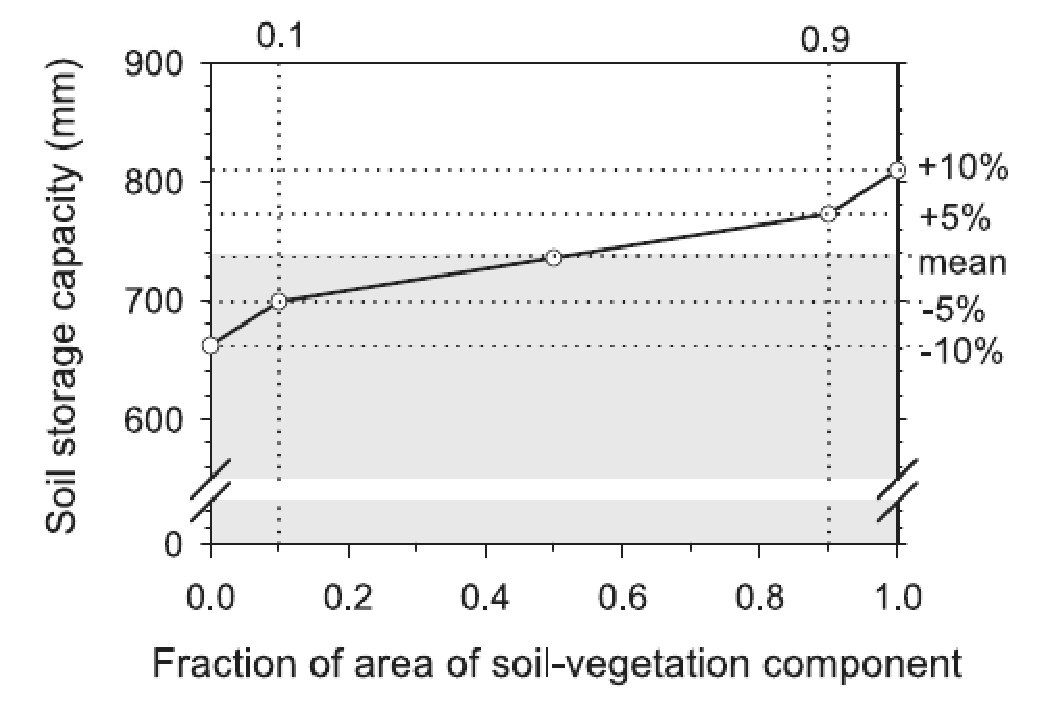
\includegraphics[width=\columnwidth]{\figdir/f_saturation.eps}
  \caption[Example of saturated fraction of a soil unit.]{Example for the computation of saturated fraction of a soil unit from actual water content as given by \eqnref{eq:f_sat}. Graphic copied from \citet{Guentner2002}. \textbf{Units shown deviate from \eqnref{eq:f_sat}!} \label{fig:f_sat}}
\end{figure}

When using function \verb!f_saturation! saturation excess flow can be determined by multiplying incoming surface water flux with the saturated areal fraction of the soil. The remaining part can be given to the infiltration routine. If \verb!f_saturation! is not used saturation excess surface runoff occurs only when the soil is completely saturated (you should check that before calling \verb!infiltration! in order to be able to deviate the two types of surface runoff).


\subsubsection{Subsurface runoff}
Subsurface runoff within the physical based approach can be directly determined from lateral excess runoff (i.e. simply the output of function \verb!latflow!). Further discrimination between a faster (e.g. preferential flow) and slower component is so far not possible.


\subsubsection{Groundwater runoff}
Groundwater runoff (or \emph{baseflow} although in some definitions this also includes slow subsurface runoff) can be deviated from function \verb!percolation!. It is simply the percolation from the deepest soil horizon. To account for travel time through an unsaturated zone below the soil profile a storage routing approach could be applied before adding the percolation output to the groundwater storage.



%%%%%%%%%%%%%%%%%%%%%%%%%%%%%%%%%%%%%%%%%%%%%%%%%%%%%%%%%%%%%%%%%%%%%%%%%%%%%%%%
%%%%%%%%%%%%%%%%%%%%%%%%%%%%%%%%%%%%%%%%%%%%%%%%%%%%%%%%%%%%%%%%%%%%%%%%%%%%%%%%
%%%%%%%%%%%%%%%%%%%%%%%%%%%%%%%%%%%%%%%%%%%%%%%%%%%%%%%%%%%%%%%%%%%%%%%%%%%%%%%%
%%%%%%%%%%%%%%%%%%%%%%%%%%%%%%%%%%%%%%%%%%%%%%%%%%%%%%%%%%%%%%%%%%%%%%%%%%%%%%%%
%%%%%%%%%%%%%%%%%%%%%%%%%%%%%%%%%%%%%%%%%%%%%%%%%%%%%%%%%%%%%%%%%%%%%%%%%%%%%%%%




\section{Contributions and TODOs}
The following work still has to be done or issues need to be resolved:

\begin{itemize}
\item Add more approaches, e.g.
  \begin{itemize}
    \item Better approximation of sorptivity and suction at wetting front \citep{Stewart2013}
    \item Horton: account for soil moisture state and discrete time steps/intermittent rainfall (promising approaches: \citet{Ludwig2010en,Bauer1974,Green1986,Rossman2016})
  \end{itemize}
\item Create separate function to calculate unsaturated hydraulic conductivity and matric potential with several alternatives (so far only \emph{Van Genuchten} considered; could be extended by, e.g., \emph{Brooks and Corey} and/or \emph{Campbell}, \citet{Maidment1993})
\item Include macro pore/preferential flow
\item Include capillary rise
\item Account for ponding of soil profile from lower layers
\item Somehow possible to include the Richards equation? Must be solved numerically, I think each soil layer would have to be somehow subdivided into smaller instances during solving...
\end{itemize}

\include{chapters/part_processes/runoffConcentration/runoffConcentration}
\include{chapters/part_processes/channelFlow/channelFlow}
\include{chapters/part_processes/evaporation/evaporation}
\chapter{Evapotranspiration} \label{chap:et}
\renewcommand{\tabdir}{chapters/part_processes/evapotranspiration/tab}
\renewcommand{\figdir}{chapters/part_processes/evapotranspiration/fig}

\section{Introduction} \label{sec:et:intro}

This chapter describes approaches to model evapotranspiration. Two distinct calculation procedures exist:
\begin{enumerate}
  \item Computation of a \emph{potential} evapotranspiration rate \etPot. This represents the maximum possible rate in the absence of water stress. It is basically limited by energy supply.
  \item Estimation of the \emph{actual} evapotranspiration rate \etReal{} taking into account the properties of vegetation and the limitation by a soil moisture deficit.
\end{enumerate}

Over past decades a large number of approaches has been developed, ranging from simple empirical to complex process-based ones. For a review of the historical development of both scientific knowledge and modeling of evapotranspiration the reader is referred to \cite{Shuttleworth2007}.

Each of the functions introduced in the next sections can be called independently. However, to have a greater flexibility 'master functions' where defined taking all possible input variables and parameters, and a choice flag (in a model application this would preferably be a \verb!sharedParamNum!) internally calling the desired method with all relevant inputs. Note that, in general, all inputs have to be given but can be set to a dummy value in case it is not needed for the desired method. The master function \verb!et_pot! calculates \emph{potential} evapotranspiration whereas \verb!et_act! calculates the \emph{actual} value. The output unit is, as commonly done in ECHSE, defined following the international SI system: [\si{\metre\per\second}]. This can be adapted in the implementation of you model engine. E.g., to derive a \emph{sum} of evapotranspiration instead of an average \emph{flux} over the simulation time step multiply by \verb!delta_t! (in [\si{\second}]) and by \num{1000} to get [\si{\milli\metre}]. \tabsref{tab:et:pot} and \ref{tab:et:act} list all input variables for the master functions in the order of occurrence (however, you are advised to look into the source code in case changes have not yet been included into the documentation!).

If the functions are called with hourly time steps it may happen that negative evapotranspiration is calculated due to a negative energy balance (outgoing energy predominates incoming energy). This can be interpreted as dew formation. However, so far this process is not explicitly considered and the result of every evapotranspiration routine is limited to zero as lower boundary.

In the following the procedures so far incorporated in ECHSE shall be briefly described. Note that many approaches make use of meteorological quantities and relationships which are independently described in \chapref{chap:meteo}.

\onecolumn
\begin{center}
\tablecaption{Argument list for ECHSE's master function \emph{et\_pot} in the order of occurrence (check the source code for the case of unreported changes!).  \label{tab:et:pot}}
\tablefirsthead{}
\tablehead{
\multicolumn{5}{l}{\emph{Continued from previous page.}}\\ \hline
}
\tabletail{
\hline
\multicolumn{5}{l}{\emph{Continued on next page.}}\\
}
\tablelasttail{}
\begin{supertabular}{|p{0.06\textwidth}p{0.15\textwidth}p{0.05\textwidth}p{0.23\textwidth}p{0.36\textwidth}|} \hline
\rowcolor[gray]{0.9}
\hline
Symbol & Identifier & Unit & Explanation & Comment \\ \hline
\multicolumn{5}{|l|}{Common meteorological variables}\\ \hline
\airtemp & \verb!temper! & \si{\degreeCelsius} & Mean air temperature over time step & Mandatory; estimated from \airtempMin{} and \airtempMax{} if it is missing \\
\airtempMin & \verb!temp_min! & \si{\degreeCelsius} & Minimum air temperature within time step & Currently only used to estimate \airtemp{} if it is missing \\
\airtempMax & \verb!temp_max! & \si{\degreeCelsius} & Maximum air temperature within time step & Currently only used to estimate \airtemp{} if it is missing \\
\radShortwaveIn & \verb!glorad! & \si{\watt\per\metre\squared} & Incoming short-wave radiation & Needed for energy balance based approaches; commonly measured but can be estimated from \verb!radex!, \verb!sundur!, \verb!cloud!, \verb!lat!, \verb!doy!, \verb!radex_a!, and \verb!radex_b!, \secref{sec:meteo:radshort} \\
\relHumidity & \verb!rhum! & \si{\percent} & Relative humidity of air & Calculation of vapor pressure \\
\windspeed & \verb!wind! & \si{\metre\per\second} & Wind speed averaged over time step & Estimation of \emph{aerodynamic resistance}, see \secref{sec:et:resist} \\
\airPressure & \verb!apress! & \si{\hecto\pascal} & Air pressure at location & Estimation of \psychroConst{} and \densityAir{}; can also be estimated from \verb!elev!, \secref{sec:meteo:apress} \\
\sundur & \verb!sundur! & \si{\hour} & Measured sunshine duration over time step & Calculation of \radShortwaveIn{} in case it is missing \\
\cloudFraction & \verb!cloud! & \si{\percent} & Percentage of cloudiness & Not yet fully incorporated but included in the interface (use a dummy value)! \\
\hline
\multicolumn{5}{|l|}{Common site-secific parameters}\\ \hline
\lat & \verb!lat! & dec. \si{\degree} & Latitude & Needed for calculation of \radExtraterr{} and \radShortwaveIn{}; use positive values for northern and negative values for southern hemisphere \\
\lon & \verb!lon! & dec. \si{\degree} & Longitude & Currently only needed to calculate \radExtraterr{} at hourly resolution; defined as degrees west of Greenwich meridian, e.g. Greenwich: \SI{0}{\degree}, New York: \SI{75}{\degree}, Berlin: \SI{346.5}{\degree} \\
$h$ & \verb!elev! & \si{\metre} & Elevation above sea level & Needed for calculation of \airPressure{} and \radShortwaveInClearsky{}\\
\hline
\multicolumn{5}{|l|}{Quantities of energy balance (commonly calculated internally)}\\ \hline
\radExtraterr & \verb!radex! & \si{\watt\per\metre\squared} & Extraterrestrial radiation & Needed for energy balance based approaches; usually calculated from \verb!lat! and \verb!doy! (daily resolution) or \verb!lat!, \verb!doy!, \verb!hour!, \verb!utc_add!, and \verb!L_m! (hourly resolution), \secref{sec:meteo:radex} \\
\radShortwaveInClearsky & \verb!glorad_max! & \si{\watt\per\metre\squared} & Incoming short-wave radiation under clear sky & Needed for energy balance based approaches to calculate the cloudiness correction factor; usually calculated from \verb!radex! and \verb!radex_a!, \verb!radex_b! or \verb!elev! \secref{sec:meteo:radshortmax} \\
\netRadiation & \verb!H_net! & \si{\watt\per\metre\squared} & Net incoming short-wave + long-wave radiation & Needed for energy balance based approaches; usually calculated from a range of meteorological variables and parameters, see \secref{sec:meteo:radnet} \\
\netRadiationSoil & \verb!H_soil! & \si{\watt\per\metre\squared} & Net incoming short-wave + long-wave radiation directly at soil surface & Needed for energy balance in SW approach (\secref{sec:et:sw}) \\
\netRadiationLong & \verb!H_long! & \si{\watt\per\metre\squared} & Net incoming long-wave radiation & Needed for energy balance based approaches; usually calculated from a range of meteorological variables and parameters, see \secref{sec:meteo:radnetlong} \\
\heatfluxSoil & \verb!soilheat! & \si{\watt\per\metre\squared} & Soil heat flux & Needed for energy balance based approaches; usually calculated, see \secref{sec:meteo:soilflux}; in SW calculated from \netRadiationSoil{} instead of \netRadiation{} \\
\heatfluxVegSoil & \verb!totalheat! & \si{\watt\per\metre\squared} & Heat flux into soil AND storage of physical and biochemical energy in vegetation and atmosphere below measurement height & Needed for energy balance in SW approach (\secref{sec:et:sw}); so far calculated just as \heatfluxSoil{} from \netRadiation{} \\
\hline
\multicolumn{5}{|l|}{Meteorological parameters}\\ \hline
\measHeightTemp & \verb!h_tempMeas! & \si{\metre} & Measurement height of air temperature & Calculation of \emph{aerodynamic resistance}, see \secref{sec:et:resist}; usually \SI{2}{\metre}\\
\measHeightRelhum & \verb!h_humMeas! & \si{\metre} & Measurement height of relative humidity & Calculation of \emph{aerodynamic resistance}, see \secref{sec:et:resist}; usually \SI{2}{\metre}\\
\measHeightWind & \verb!h_windMeas! & \si{\metre} & Measurement height of wind speed & Calculation of \emph{aerodynamic resistance}, see \secref{sec:et:resist}; usually \SI{2}{\metre}\\
\emisa{},\emisb{} & \verb!emis_a!, \verb!emis_b! & -- & Emissivity parameters & See \secref{sec:meteo:emiss}\\
\cloudCorrFacA{},\cloudCorrFacB{} & \verb!fcorr_a!, \verb!fcorr_b! & -- & Cloudiness coefficients & Parameters for calculation of \cloudCorrFac{}, see \secref{sec:meteo:cloudcorr}\\
\angstA{},\angstB{} & \verb!radex_a!, \verb!radex_b! & -- & {\AA}ngström coefficients & Calculation of \radShortwaveIn{} and \radShortwaveInClearsky{}, see \secsref{sec:meteo:radshort}, \ref{sec:meteo:radshortmax}\\
\soilheatDay{},\soilheatNight{} & \verb!f_day!, \verb!f_night! & -- & Coefficients for soil heat flux calculation & Calculation of \heatfluxSoil{}, see \secref{sec:meteo:soilflux}\\
\hline
\multicolumn{5}{|l|}{Vegetation and land-cover parameters and variables}\\ \hline
\cropfacMak & \verb!crop_makk! & -- & Crop factor \emph{Makkink} & Calculation of land-cover specific \etPot{} after \emph{Makkink}, cf. \secref{sec:eta:cropfactors} \\
\cropfacFAO & \verb!crop_faoref! & -- & Crop factor \emph{FAO reference} & Calculation of land-cover specific \etPot{} following \emph{FAO reference evaporation model}, cf. \secsref{sec:et:fao_ref}, \ref{sec:eta:cropfactors}; simply set it to one if you want the reference evaporation \\
\canoHeight & \verb!cano_height! & \si{\metre} & Canopy height & Calculation of \emph{aerodynamic resistance}, cf. \secref{sec:et:resist} \\
\leafAreaIndex & \verb!lai! & \si{\metre\squared\per\metre\squared} & Leaf area index & Calculation of \emph{resistances}, cf. \secref{sec:et:resist} \\
\albedo & \verb!alb! & -- & Albedo & Calculation of energy balance (\netRadiation{}), see \secref{sec:meteo:radnet} \\
\canoExt & \verb!ext! & -- & Canopy's extinction coefficient & Extinction of incoming radiation by canopy expressed by the \emph{Beer-Lambert law}; needed for calculation of canopy surface resistance, see \secref{sec:et:resist} \\
\resLeafMin & \verb!res_leaf_min! & \si{\second\per\metre} & Minimum stomatal resistance of a single leaf & Species-specific parameter; value gets up-scaled to whole canopy for calculation of canopy surface resistance, see \secref{sec:et:resist} \\
\densitySoil & \verb!soil_dens! & \si{\kilo\gram\per\cubic\metre} & Bulk density of soil & Calculation of soil's \emph{surface resistance}; only for approaches explicitly accounting for surface resistance of soil, see \secref{sec:et:res:rss} \\
\radShortHalf & \verb!glo_half! & \si{\watt\per\metre\squared} & Short-wave radiation at which stomatal conductance is half of its maximum & Species-specific parameter for calculation of canopy resistance, see \eqnref{eqn:et:res:rcs2} \\
\resMeanBound & \verb!res_b! & \si{\second\per\metre} & Mean boundary layer resistance & Parameter bulk boundary layer aerodynamic resistance of vegetative elements in the canopy; for two-layer approaches, see \secref{sec:et:res:rca} \\
\dragCoef & \verb!drag_coef! & -- & Effective value of mean drag coefficient of vegetative elements & Parameter for calculation of aerodynamic resistance using approach of \citet{Shuttleworth1990}, see \secref{sec:et:resist} \\
\roughSoil & \verb!rough_bare! & \si{\metre} & Roughness length of bare soil & Parameter for calculation of aerodynamic resistance, see \secref{sec:et:resist} \\
\eddyDecay & \verb!eddy_decay! & -- & Eddy diffusivity decay constant & Parameter for calculation of aerodynamic resistance using approach of \citet{Shuttleworth1985}, see \secref{sec:et:resist} \\
\rssa{}, \rssb{} & \verb!rss_a!, \verb!rssb! & -- & Parameters for calculation of soil surface resistance & Empirical parameters for calculation of soil surface resistance (needed for two-layer approaches) following \citet{Domingo1999}, see \secref{sec:et:resist} \\
\hline
\multicolumn{5}{|l|}{Computational parameters}\\ \hline
\doy & \verb!doy! & -- & Day of the year (Julian day) & Calculation of \radShortwaveIn{} and \radExtraterr{} \\
\hour & \verb!hour! & -- & Hour of day & Value in the range of \{0..23\}; only needed for calculation of hourly values of \radExtraterr{} \\
\utcAdd & \verb!utc_add! & \si{\hour} & Deviation of local time zone from UTC & Value in the range of \{\num{-12}..\num{14}\}; can vary over the year due to daylight saving time; only needed for calculation of hourly values of \radExtraterr{} \\
-- & \verb!na_val! & -- & Numeric value treated as \emph{not available (NA)} & Input quantities having the specified value will be internally treated as NA (e.g. for input checks) \\
\deltat & \verb!delta_t! & \si{\second} & Time step length & Temporal resolution of the model; \textbf{use ECHSE's internal parameter!} (only argument for the \verb!simulate! method, cf. \citet{Echse-Main-Doc}) \\
\hline
\multicolumn{5}{|l|}{Choice flags}\\ \hline
-- & \verb!choice! & -- & Choice of potential evapotranspiration model & 1: Makkink \newline 11: Penman-Monteith \newline 12: FAO reference evaporation \\
-- & \verb!ch_rcs! & -- & Choice of canopy stomatal resistance model & See \secref{sec:et:resist} \\
-- & \verb!ch_roughLen! & -- & Choice for calculation of roughness length & For calculation of aerodynamic resistance, \secref{sec:et:resist} \\
-- & \verb!ch_plantDispl! & -- & Choice for calculation of displacement height & For calculation of aerodynamic resistance, \secref{sec:et:resist} \\
-- & \verb!ch_gloradmax! & -- & Choice for calculation of \radShortwaveInClearsky{} & See \secref{sec:meteo:radshortmax} \\
\hline
\end{supertabular}
\end{center}


\begin{center}
\tablecaption{Arguments for ECHSE's master function \emph{et\_act} \textbf{in addition} to those for \emph{et\_pot} listed in \tabref{tab:et:pot} (check the source code for the case of unreported changes!).  \label{tab:et:act}}
\tablefirsthead{}
\tablehead{
\multicolumn{5}{l}{\emph{Continued from previous page.}}\\ \hline
}
\tabletail{
\hline
\multicolumn{5}{l}{\emph{Continued on next page.}}\\
}
\tablelasttail{}
\begin{supertabular}{|p{0.06\textwidth}p{0.15\textwidth}p{0.05\textwidth}p{0.23\textwidth}p{0.36\textwidth}|} \hline
\rowcolor[gray]{0.9}
\hline
Symbol & Identifier & Unit & Explanation & Comment \\ \hline
\waterContTop & \verb!wc_vol_top! & \si{\cubic\metre\per\cubic\metre} & Volumetric water content of the top-most soil horizon & Needed for estimation of resistance against soil evaporation (\secref{sec:et:res:rss}) \\
\waterContRoot & \verb!wc_vol_root! & \si{\cubic\metre\per\cubic\metre} & Volumetric water content of the root zone & Needed for estimation of soil moisture factor (\secref{sec:eta:soilmoisture}) or resistance against plant transpiration (\secref{sec:et:res:rcs}) \\
\waterContSat & \verb!wc_sat! & \si{\cubic\metre\per\cubic\metre} & Volumetric water content at saturation of the root zone & Needed for estimation of resistance against plant transpiration (\secref{sec:et:res:rcs}) \\
\waterContPwp & \verb!wc_pwp! & \si{\cubic\metre\per\cubic\metre} & Volumetric water content of the root zone at permanent wilting point & Needed for estimation of soil moisture factor (\secref{sec:eta:soilmoisture}) \\
\waterContRes & \verb!wc_res! & \si{\cubic\metre\per\cubic\metre} & Residual volumetric water content of the root zone & Needed for estimation of resistance against plant transpiration (\secref{sec:et:res:rcs}) \\
\waterContEtmax & \verb!wc_etmax! & \si{\cubic\metre\per\cubic\metre} & Parameter giving the minimum volumetric water content for actual evapotranspiration to be equal to the potential one & Needed for estimation of soil moisture factor (\secref{sec:eta:soilmoisture}); typically $\frac{\waterContEtmax}{\waterContFK}$ is a value of [\num{0.5}..\num{0.8}] with \waterContFK{} being \emph{field capacity} \\
\bubblePress & \verb!bubble! & \si{\hecto\pascal} & Bubbling pressure of the root zone & Needed for estimation of resistance against plant transpiration (\secref{sec:et:res:rcs}); Parameter can be derived by pedotransfer functions; note that unit [\si{\hecto\pascal}] is approximately equal to [\si{\centi\metre} of water] \\
\PoresInd & \verb!pores_ind! & -- & Pore-size-index of the root zone & Needed for estimation of resistance against plant transpiration (\secref{sec:et:res:rcs}); Parameter can be derived by pedotransfer functions \\
\sucStressMin & \verb!wstressmin! & \si{\hecto\pascal} & Capillary suction at minimum water stress (stomata completely open) & Needed for estimation of resistance against plant transpiration (\secref{sec:et:res:rcs}); Species-specific plant parameter; note that unit [\si{\hecto\pascal}] is approximately equal to [\si{\centi\metre} of water] \\
\sucStressMax & \verb!wstressmax! & \si{\hecto\pascal} & Capillary suction at maximum water stress (total stomata closure, wilting point) & Needed for estimation of resistance against plant transpiration (\secref{sec:et:res:rcs}); Species-specific plant parameter; note that unit [\si{\hecto\pascal}] is approximately equal to [\si{\centi\metre} of water] \\
\condVapPressPar & \verb!par_stressHum! & \si{\per\hecto\pascal} & Empirical parameter & Needed for calculation of water vapor deficit stomatal conductance stress factor (\secref{sec:et:res:rcs}) \\
\hline
\end{supertabular}
\end{center}
\twocolumn


%%%%%%%%%%%%%%%%%%%%%%%%%%%%%%%%%%%%%%%%%%%%%%%%%%%%%%%%%%%%%%%%%%%%%%%%%%%%%%%%
%%%%%%%%%%%%%%%%%%%%%%%%%%%%%%%%%%%%%%%%%%%%%%%%%%%%%%%%%%%%%%%%%%%%%%%%%%%%%%%%
%%%%%%%%%%%%%%%%%%%%%%%%%%%%%%%%%%%%%%%%%%%%%%%%%%%%%%%%%%%%%%%%%%%%%%%%%%%%%%%%
%%%%%%%%%%%%%%%%%%%%%%%%%%%%%%%%%%%%%%%%%%%%%%%%%%%%%%%%%%%%%%%%%%%%%%%%%%%%%%%%
%%%%%%%%%%%%%%%%%%%%%%%%%%%%%%%%%%%%%%%%%%%%%%%%%%%%%%%%%%%%%%%%%%%%%%%%%%%%%%%%


\section{Models} \label{sec:et:models}

\subsection{Empirical equations}\label{sec:et:emp}


% ATTENTION: commented out Hargreaves model as I think there is an error:
% incoming short-wave radiation should actually be extraterrestrial radiation?!
% It is furthermore not included in ECHSE
%\subsection{Hargreaves model} \label{sec:et:pot:hargreaves}
%
%This is a very simply model yielding estimates of \etPot{} with daily resolution. It requires as input
%\begin{itemize}
%  \item Incoming short-wave radiation
%  \item Daily minimum and maximum temperature
%\end{itemize}
%
%If the radiation is given as a daily average value (instead of a sum), the Hargreaves model takes the form of \eqnref{eqn:et:pot:hargreaves}
%
%\begin{align} \label{eqn:et:pot:hargreaves}
%  \etPot = & CH \cdot \left( \frac{t_{max}+t_{min}}{2} + CT \right) \cdot \\
%           & \sqrt{t_{max}-t_{min}} \cdot 0.0864 \cdot \radShortwaveIn{} \nonumber
%\end{align}
%
%with
%
%\medskip
%\begin{tabular}{p{0.25\columnwidth}p{0.55\columnwidth}}
%  \etPot & Hargreaves potential evapotranspiration rate (mm/day) \\
%  $t_{max}$, $t_{min}$ & Daily minimum and maximum of air temperature (\celsius) \\
%  \radShortwaveIn{} & Daily average of incoming short-wave radiation (W/\sqm{}) \\
%  0.0864 & Factor to convert \radShortwaveIn{} from W/\sqm{} into MJ/\sqm{}/day \\
%  $CH$ & Empirical coefficient, $CH$= 0.0023 \\
%  $CT$ & Empirical coefficient, $CT$= 17.8 \\
%\end{tabular}


\subsubsection{Makkink model} \label{sec:et:makkink}

The Makkink model is simple approach to estimate potential evaporation using only temperature (\verb!temper!), downward short-wave radiation (\verb!glorad!), and air pressure (\verb!apress!; or estimated from elevation, see \secref{sec:meteo:apress}) as predictors. The approach is discussed in detail by \citet{deBruin1987, Feddes1987, Hiemstra2011}.

Using convenient units, the basic equation without an additive empirical constant \citep[see][]{deBruin1987} is \eqnref{eqn:et:makkink}

\begin{equation} \label{eqn:et:makkink}
  \etPot = c \cdot \frac{s}{s + \gamma} \cdot \frac{\radShortwaveIn}{1000 \cdot \evapHeatWater \cdot \densityWater}
\end{equation}

\noindent
usage
\begin{verbatim}
et_pot_makkink(glorad,temper,apress,
cropfactor)
\end{verbatim}

\noindent
with\\ \vspace*{2ex}

\noindent
\medskip
\begin{tabular}{lp{0.8\columnwidth}}
  \etPot & Makkink reference crop-evaporation (m/s) \\
  $s$ & Slope of the curve of saturation water vapor pressure (kPa / K); see \secref{sec:meteo:slopevappress} \\
  $\gamma$ & Psychrometric constant (kPa / K); see \secref{sec:meteo:psychro} \\
  $\radShortwaveIn$ & Incoming short-wave radiation (W/\sqm{}); see \secref{sec:meteo:radshort} \\
  $\evapHeatWater$ & Latent heat of water evaporation (kJ/kg); see \secref{sec:meteo:evapheat} \\
  $\densityWater$ & Density of water ($\approx$ 1000 kg/\cbm{}) \\
  $1000$ & Factor to convert kJ into J \\
  $c$ & Dimensionless empirical constant, $c$=0.65 \\
\end{tabular}\\

\textbf{Note} that, to derive \etPot{} for a specific site with certain land-cover, \eqnref{eqn:et:makkink} still has to be multiplied by a crop factor (\verb!cropfactor!, see \secref{sec:eta:cropfactors}). Accounting for soil moisture deficit will finally lead to \emph{actual} evapotranspiration \etReal{} (see \secref{sec:eta:soilmoisture}).



%%%%%%%%%%%%%%%%%%%%%%%%%%%%%%%%%%%%%%%%%%%%%%%%%%%%%%%%%%%%%%%%%%%%%%%%%%%%%%%%
%%%%%%%%%%%%%%%%%%%%%%%%%%%%%%%%%%%%%%%%%%%%%%%%%%%%%%%%%%%%%%%%%%%%%%%%%%%%%%%%

\subsection{Process-based approaches}\label{sec:et:proc}

\subsubsection{Penman-Monteith equation} \label{sec:et:penmon}

The famous equation of \emph{Penman-Monteith} is a widely used physically-based approach of modelling evapotranspiration. That means, in contrast to purely empirical approaches, it explicitly simulates the governing physical processes whereas the individual components, however, might still rely on empirical relationships. 

The formula takes into account the energy available for evapotranspiration in the canopy and the vapor pressure deficit. It further incorporates resistance to evapotranspiration due to \emph{(a)} stomatal resistance of the canopy, i.e. the movement of water through the stomata of leaves controlled by the plant, termed \emph{surface resistance}, and \emph{(b)} the transfer of water vapor from the surface of evapotranspiration into the atmosphere by turbulent diffusion, termed \emph{aerodynamic resistance}, which is controlled by wind speed and the roughness of the surface. In analogy to \emph{Ohm's law} applied in electrotechnic the resistances are treated as a network of resistances connected in series.

The \emph{Penman-Monteith} equation further relies on the \emph{big leaf} simplification, i.e. the vegetation canopy is treated as a single big leaf, and the vegetation being uniformly distributed over the area of interest neglecting evaporation from bare soil. The relation should therefore be applied only at sites of uniform crop vegetation with closed canopy. Over forests and sites of heterogeneous and/or sparse (natural) vegetation with exposed soil the \emph{big leaf} approach would be inoperative.

More detailed information on the model can be obtained from textbooks, e.g. \citet{Maidment1993} or \citet{Dyck1995}. The formula is:

\begin{multline} \label{eqn:et:penmon}
  \etPot =  \frac{1}{\evapHeatWater{}} \\
  \left[ \frac{\slopeSatVapCurve{} (\netRadiation{} - \heatfluxSoil{}) + \densityAirMoist{} \specHeatAir{} (\satVaporPressure{} - \vaporPressure{}) / \resAero}{\slopeSatVapCurve{} + \psychroConst{} (1 + \resCanopy / \resAero)} \right]
\end{multline}

\noindent
usage
\begin{verbatim}
etp_penmon(lambda,delta,H_net,G,
rho_air,ez_0,ez,gamma,r_c,r_a)
\end{verbatim}

\noindent
with\\ \vspace*{2ex}

\tablefirsthead{}
\tablehead{}
\tabletail{}
\tablelasttail{}
\begin{supertabular}{lp{0.8\columnwidth}}
  \etPot & Potential evapotranspiration under given meteorological and land-cover conditions assuming unlimited water supply (m/s) \\
  \evapHeatWater & Latent heat of water evaporation; see \secref{sec:meteo:evapheat} \\
  \slopeSatVapCurve & Slope of the curve of saturation water vapor pressure; see \secref{sec:meteo:slopevappress} \\
  \netRadiation & Incoming net (short- and long-wave) radiation; see \secref{sec:meteo:radnet} \\
  \heatfluxSoil & Soil heat flux; see \secref{sec:meteo:soilflux} \\
  \densityAirMoist & Density of air; see \secref{sec:meteo:densairmoist} \\
  \specHeatAir & Specific heat of moist air; see \secref{sec:meteo:constants} \\
  \satVaporPressure & Water vapor pressure at saturation; see \secref{sec:meteo:satvappress} \\
  \vaporPressure & Water vapor pressure; see \secref{sec:meteo:vappress} \\
  \psychroConst & Psychrometric constant; see \secref{sec:meteo:psychro} \\
  \resAero & Aerodynamic resistance; see \secref{sec:et:resist} \\
  \resCanopy & Canopy surface resistance; see \secref{sec:et:resist} \\
\end{supertabular}\\


\subsubsection{FAO reference evaporation} \label{sec:et:fao_ref}
The \emph{Food and Agricultural Organization of the United Nations (FAO)} published guidelines for the computation of crop water requirements by estimation of evapotranspiration based on the \emph{Penman-Monteith} equation which are freely accessible online via \url{http://www.fao.org/docrep/X0490E/x0490e00.htm}. For simplification and generalization a so-called \emph{reference crop} was defined, a hypothetical well-watered and uniform grass vegetation of \SI{0.12}{\metre} height with a fixed \emph{surface resistance} of \SI{70}{\second\per\metre} and an albedo of \num{0.23}. For the calculation of potential evapotranspiration for that reference vegetation (\etRef{} in \si{\metre\per\second}), the so-called \emph{FAO reference evaporation}, two approaches for daily and hourly time steps, respectively, have been adopted and implemented into ECHSE:

\begin{multline} \label{eqn:et:fao_ref_d}
  \etRefDaily = \\
  \frac{0.408 \slopeSatVapCurve{} (\netRadiation{} - \heatfluxSoil{}) + \psychroConst \frac{900}{\airtemp + 273} \windspeed (\satVaporPressure{} - \vaporPressure{})}{\slopeSatVapCurve{} + \psychroConst{} (1 + 0.34 \windspeed)}
\end{multline}
\begin{multline} \label{eqn:et:fao_ref_h}
  \etRefHourly = \\
  \frac{0.408 \slopeSatVapCurve{} (\netRadiation{} - \heatfluxSoil{}) + \psychroConst \frac{37}{\airtemp + 273} \windspeed (\satVaporPressure{} - \vaporPressure{})}{\slopeSatVapCurve{} + \psychroConst{} (1 + 0.34 \windspeed)}
\end{multline}


\noindent
usage
\begin{verbatim}
etp_penmon_ref(temper,wind,
apress,delta,H_net,G,ez_0,ez,
h_windMeas,delta_t)
\end{verbatim}

\noindent
with\\ \vspace*{2ex}

\tablefirsthead{}
\tablehead{}
\tabletail{}
\tablelasttail{}
\begin{supertabular}{lp{0.8\columnwidth}}
  \etRef & FAO reference evaporation (\si{\metre\per\second}) \\
  \airtemp & Air temperature (\si{\degreeCelsius}) \\
  \windspeed & Wind speed (\si{\metre\per\second}) \\
  \slopeSatVapCurve & Slope of the curve of saturation water vapor pressure; see \secref{sec:meteo:slopevappress} \\
  \netRadiation & Incoming net (short- and long-wave) radiation; see \secref{sec:meteo:radnet} \\
  \heatfluxSoil & Soil heat flux; see \secref{sec:meteo:soilflux} \\
  \satVaporPressure & Water vapor pressure at saturation; see \secref{sec:meteo:satvappress} \\
  \vaporPressure & Water vapor pressure; see \secref{sec:meteo:vappress} \\
  \psychroConst & Psychrometric constant; see \secref{sec:meteo:psychro} \\
\end{supertabular}\\ \vspace*{2ex}


This simplified approach can be used if necessary data to apply \eqnref{eqn:et:penmon} are not available. However, to actually derive the potential evapotranspiration for your location you still need to multiply the result with a land-cover specific \emph{crop factor} (cf. \secref{sec:eta:cropfactors}).

\textbf{Note} that applying this simplified relation may result in some errors due to the amount of implicit assumptions. Especially when hourly values are calculated the presumed constant value of \emph{surface resistance} over the whole day may lead to underprediction over daytime and overpredictions over nighttime where errors should compensate one another when summed over the day.

\textbf{Note} that internal adjustments are applied which are not shown in the presented equations to derive the mentioned units from the reported units of input variables.


\subsubsection{Shuttleworth-Wallace} \label{sec:et:sw}
The model of \citet{Shuttleworth1985} (henceforth also termed \textbf{SW model}) is an enhancement of the \emph{Penman-Monteith} equation (\secref{sec:et:penmon}). It relaxes the \emph{big leaf} assumption by an advanced resistance scheme to better account for a clumped vegetation containing patches of bare soil. The model is thus suitable for application in semi-arid environments and over agricultural fields containing sparse crops without a closed canopy. Yet it should be not applied at forest sites.

The approach uses a one-dimensional model of energy partition into a part for closed vegetation and bare soil, respectively. It further introduces additional resistances to account for the resistance of soil against evaporation. Transpiration from the canopy \etTransp{} (in [\si{\metre\per\second}]) and evaporation from bare soil \etEvap{} (in [\si{\metre\per\second}]) can then be separately calculated as:

\begin{multline} \label{eqn:et:sw_ets}
\etEvap =  \frac{1}{\evapHeatWater} \left[ \frac{\slopeSatVapCurve A_s + \densityAirMoist \specHeatAir \vapPresDefCano / \resSA}{\slopeSatVapCurve + \psychroConst (1 + \resSoil / \resSA)} \right]
\end{multline}

\noindent
usage
\begin{verbatim}
et_sw_soil(lambda,delta,H_soil,
soilheat,rho_air,D_0,gamma,
r_ss,r_sa)
\end{verbatim}

\begin{multline} \label{eqn:et:sw_etc}
\etTransp =  \frac{1}{\evapHeatWater} \left[ \frac{\slopeSatVapCurve (A - A_s) + \densityAirMoist \specHeatAir \vapPresDefCano / \resCA}{\slopeSatVapCurve + \psychroConst (1 + \resCanopy / \resCA)} \right]
\end{multline}

\noindent
usage
\begin{verbatim}
et_sw_cano(lambda,delta,H_net,
H_soil,totalheat,soilheat,
rho_air,D_0,gamma,r_cs,r_ca)
\end{verbatim}

\noindent
with\\ \vspace*{2ex}

\tablefirsthead{}
\tablehead{}
\tabletail{}
\tablelasttail{}
\begin{supertabular}{lp{0.75\columnwidth}}
  \evapHeatWater & Latent heat of water evaporation; see \secref{sec:meteo:evapheat} \\
  \slopeSatVapCurve & Slope of the curve of saturation water vapor pressure; see \secref{sec:meteo:slopevappress} \\
  $A_s$ & Total energy available at soil surface: $A_s = \netRadiationSoil - \heatfluxSoil$ \\
  $A$ & Total energy available at measurement height (above canopy): $A = \netRadiation - \heatfluxVegSoil$ \\
  \netRadiation & Incoming net (short- and long-wave) radiation; see \secref{sec:meteo:radnet} \\
  \netRadiationSoil & Incoming net (short- and long-wave) radiation hitting the soil surface \\
  \heatfluxSoil & Soil heat flux; see \secref{sec:meteo:soilflux} \\
  \heatfluxVegSoil & Heat flux into soil AND vegetation \\
  \densityAirMoist & Density of air; see \secref{sec:meteo:densairmoist} \\
  \specHeatAir & Specific heat of moist air; see \secref{sec:meteo:constants} \\
  \vapPresDefCano & Vapor pressure deficit \textbf{at canopy source height} \\
  \psychroConst & Psychrometric constant; see \secref{sec:meteo:psychro} \\
  \resCA & Bulk boundary layer resistance of the vegetative elements in the canopy; see \secref{sec:et:resist} \\
  \resCanopy & Canopy surface resistance; see \secref{sec:et:resist} \\
  \resSA & Aerodynamic resistance between soil and canopy source height; see \secref{sec:et:resist} \\
  \resSoil & Surface resistance of soil; see \secref{sec:et:resist} \\
\end{supertabular}\\ \vspace*{2ex}

To calculate the vapor pressure deficit at canopy source height \vapPresDefCano{} either measurements of air temperature and relative humidity at canopy source height have to be given (\vapPresDefCano{} can then be calculated as described in \secref{sec:meteo:vappressdef}) or from the energy balance whereas the total latent heat flux ($\evapHeatWater \et$) has already to be known:

\begin{multline} \label{eqn:et:sw_d0}
\vapPresDefCano =  \vaporPressureDeficit + \frac{\resAero}{\densityAirMoist \specHeatAir} \left[ \slopeSatVapCurve A - (\slopeSatVapCurve + \psychroConst) \evapHeatWater \et \right]
\end{multline}

\noindent
usage
\begin{verbatim}
vapPressDeficit_canopy(H_net,
totalheat,gamma,delta,lambda,
vapPressDeficit,r_aa,et_total,
rho_air)
\end{verbatim}

\noindent
with\\ \vspace*{2ex}

\begin{supertabular}{lp{0.8\columnwidth}}
  \et & Total evapotranspiration, i.e. $\etEvap + \etTransp$\\
  \resAero & Aerodynamic resistance between canopy source height and reference level; see \secref{sec:et:resist} \\
   \vaporPressureDeficit & Vapor pressure deficit \textbf{at reference/measurement height}; see \secref{sec:meteo:vappressdef} \\
\end{supertabular}\\ \vspace*{2ex}

\citet{Shuttleworth1985} also present a set of formulas to calculate total evapotranspiration where \vapPresDefCano{} was eliminated:

\begin{equation} \label{eqn:et:sw_et}
\et = \frac{1}{\evapHeatWater} \left[ C_c PM_c + C_s PM_s \right]
\end{equation}

where $PM_c$ and $PM_s$ are terms for transpiration from canopy and evaporation from soil, respectively, which are calculated following Penman-Monteith:

\begin{equation} \label{eqn:et:sw_et_pmc}
PM_c = \frac{\slopeSatVapCurve A + (\densityAirMoist \specHeatAir \vaporPressureDeficit - \slopeSatVapCurve \resCA A_s) / (\resAero + \resCA)}{\slopeSatVapCurve + \psychroConst \left[ 1 + \resCanopy / (\resAero + \resCA) \right] }
\end{equation}

\begin{equation} \label{eqn:et:sw_et_pms}
PM_s = \frac{\slopeSatVapCurve A + \left[ \densityAirMoist \specHeatAir \vaporPressureDeficit - \slopeSatVapCurve \resSA (A - A_s) \right] / (\resAero + \resSA)}{\slopeSatVapCurve + \psychroConst \left[ 1 + \resSoil / (\resAero + \resSA) \right] }
\end{equation}

with the coefficients:

\begin{equation} \label{eqn:et:sw_et_cc}
C_c = \frac{1}{1 + R_c R_a / R_s (R_c + R_a)}
\end{equation}

\begin{equation} \label{eqn:et:sw_et_cs}
C_s = \frac{1}{1 + R_s R_a / R_c (R_s + R_a)}
\end{equation}

and:

\begin{equation} \label{eqn:et:sw_et_ra}
R_a = (\slopeSatVapCurve + \psychroConst) \resAero
\end{equation}

\begin{equation} \label{eqn:et:sw_et_rc}
R_c = (\slopeSatVapCurve + \psychroConst) \resSA + \resSoil
\end{equation}

\begin{equation} \label{eqn:et:sw_et_rs}
R_s = (\slopeSatVapCurve + \psychroConst) \resCA + \resCanopy
\end{equation}

\noindent
usage
\begin{verbatim}
et_sw(lambda,delta,H_net,H_soil,
totalheat,soilheat,rho_air,ez_0,
ez,gamma,r_cs,r_ca,r_ss,r_sa,r_aa)
\end{verbatim}

Thus, if you want to obtain canopy transpiration and soil evaporation separately, first apply \eqnsref{eqn:et:sw_et} to \ref{eqn:et:sw_et_rs} to obtain total \et{}, use this to calculate \vapPresDefCano{} using \eqnref{eqn:et:sw_d0}, and finally calculate \etTransp{} and \etEvap{} using \eqnsref{eqn:et:sw_etc} and \ref{eqn:et:sw_d0}, respectively.





%%%%%%%%%%%%%%%%%%%%%%%%%%%%%%%%%%%%%%%%%%%%%%%%%%%%%%%%%%%%%%%%%%%%%%%%%%%%%%%%
%%%%%%%%%%%%%%%%%%%%%%%%%%%%%%%%%%%%%%%%%%%%%%%%%%%%%%%%%%%%%%%%%%%%%%%%%%%%%%%%
%%%%%%%%%%%%%%%%%%%%%%%%%%%%%%%%%%%%%%%%%%%%%%%%%%%%%%%%%%%%%%%%%%%%%%%%%%%%%%%%
%%%%%%%%%%%%%%%%%%%%%%%%%%%%%%%%%%%%%%%%%%%%%%%%%%%%%%%%%%%%%%%%%%%%%%%%%%%%%%%%
%%%%%%%%%%%%%%%%%%%%%%%%%%%%%%%%%%%%%%%%%%%%%%%%%%%%%%%%%%%%%%%%%%%%%%%%%%%%%%%%


\section{Actual vs. potential evapotranspiration} \label{sec:et:act}
To calculate \emph{actual} evapotranspiration two distinct approaches are included in ECHSE. The first calculates \emph{potential} evapotranspiration which is then reduced depending on \emph{crop factors} and a \emph{soil moisture factor} considering the current soil moisture state. This approach is described in \secref{sec:eta:redfunc} and is applied to all empirical models described in \secref{sec:et:emp} and to the FAO reference evaporation. The second approach is more physically based by incorporating the current soil moisture state in the calculation of \emph{surface resistances} (see \secref{sec:et:resist}).


\subsection{Reduction functions} \label{sec:eta:redfunc}

In the approaches described here, the rate of real evapotranspiration \etReal{} is computed by multiplying the potential rate \etPot{} with dimensionless correction factors. Typically, these factors account for
\begin{itemize}
  \item the different transpiration characteristics of the actual vegetation as compared to the reference vegetation to which \etPot{} refers (usually short grass). These factors are known as \emph{crop factors} (\secref{sec:eta:cropfactors}).
  \item the reduction of plant transpiration due to soil moisture limitation (\secref{sec:eta:soilmoisture}).
\end{itemize}

\subsubsection{Crop factors} \label{sec:eta:cropfactors}

For some equations to estimate \etPot{}, an extensive set of crop factors has been established based on empirical research. The values vary between different crops and also account for the different stages of plant grow, \ie{} seasonality. For the Makkink model (\secref{sec:et:makkink}), crop factors can be found in \citet{Feddes1987}. Guidelines on crop coefficients can also be obtained from the FAO, together with their approach on reference evaporation included in ECHSE and described in \secref{sec:et:fao_ref}, freely accessible online via \url{http://www.fao.org/docrep/X0490E/x0490e00.htm}.

For wider applicability, it is desirable to derive the crop factors from other easily available data. A potential candidate is the leaf-area index \leafAreaIndex. Based on figure \figref{fig:et:real:cropfactor-LAI}, an approximate relation between the crop factor of the Makkink model and the \leafAreaIndex{} can be derived:

\begin{equation} \label{eqn:eta:cropfactor-LAI}
  \text{crop factor} \approx 0.14 \cdot \leafAreaIndex + 0.4 
\end{equation}

Note that, following the conventional definition of \etPot{}, the crop factor should take a value of one for the reference crop (typically actively growing gras of 12~cm height with unlimited water supply). Assuming that the corresponding \leafAreaIndex{} is about 5 \citep[see, \eg][]{Misra1981} or \citep[][page 11]{Bremicker2006}, the simplest linear approach would be:

\begin{equation} \label{eqn:eta:cropfactor-LAI-simple}
  \text{crop factor} \approx 0.2 \cdot \leafAreaIndex
\end{equation}

This equation, however, implies that evapotranspiration from bare soil is zero. In reality, a non-zero intercept is more plausible.

During calibration of a hydrological model for the Upper Neckar Basin (Germany), the relation shown in \eqnref{eqn:eta:cropfactor-LAI-Neckar} was identified. It yielded the best result for a larger part of the catchment (gage Kirchtellinsfurt, 2300~\sqkm). The optimum parameters for smaller sub-basins were similar. The assumed \leafAreaIndex{} of grassland vegetation in that model was 5.

\begin{equation} \label{eqn:eta:cropfactor-LAI-Neckar}
  \text{crop factor} \approx 0.16 \cdot \leafAreaIndex + 0.2 
\end{equation}



\begin{figure}
  \centering
  \includegraphics[width=0.75\columnwidth]{\figdir/cropfactor_LAI.eps}
  \caption[Relation between the crop factor (for Makkink model) and the leaf-area index (\sqm/\sqm) for two selected crops.]{Relation between the crop factor (for Makkink model) and the leaf-area index (\sqm/\sqm) for two selected crops. Crop factors and the corresponding values of \leafAreaIndex{} were taken from \citet{Feddes1987} and \citet{Ludwig2006}, respectively. \label{fig:et:real:cropfactor-LAI}}
\end{figure}

\textbf{Note} that so far the master functions for evapotranspiration \verb!et_pot! and \verb!et_act! simply take the crop factor as input. It has to be determined during the pre-processing or within your model engine. So far, none of the aforementioned methods is included in the process definitions.

\subsubsection{Soil moisture factor} \label{sec:eta:soilmoisture}

A widely used scheme to account for the limitation of real evapotranspiration by soil moisture is illustrated in \figref{fig:eta:soilmoisture}. This approach uses two empirical constants $rs_{et min}$ and $rs_{et max}$ representing threshold values of relative soil saturation. For very dry soil with relative saturation between 0 and $rs_{et min}$, real evapotranspiration is zero. For wet conditions with relative saturation between $rs_{et max}$ and 1, the rate of real evapotranspiration \etReal{} is equal to the potential rate \etPot{}. For intermediate conditions, \etReal{} is assumed to vary linearily with soil saturation (\ie{} soil moisture). Mathematically, this is expressed by:

\begin{equation} \label{eqn:eta:soilmoisture}
  \frac{\etReal}{\etPot} = min\left(1, max\left(0, \frac{rs-rs_{et min}}{rs_{et max}-rs_{et min}} \right)\right)
\end{equation}

\begin{figure}
  \centering
  \includegraphics[width=0.6\columnwidth]{\figdir/soilMoistureEffect.eps}
  \caption{Ratio of real to potential evapotranspiration \etReal/\etPot{} as a function of relative soil saturation $rs$. \label{fig:eta:soilmoisture}}
\end{figure}

In this definition, the relative soil saturation $rs$ is the quotient of the current soil water content $\soilWaterContent$ and the soil-specific maximum value $\soilWaterContentMax$. Thus, the two parameters $rs_{et min}$ and $rs_{et max}$ take values in range 0 to 1. A reasonable estimate for $rs_{et min}$ can be obtained from data on the water content at the wilting point. This value varies considerably between soil types as illustrated in \figref{fig:eta:pFCurve}.

\begin{figure}
  \centering
  \includegraphics[width=0.9\columnwidth]{\figdir/pF_and_waterContent.eps}
  \caption{Typical relation between water content and suction pressure for different soil types. The permanent wilting point is defined as pF=4.2 ($\approx$ 1500 kPa). The hatching marks the typical range of the field capacity found in soils. Adapted from \citet{Scheffer1998}. \label{fig:eta:pFCurve}}
\end{figure}

Some characteristic values of soil water content (based on \figref{fig:eta:pFCurve}) and the corresponding estimates of model parameters are presented in \tabref{tab:eta:soilmoisture}.

\begin{table}
  \caption{Characteristic values of the soil water content $\soilWaterContent$ and corresponding estimates of model parameters derived from \figref{fig:eta:pFCurve}. \label{tab:eta:soilmoisture}}
  {\small
  \begin{tabular}{|rlllll|} \hline
    \rowcolor[gray]{0.9}
         &                        & $\soilWaterContent$ at & $\soilWaterContent$ at & & \\
    \rowcolor[gray]{0.9}
    Soil & $\soilWaterContentMax$ & pF=2.5 & pF=4.2 & $rs_{et max}$ & $rs_{et min}$ \\ \hline
    Sand & 0.43 & 0.03 & 0.02 & $< 0.07$ & 0.05 \\
    Silt & 0.48 & 0.3  & 0.1  & $< 0.63$ & 0.21 \\
    Clay & 0.53 & 0.46 & 0.32 & $< 0.86$ & 0.6 \\
  \hline
  \end{tabular} 
  }
\end{table}

\textbf{Note} that this approach is automatically applied to all empirical approaches (\secref{sec:et:emp}) and the FAO reference evaporation when calling \verb!et_act!. $rs_{et min}$ is automatically set to permanent wilting point (\waterContPwp{}) and $rs_{et max}$ is a calibration parameter (\waterContEtmax{}) but should take a value such that $\frac{\waterContEtmax}{\waterContFK}$ is a value of [\num{0.5}..\num{0.8}] with \waterContFK{} being \emph{field capacity}.


%%%%%%%%%%%%%%%%%%%%%%%%%%%%%%%%%%%%%%%%%%%%%%%%%%%%%%%%%%%%%%%%%%%%%%%%%%%%%%%%
%%%%%%%%%%%%%%%%%%%%%%%%%%%%%%%%%%%%%%%%%%%%%%%%%%%%%%%%%%%%%%%%%%%%%%%%%%%%%%%%


\subsection{Resistances} \label{sec:et:resist}
During the diffusion of water vapor through air several factors hinder the water molecules on their way. These factors are commonly called \emph{resistances} and are, in analogy to \emph{Ohm's law}, generally defined as $resistance = water \; vapor \; gradient / water \; vapor \; flux$. Depending on the modeling approach several sources of resistance to evapotranspiration can be defined and related to each other (cf. \secsref{sec:et:penmon}, \ref{sec:et:act}). In analogy to electrotechnic the resistances are treated as a network connected in series or parallel.

In the following several resistances including their modeling approaches implemented in ECHSE shall be introduced.


\subsubsection{Aerodynamic resistances}
Wind blowing over a rough surface (e.g. soil or the top of a vegetation canopy) induces \emph{turbulence}, i.e. an ill-defined yet coherent movement of air. Turbulence is a much more efficient transport mechanism than molecular diffusion for water molecules through the air. It causes a vertical exchange of moist air above a vaporizing surface with drier air from higher levels of the atmosphere. This mechanism is controlled by \emph{atmospheric resistance}.

In a Penman-Monteith model this type of resistance induced by the atmosphere is the only form of resistance that is accounted for. In the SW approach it is split into resistance to water transfer between canopy source height and reference height (\resAero{}), bulk boundary layer resistance within the canopy (\resCA{}), and aerodynamic resistance between the substrate surface and reference height over bare soil (\resSA{}).


\paragraph{Aerodynamic resistance between canopy and reference level -- \resAero{}}
When applying Penman-Monteith the following equation is commonly used to calculate \emph{aerodynamic resistance} (\resAero{}) assuming a logarithmic wind profile and a neutral atmospheric layering \citep{Maidment1993,Dyck1995}:

\begin{equation} \label{eqn:et:res:raa}
\resAero = \frac{ln \left[ (\measHeightWind - \heightDisplace) / \roughLenSen \right] ln \left[ (\measHeightRelhum - \heightDisplace) / \roughLenLat \right]}{\karmanConst^2 \windspeed}
\end{equation}

\noindent
usage
\begin{verbatim}
res_aero(ch_plantDispl,ch_roughLen,
h_windMeas,h_humMeas,h_tempMeas,
wind,cano_height,rough_bare,
lai,drag_coef)
\end{verbatim}

\noindent
with\\ \vspace*{2ex}

\tablefirsthead{}
\tablehead{}
\tabletail{}
\tablelasttail{}
\begin{supertabular}{lp{0.75\columnwidth}}
  \windspeed & Horizontal wind speed \\
  \measHeightWind & Measurement height of horizontal wind speed \\
  \measHeightRelhum & Measurement height of humidity \\
  \heightDisplace & Displacement height of the vegetation, see \secref{sec:meteo:heightdispl} \\
  \roughLenSen & Roughness length for sensible heat flux, see \secref{sec:meteo:roughlen} \\
  \roughLenLat & Roughness length for latent heat flux, see \secref{sec:meteo:roughlen} \\
  \karmanConst & Von K\'arm\'an constant, see \tabref{tab:meteo:constants} \\
\end{supertabular}\\ \vspace*{2ex}

In the presentation paper of their evapotranspiration model \citet{Shuttleworth1985} present an approach using the same underlying theory but with a more detailed description of the decay of eddy diffusion integrated from the top of canopy (meaning $(\heightDisplace + \roughLenSen)$) to reference height of meteorological measurements (\measHeightWind{}):

\begin{multline} \label{eqn:et:res:raa_sw}
\resAero = \frac{ln \left[ (\measHeightWind - \heightDisplace) / \roughLenSen \right]}{\karmanConst^2 \windspeed} \\
\biggl\{ ln \left[ (\measHeightWind - \heightDisplace) / (\canoHeight - \heightDisplace) \right] + \\
\frac{\canoHeight}{\eddyDecay (\canoHeight - \heightDisplace)} \\
\biggl[ exp \left[ \eddyDecay (1 - (\heightDisplace + \roughLenSen) / \canoHeight ) \right] - 1 \biggr] \biggr\}
\end{multline}

\noindent
usage
\begin{verbatim}
res_aa(wind,h_windMeas,cano_height,
h_plantDispl,rough_len,eddy_decay)
\end{verbatim}

\noindent
with\\ \vspace*{2ex}

\tablefirsthead{}
\tablehead{}
\tabletail{}
\tablelasttail{}
\begin{supertabular}{lp{0.75\columnwidth}}
  \canoHeight & Vegetation canopy height \\
  \eddyDecay & Eddy diffusivity decay constant; \citet{Shuttleworth1985} use a value of \num{2.5} \\
\end{supertabular}\\ \vspace*{2ex}


\paragraph{Aerodynamic resistance between the substrate and canopy source height -- \resSA{}}
This resistance can be, in principle, described as above. However, eddy diffusion is integrated from the soil surface (meaning the roughness length of bare soil (\roughSoil{}), a parameter commonly set to \num{0.01}) to the top of the canopy (meaning $(\heightDisplace + \roughLenSen)$) \citep{Shuttleworth1985, Shuttleworth1990}:

\begin{multline} \label{eqn:et:res:rsa_sw}
\resSA = \frac{ln \left[ (\measHeightWind - \heightDisplace) / \roughLenSen \right]}{\karmanConst^2 \windspeed} \frac{\canoHeight}{\eddyDecay (\canoHeight - \heightDisplace)} \\
\biggl[ exp \left[ \eddyDecay (1 - \roughSoil / \canoHeight) \right] - \\
exp \left[ \eddyDecay (1 - (\heightDisplace + \roughLenSen) / \canoHeight ) \right] \biggr]
\end{multline}

\noindent
usage
\begin{verbatim}
res_sa(wind,h_windMeas,cano_height,
h_plantDispl,rough_len,eddy_decay,
rough_bare)
\end{verbatim}


\paragraph{Bulk boundary layer resistance of the vegetative elements in the canopy -- \resCA{}}\label{sec:et:res:rca}
After water molecules left a leaf through the leaf's stomata they have to pass a laminar boundary layer within the vegetation canopy before they enter the free and turbulent air. Within this boundary layer air is moving slowly resulting in a poorly mixed and saturated state and, thus, forming a resistance to water vapor movement.

While Penman-Monteith does not explicitly account for this kind of resistance it is directly accounted for in the SW approach. Here it simply varies inversely with the Leaf Area Index (\leafAreaIndex{}) and depends on the parameter of mean boundary layer resistance of per unit area of vegetation (\resMeanBound{}) which \citet{Shuttleworth1985} considered to be of minor significance and set to \SI{25}{\second\per\metre} based on field studies:

\begin{equation} \label{eqn:et:res:rca}
\resCA = \frac{\resMeanBound}{2 \leafAreaIndex}
\end{equation}

\noindent
usage\\
\verb!res_ca(lai,res_b)!


\subsubsection{Surface resistances}
\paragraph{Bulk stomatal resistance of the canopy -- \resCanopy{}} \label{sec:et:res:rcs}
The process of plant transpiration is mainly caused by the diffusion of water molecules through openings in the leaves, the so-called \emph{stomata}. The process can be actively influenced by the plant by closing or opening the stomata depending on the current conditions. The resulting resistance against transpiration is called \emph{stomatal resistance}.

The \emph{minimum} resistance in case of unlimited water supply is a species-dependent parameter (\resLeafMin{}). The \emph{actual} resistance depends on the degree of stress the plant currently experiences. In ECHSE it is calculated following the frequently applied approach of \citet{Jarvis1976}:

\begin{equation} \label{eqn:et:res:jarvis}
\resLeafAct = \resLeafMin \frac{1}{\condStress}
\end{equation}

\noindent
usage
\begin{verbatim}
res_stom_leaf(res_leaf_min,cond_rad,
cond_co2,cond_temp,cond_vap,
cond_water)
\end{verbatim}

Here \condStress{} is the combined stress factor, a value in the range of zero (maximum stress) to one (no stress). It is the product of independent stress factors, viz. radiation, $CO_2$, temperature, vapor pressure deficit, and soil water stress. The factors are of varying importance, depend on species and environmental conditions, and no generally accepted approaches for their calculation exist. ECHSE so far incorporates approaches for the calculation of soil water stress (\condSoilWat{}) and the vapor pressure deficit stress factor (\condVapPress{}). The other factors are so far neglected, partly because they were not yet relevant (this approach was herein so far only applied for NE Brazil where temperature stress was assumed negligible) or because the effects are still heavily debated ($CO_2$ and radiation stress). It should further be noted that in the model of \citet{Jarvis1976} all stress factors are implicitly assumed to be independent of each other which is not necessarily the case.

To calculate soil water stress first the current capillary suction (\capilSuc{}) is calculated following the relationships of \emph{Van Genuchten} as given in \citet{Maidment1993}:

\begin{equation} \label{eqn:et:res:stress_suc}
\capilSuc = \Biggl[ \frac{1}{\Bigl( \frac{\waterContRoot - \waterContRes}{\waterContSat - \waterContRes} \Bigr)^{\frac{1}{m}}} - 1 \Biggr]^{\frac{1}{\PoresInd + 1}} \bubblePress
\end{equation}

\noindent
and finally, similar to an approach by \citet{Hanan1997}:

\begin{equation} \label{eqn:et:res:stress_wat}
\condSoilWat = 
\begin{cases}
1 & \mbox{if } \capilSuc < \sucStressMin \\
1 - \frac{\capilSuc - \sucStressMin}{\sucStressMax - \sucStressMin} & \mbox{if } \sucStressMin \leq \capilSuc < \sucStressMax \\
0.01 & \mbox{if } \capilSuc \geq \sucStressMax
\end{cases}
\end{equation}

\noindent
usage
\begin{verbatim}
stress_soilwater(wc,wc_sat,wc_res,
bubble,pores_ind,wstressmin,
wstressmax)
\end{verbatim}

\noindent
with\\ \vspace*{2ex}

\tablefirsthead{}
\tablehead{}
\tabletail{}
\tablelasttail{}
\begin{supertabular}{lp{0.75\columnwidth}}
  \waterContRoot & Actual volumetric water content of the root zone \\
  \waterContRes & Residual volumetric water content of the root zone \\
  \waterContSat & Volumetric water content at saturation of the root zone \\
  $m$ & Parameter: $m = \frac{\PoresInd}{\PoresInd + 1}$ \\
  \PoresInd & Pore-size index \\
  \bubblePress & Bubbling capillary pressure \\
  \sucStressMin & Capillary suction at minimum water stress (stomata completely open) \\
  \sucStressMax & Capillary suction at maximum water stress (total stomata closure, wilting point) \\
\end{supertabular}\\ \vspace*{2ex}

\textbf{Note} that \eqnref{eqn:et:res:stress_suc} is only a simplification and does not account for hysteresis (i.e. different matric potential to soilwater content relationships during wetting and drying, respectively). Furthermore, the calculation is strongly parameterization dependent.

For stress resulting from vapor pressure deficit (\condVapPress{}) \citet{Jarvis1976} assume a linear empirical relationship of increasing plant stress with increasing deficit (\vaporPressureDeficit{}) depending on a species-specific parameter (\condVapPressPar{}; see \citet{Jarvis1976} and \citet{Hanan1997} for example values):

\begin{equation} \label{eqn:et:res:stress_vap}
\condVapPress = \frac{1}{1 + \condVapPressPar \vaporPressureDeficit}
\end{equation}

\noindent
usage
\begin{verbatim}
stress_humidity(vap_deficit,
par_stressHum)
\end{verbatim}

\textbf{Note} that \vaporPressureDeficit{} in \eqnref{eqn:et:res:stress_vap} has to be determined \textbf{within} the canopy. This is often neglected due to a lack of data. However, as \vaporPressureDeficit{} outside the canopy (where measurements are commonly taken) certainly is much larger than within the canopy the resulting error is not necessarily negligible.

After computing the combined stress factor (\condStress) and the \emph{actual} surface resistance of a single leaf (\resLeafAct{}) using \eqnref{eqn:et:res:jarvis} the bulk surface resistance of the whole canopy still has to be obtained. In ECHSE two approaches are incorporated. The first (\verb!ch_rcs = 1!) is a simple relationship depending on the actual leaf area index (\leafAreaIndex{}) only \citep{Shuttleworth1985}:

\begin{equation} \label{eqn:et:res:rcs1}
\resCanopy = \frac{\resLeafAct}{2 \leafAreaIndex{}}
\end{equation}

A second and physically more meaningful but also more parameter intensive approach (\verb!ch_rcs = 2!) was adopted from \citet{Saugier1991}:

\begin{equation} \label{eqn:et:res:rcs2}
\resCanopy = \frac{\resLeafAct \canoExt}{ln \bigl[ \frac{\radShortHalf + \canoExt \radShortwaveIn}{\radShortHalf + \canoExt \radShortwaveIn exp (- \canoExt \leafAreaIndex)} \bigr]}
\end{equation}

\noindent
usage
\begin{verbatim}
res_cs(ch_rcs,lai,res_ST,
ext,glorad,glo_half)
\end{verbatim}

\noindent
with\\ \vspace*{2ex}

\tablefirsthead{}
\tablehead{}
\tabletail{}
\tablelasttail{}
\begin{supertabular}{lp{0.75\columnwidth}}
  \radShortwaveIn & Incoming short-wave radiation (above canopy) \\
  \canoExt & Canopy extinction coefficient \\
  \radShortHalf & Solar radiation for which stomatal conductance is half of its maximum value \\
\end{supertabular}\\ \vspace*{2ex}


\paragraph{Surface resistance of the substrate -- \resSoil{}} \label{sec:et:res:rss}
In analogy to leaves the evaporating soil constitutes a resistance against evaporation as well. With decreasing soil water content the soil dries out from the top. Thus, water molecules have to move through pores with poorly mixed and possibly well saturated air before they reach the well-mixed atmosphere.

So far only a very simple empirical relationship is integrated in ECHSE derived from \citet{Domingo1999}:

\begin{equation} \label{eqn:et:res:rss}
\resSoil = \rssa \waterContGrav^{\rssb}
\end{equation}

\noindent
usage
\begin{verbatim}
res_ss(soilwat_grav,rss_a,rss_b)
\end{verbatim}

\noindent
with\\ \vspace*{2ex}

\tablefirsthead{}
\tablehead{}
\tabletail{}
\tablelasttail{}
\begin{supertabular}{lp{0.75\columnwidth}}
  \waterContGrav & \textbf{Gravimetric} soil water content; can be estimated from soil water content of the top-most horizon (\waterContTop{}), density of water ($\SI{1000}{\kilo\gram\per\cubic\metre}$), and bulk density (\densitySoil): $\waterContGrav = \frac{\waterContTop \cdot 1000}{\densitySoil}$\\
  \rssa{}, \rssb{} & Empirical parameters \\
\end{supertabular}\\ \vspace*{2ex}

\citet{Domingo1999} report values of $\rssa = \num{15.4}$ and $\rssb = \num{-0.76}$ for bare soil, and $\rssa = \num{37.5}$ and $\rssb = \num{-1.23}$ under shrub vegetation in {SE} Spain, respectively.




%%%%%%%%%%%%%%%%%%%%%%%%%%%%%%%%%%%%%%%%%%%%%%%%%%%%%%%%%%%%%%%%%%%%%%%%%%%%%%%%
%%%%%%%%%%%%%%%%%%%%%%%%%%%%%%%%%%%%%%%%%%%%%%%%%%%%%%%%%%%%%%%%%%%%%%%%%%%%%%%%
%%%%%%%%%%%%%%%%%%%%%%%%%%%%%%%%%%%%%%%%%%%%%%%%%%%%%%%%%%%%%%%%%%%%%%%%%%%%%%%%
%%%%%%%%%%%%%%%%%%%%%%%%%%%%%%%%%%%%%%%%%%%%%%%%%%%%%%%%%%%%%%%%%%%%%%%%%%%%%%%%
%%%%%%%%%%%%%%%%%%%%%%%%%%%%%%%%%%%%%%%%%%%%%%%%%%%%%%%%%%%%%%%%%%%%%%%%%%%%%%%%


\section{Contributions and TODOs}
So far ECHSE incorporates only a few approaches compared to the large number of, especially, empirical approaches that exist. Contributions are very welcome and can be easily made. Use the following workaround:

\begin{enumerate}
\item Write a function for the approach into the processes source code file \verb!hydro/evap/et_approaches.h!
\item Make the approach accessible via the master functions \verb!et_pot! (file: \verb!hydro/evap/et_pot.h!) and \verb!et_act! (file: \verb!hydro/evap/et_act.h!); extent the input argument lists if necessary
\item Update the documentation using the latex file: \verb!echse_doc/engines/chapters/! \verb!part_processes/evapotranspiration/! \verb!evapotranspiration.tex!
\item Open a pull request on github for the process update (\url{https://github.com/echse/echse_engines}) and the update of the documentation (\url{https://github.com/echse/echse_doc})
\end{enumerate}

The following work still has to be done or issues need to be resolved:

\begin{itemize}
\item Add more approaches (especially empirical approaches, e.g. Haude, Hargreaves, Priestly-Taylor, Turc, etc.)
\item Implement an approach for estimation of the crop factor, e.g. following the descriptions of \secref{sec:eta:cropfactors} or using the FAO guidelines, Part B and C: \url{http://www.fao.org/docrep/x0490e/x0490e00.htm}
\item Complete approaches for soil stress factor estimation and / or implement more or better approaches (\secref{sec:et:res:rcs})
\item Add more or better (physically-based?) approaches for estimation of soil surface resistance (\secref{sec:et:res:rss})
\item Add more or better approaches to estimate the soil moisture factor (\secref{sec:eta:soilmoisture})
\item Implement pedotransfer functions to estimate soil parameters from more readily available texture parameters (simplifies the pre-processing)
\item Explicitly consider dew formation (negative values of evapotranspiration over nighttime). So far the function's outputs are simply limited to zero as lower boundary to prevent negative evapotranspiration values.
\end{itemize}

\chapter{Meteorological quantities} \label{chap:meteo}
\renewcommand{\tabdir}{chapters/part_processes/meteo/tab}
\renewcommand{\figdir}{chapters/part_processes/meteo/fig}



\section{Introduction} \label{sec:meteo:intro}

In this chapter important meteorological quantities and relationships shall be introduced and described. These are mostly used for the calculation of evapotranspiration (\chapref{chap:et}) and the energy balance based snow simulation (\chapref{chap:snow}).

To directly include the functions and constants into your self-defined model code add \verb!meteo/meteo.h! and \verb!meteo/meteo_const.h! to your auxiliary source code file \verb!userCode_*_aux.cpp!.


\section{Important constants} \label{sec:meteo:constants}
\tabref{tab:meteo:constants} lists all important (hydro-) meteorological, mathematical, and physical constants used in ECHSE with their respective symbols used in this manual, identifiers in the source code, numerical values (precision shown as implemented in ECHSE), units, a short explanation, and a reference.

\begin{table*}
\caption{Constants defined and used in ECHSE.  \label{tab:meteo:constants}}
\begin{tabular}{|p{0.06\textwidth}p{0.13\textwidth}p{0.14\textwidth}p{0.08\textwidth}p{0.24\textwidth}p{0.2\textwidth}|}  \hline
\rowcolor[gray]{0.9}
Symbol & Identifier & Value & Unit & Explanation & Reference \\ \hline
$T_{deg\_K}$ & \verb!T_DEG_K! & \num{273.15} & -- & Conversion term [\celsius] to [K] and vice versa & Any textbook\\
\stefanBoltzmann & \verb!SIGMA! & \num{5.670373e-8} & \si[per-mode=fraction]{\watt\per\metre\squared\per\kelvin\tothe{4}} & Stefan-Boltzmann constant; respect units! & Any textbook\\
$\pi$ & \verb!Pi! & \seqsplit{3.141592653589793} & -- & Pi number & Any textbook\\
\solarConstant & \verb!SOLAR_C! & \num{1360.8} & \si[per-mode=fraction]{\watt\per\metre\squared} & Solar constant; respect units! & \vspace{-\topsep}{\citet{Kopp2011}} (new, revised value!)\\
\molMassDryAir & \verb!M_DA! & \num{28.96546e-03} & \si[per-mode=fraction]{\kilo\gram\per\mole} & Molar mass of dry air & \vspace{-\topsep}\cite{Picard2008}\\
\molMassWater & \verb!M_W! & \num{18.01528e-03} & \si[per-mode=fraction]{\kilo\gram\per\mole} & Molar mass of water & \vspace{-\topsep}\cite{Picard2008}\\
\molGasConst & \verb!R! & \num{8.314} & \si[per-mode=fraction]{\joule\per\mole\per\kelvin} & Molar gas constant & \vspace{-\topsep}\citet{Mohr2005}\\
\karmanConst & \verb!KARMAN! & \num{0.41} & -- & Von K\'arm\'an constant; range of 0.36 to 0.43, 0.41 frequently used in textbooks etc. & \vspace{-\topsep}\citet{Neitsch2011}\\
\specHeatAir & \verb!SPHEATMOIST! & \num{1012} & \si[per-mode=fraction]{\joule\per\kilo\gram\per\kelvin} & Specific heat of moist air under typical room conditions & \url{https://en.wikipedia.org/wiki/Heat_capacity}\\
\hline
\end{tabular}
\end{table*}


\section{Hydro-meteorological quantities}

\subsection{Atmospheric pressure -- \airPressure} \label{sec:meteo:apress}
If no values of atmospheric pressure are given it is possible to assess it from elevation above sea level of your location using the common \emph{barometric formula}. Assuming a temperature lapse rate of \SI{-0.0065}{\kelvin\per\metre}, standard pressure at sea level (\SI{1013.25}{\hecto\pascal}), a temperature of \SI{20}{\degreeCelsius} at sea level, and the air behaving as an ideal gas one obtains the simplified formula as implemented in ECHSE calculating the air pressure (\airPressure{} in [\si{\hecto\pascal}]) at altitude above sea level ($h$, \verb!elev! in [\si{\metre}]) (for derivation see, e.g., \url{https://en.wikipedia.org/wiki/Barometric_formula}):

\begin{equation} \label{eqn:meteo:apress}
  \airPressure{} = 1013.25 \cdot \left[ 1 - \frac{0.0065 \cdot h}{293} \right]^{5.255}
\end{equation}

\noindent
Usage:
\verb!apress_simple(elev)!

Please note that this is only a rough estimation of atmospheric pressure which should only be used if your target variable (e.g. evapotranspiration) is not very sensitive to pressure values!



\subsection{Saturation vapor pressure -- \satVaporPressure} \label{sec:meteo:satvappress}
To calculate saturation vapor pressure a number of different approaches exist using air temperature as dependent variable and assuming standard atmospheric conditions. However, \figref{fig:meteo:satVapPress} shows that the differences between four tested methods are negligible. In ECHSE the \emph{Magnus formula} (sometimes also called \emph{Magnus-Tetens} or \emph{August-Roche-Magnus} formula) as given by \citet{Dyck1995} is implemented whereas separate approaches can be selected for calculations of water and ice surfaces, respectively.\\

\noindent
Over water:

\begin{equation} \label{eqn:meteo:satVapPressWater}
\satVaporPressureWater{} = 6.11 \cdot 10^{\frac{7.5 \cdot \airtemp{}}{273.3 + \airtemp{}}}
\end{equation}

\noindent
Usage:
\verb!satVapPress_overWater(temp)!\\

\noindent
Over ice:

\begin{equation} \label{eqn:meteo:satVapPressIce}
\satVaporPressureIce{} = 6.11 \cdot 10^{\frac{9.5 \cdot \airtemp{}}{265.5 + \airtemp{}}}
\end{equation}

\noindent
Usage:
\verb!satVapPress_overIce(temp)!\\

\satVaporPressureWater{} and \satVaporPressureIce{} are given in [\si{\hecto\pascal}] and air temperature \airtemp{} (\verb!temp!) in [\si{\degreeCelsius}] is used.

\begin{figure}
  \centering
  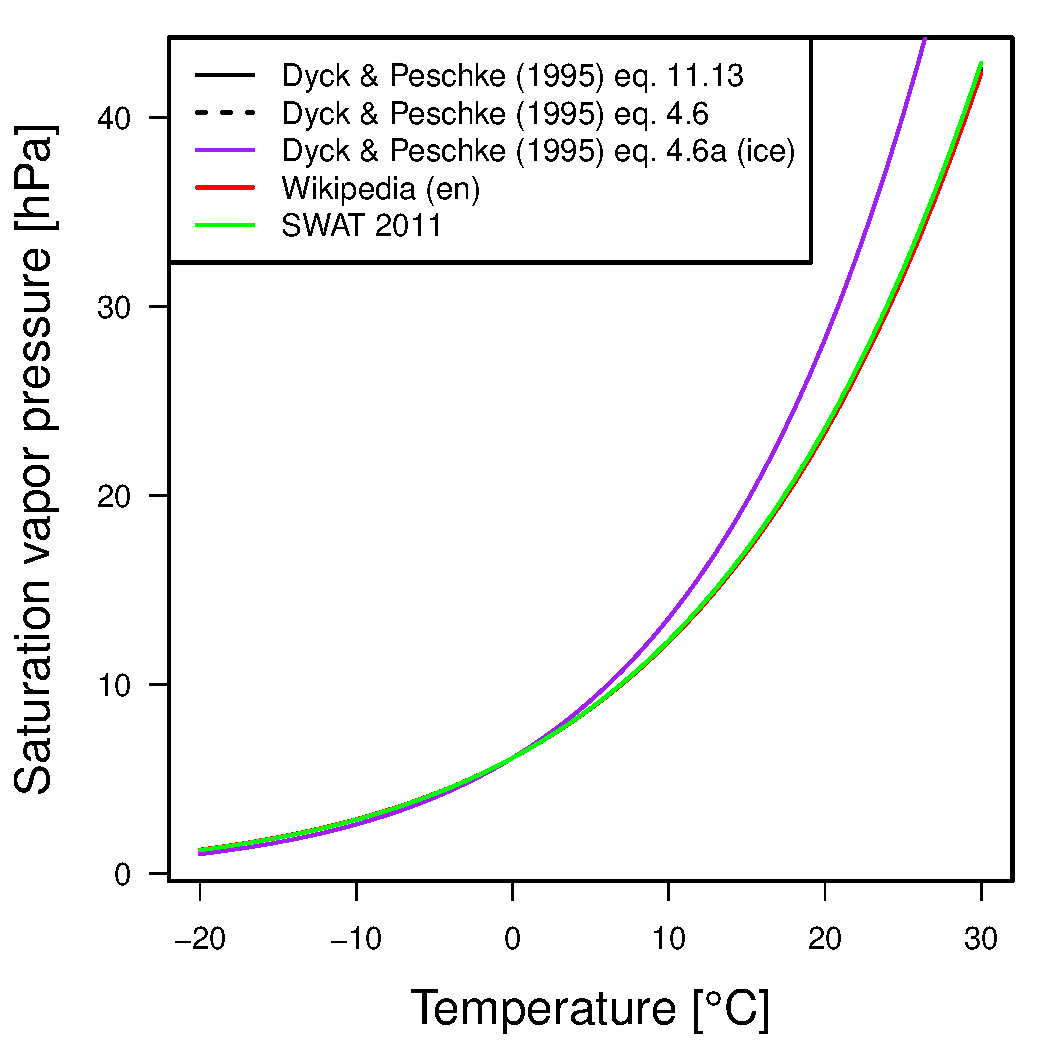
\includegraphics[width=\columnwidth]{\figdir/compare_satVapPress_formulas.ps}
  \caption{Comparison of different approaches for the calculation of saturated water vapor pressure obtained from \citet{Dyck1995, Neitsch2011}, and \url{https://en.wikipedia.org/wiki/Clausius-Clapeyron_relation}. \label{fig:meteo:satVapPress}}
\end{figure}


\subsection{Vapor pressure -- \vaporPressure} \label{sec:meteo:vappress}
As the relative humidity \relHumidity{} (\verb!relhum!) of air is defined as the proportion of actual water vapor pressure \vaporPressure{} to saturated water vapor pressure \satVaporPressure{} (both in [\si{\hecto\pascal}]), the former can be easily derived from measurements of air temperature \airtemp{} (\verb!temp!; in [\si{\degreeCelsius}] to estimate \satVaporPressure{}) and \relHumidity{} in [\si{\percent}]:

\begin{equation} \label{eqn:meteo:vapPress}
\vaporPressure{} = \frac{\satVaporPressure{(\airtemp{})} \cdot \relHumidity{}}{100}
\end{equation}

\noindent
Usage:\\
\verb!vapPress_overWater(temp, relhum)!\\
\verb!vapPress_overIce(temp, relhum)!


\subsection{Vapor pressure deficit -- \vaporPressureDeficit} \label{sec:meteo:vappressdef}
In ECHSE water vapor pressure deficit in [\si{\hecto\pascal}], i.e. $\satVaporPressure{(\airtemp{})} - \vaporPressure{}$ (cf. \secsref{sec:meteo:satvappress} \ref{sec:meteo:vappress}), can by directly computed from air temperature (\airtemp{}, \verb!temp! in [\si{\degreeCelsius}]) and relative humidity (\relHumidity{}, \verb!relhum! in [\si{\percent}]).

\noindent
Usage:\\
\verb!vapPressDeficit_overWater(temp, relhum)!\\
\verb!vapPressDeficit_overIce(temp, relhum)!


\subsection{Slope of the saturation vapor pressure curve -- \slopeSatVapCurve} \label{sec:meteo:slopevappress}
The slope of the saturation vapor pressure temperature curve (\slopeSatVapCurve{} in [\si{\hecto\pascal\per\kelvin}]; in a more general sense also known as \emph{Clausius-Clapeyron} relation) is derived by differentiation of the saturation vapor pressure \satVaporPressure{} with respect to air temperature \airtemp{} (\verb!temp!). \citet{Dyck1995} derived the following equation by differentiation of the \emph{Magnus formula} (cf. \secref{sec:meteo:satvappress}) which is implemented in ECHSE (\airtemp{} in [\si{\degreeCelsius}]):

\begin{equation} \label{eqn:meteo:slopeSatVapCurve}
\slopeSatVapCurve{} = \frac{4098 \cdot \satVaporPressure{(\airtemp{})}}{\left( 273.3 + \airtemp{} \right)^2}
\end{equation}

\noindent
Usage:
\verb!slopeSatVapPress(temp)!\\

Note that herein the temperature dependence of latent heat of evaporation of water is neglected which should, however, be sufficient within the general purpose of evapotranspiration calculation (see Wikipedia for more information: \url{https://en.wikipedia.org/wiki/Clausius-Clapeyron_relation}).


\subsection{Dew point temperature -- \dewpointTemperature} \label{sec:meteo:dewtemp}

TODO


\subsection{Specific humidity -- \specHumidity} \label{sec:meteo:spechum}
Specific humidity (\specHumidity{}, dimensionless) is the ratio of mass of water in a parcel of air to the total mass. \citet{Dyck1995} give the following simplified equation depending on vapor pressure (\vaporPressure{}, \verb!vapPress! in [\si{\hecto\pascal}]; cf. \secref{sec:meteo:vappress}) and air pressure (\airPressure{}, \verb!pressAir! in [\si{\hecto\pascal}]; cf. \secref{sec:meteo:apress}) only:

\begin{equation} \label{eqn:meteo:spechum}
\specHumidity{} = \frac{0.622 \cdot \vaporPressure{}}{\airPressure{} - 0.378 \cdot \vaporPressure{}}
\end{equation}

\noindent
Usage:
\verb!specificHumidity(pressAir, vapPress)!\\


\subsection{Latent heat of water evaporation -- \evapHeatWater} \label{sec:meteo:evapheat}
Latent heat of water evaporation, or heat equivalent of water, (\evapHeatWater{} in [\si{\kilo\joule\per\kilo\gram}]) is a function of temperature (\airtemp{}, \verb!temp! in [\si{\degreeCelsius}]) and can be derived from the following empirical formula \citep{Dyck1995}:

\begin{equation} \label{eqn:meteo:evapheat}
\evapHeatWater{} = 2501 - 2.37 \cdot \airtemp{}
\end{equation}

\noindent
Usage:
\verb!latentHeatEvap(temp)!\\

Note that for sublimation and deposition from and into ice a different formula must be used (not yet included in ECHSE).


\subsection{Psychrometric constant -- \psychroConst} \label{sec:meteo:psychro}
The psychrometric constant (\psychroConst{} in [\si{\hecto\pascal\per\kelvin}]) relates the partial pressure of water in the air to temperature. It depends on atmospheric pressure (\airPressure{}, \verb!airpress! in [\si{\hecto\pascal}]) and heat equivalent of water \evapHeatWater{}, which in turn depends on air temperature (\airtemp{}, \verb!temp! in [\si{\degreeCelsius}]; cf. \secref{sec:meteo:evapheat}), as boundary conditions, and the constants ratio of molecular weight of water vapor to that of dry air and specific heat of air at constant pressure. In summarized form, it can be eventually calculated using the following relation \citep{Dyck1995}:

\begin{equation} \label{eqn:meteo:psychro}
\psychroConst{} = 0.016286 \frac{\airPressure{}}{\evapHeatWater{(\airtemp{})}}
\end{equation}

\noindent
Usage:
\verb!psychroConst(temp, airpress)!\\


\subsection{Mole fraction of water vapor -- \moleFracWaterVap} \label{sec:meteo:molefracvap}
The mole fraction of water vapor is a dimensionless number meaning the amount of water vapor in air. Following the definition from the \emph{International Committee for Weights and Measures CIPM-81/91} its realization in ECHSE is:

\begin{multline}\label{eqn:meteo:molefracvap}
\moleFracWaterVap{} = \relHumidity{} \\ 
(\num{1.00062} + \num{3.14e-08} \cdot \airPressure{} + \num{5.6e-07} \cdot \airtemp{}^2) \\
\frac{\satVaporPressure{(\airtemp{})}}{\airPressure{}}
\end{multline}

\noindent
Usage:\\
\verb!moleFrac_waterVap(airpress,temp,relhum)!\\

Where \relHumidity{}/\verb!relhum! means relative humidity in [\si{\percent}], \airPressure{}/\verb!airpress! is air pressure in [\si{\hecto\pascal}], and \satVaporPressure{} is saturation vapor pressure in [\si{\hecto\pascal}] depending on air temperature (\airtemp{}, \verb!temp! in [\si{\degreeCelsius}]; cf. \secref{sec:meteo:satvappress}). \textbf{Note} that these units are needed for input, internal conversions are applied that are not shown here.


\subsection{Compressibility factor -- \compressibilityFactor} \label{sec:meteo:compressfac}
The compressibility factor (dimensionless) is used to calculate the density of moist air. The ECHSE implementation follows the definition from the \emph{International Committee for Weights and Measures CIPM-81/91} taking into account air pressure (\airPressure{}, \verb!airpress! in [\si{\hecto\pascal}]), temperature (\airtemp{}, \verb!temp! in [\si{\degreeCelsius}]), and relative humidity (\relHumidity{}, \verb!relhum! in [\si{\percent}]) (\textbf{NOTE:} Units shown are needed for input, internal conversions are applied that are not shown here):

\begin{multline}\label{eqn:meteo:compressfac}
\compressibilityFactor{} = 1 - \frac{\airPressure{}}{T_{deg\_K} + \airtemp{}} \\
[a_0 + a_1 t + a_2 t^2 + (b_0 + b_1 t) \moleFracWaterVap{} + (c_0 + c_1 t) \moleFracWaterVap{}^2 ] \\
+ \frac{\airPressure{}^2}{(T_{deg\_K} + \airtemp{})^2} \cdot (d + e \moleFracWaterVap{}^2)
\end{multline}

\noindent
Usage:
\verb!f_compress(airpress,temp,relhum)!\\

\noindent
Where:
\sisetup{
detect-family,
detect-display-math = true
}
\[ a_0 = \SI{1.58123e-06}{\kelvin\per\pascal} \]
\[ a_1 = \SI{-2.9331e-08}{\per\pascal} \]
\[ a_2 = \SI{1.1043e-10}{\per\kelvin\per\pascal} \]
\[ b_0 = \SI{5.707e-06}{\kelvin\per\pascal} \]
\[ b_1 = \SI{-2.051e-08}{\per\pascal} \]
\[ c_0 = \SI{1.9898e-4}{\kelvin\per\pascal} \]
\[ c_1 = \SI{-2.376e-06}{\per\pascal} \]
\[ d = \SI{1.83e-11}{\kelvin\squared\per\pascal\squared} \]
\[ e = \SI{-0.765e-08}{\kelvin\squared\per\pascal\squared} \]

For \moleFracWaterVap{} see \secref{sec:meteo:molefracvap} and for $T_{deg\_K}$ see \secref{sec:meteo:constants}.


\subsection{Density of moist air -- \densityAirMoist} \label{sec:meteo:densairmoist}
To calculate the density of moist air (\densityAirMoist{} in [\si{\kilo\gram\per\cubic\metre}]) the most recent version of the formula from the \emph{International Committee for Weights and Measures (CIPM)}, published and analyzed by \citet{Picard2008}, is incorporated in ECHSE:

\begin{multline}\label{eqn:meteo:densairmoist}
\densityAirMoist{} = \frac{\airPressure{} \cdot \molMassDryAir{}}{\compressibilityFactor{} \cdot \molGasConst \cdot (T_{deg\_K} + \airtemp{})} \\
\left[ 1 - \moleFracWaterVap{} \left( 1 - \frac{\molMassWater{}}{\molMassDryAir{}} \right) \right]
\end{multline}

\noindent
Usage:\\
\verb!densityMoistAir(airpress,temp,relhum)!\\

Air pressure (\airPressure{}, \verb!airpress! in [\si{\hecto\pascal}]), temperature (\airtemp{}, \verb!temp! in [\si{\degreeCelsius}]), and relative humidity (\relHumidity{}, \verb!relhum! in [\si{\percent}]) have to be given. For derivation of \compressibilityFactor{}, and \moleFracWaterVap{} see \secsref{sec:meteo:compressfac}, and \ref{sec:meteo:molefracvap}, respectively. For the constants \molMassDryAir{}, \molMassWater{}, \molGasConst{}, and $T_{deg\_K}$ see \secref{sec:meteo:constants}.


\section{Astronomical quantities}

\subsection{Solar declination -- \solDecl} \label{sec:meteo:soldecl}
Solar declination (\solDecl{} in [\si{\radian}]) is the angle between the rays of the Sun and a plane of the Earth's equator. It varies roughly between \SI{+23.5}{\degree} on June solstice and \SI{-23.5}{\degree} on December solstice caused by the Earth's axial tilt. In ECHSE incorporated is an approximation as used in the SWAT model \citep{Neitsch2011} which should not be used in cases where high accuracy is needed but which is sufficient for estimation of the energy balance (for which \solDecl{} is basically used in ECHSE):

\begin{equation}\label{eqn:meteo:soldecl}
\solDecl{} = \arcsin \left\{ 0.4 \sin \left[ \frac{2 \pi}{365} (\doy{} - 82) \right] \right\}
\end{equation}

\noindent
Usage:
\verb!sol_decl(doy)!\\

Where \doy{} (\verb!doy!) is the current \emph{Julian day} or \emph{day of the year}.


\subsection{Eccentricity correction factor -- \eccCorr} \label{sec:meteo:eccorr}
The eccentricity correction factor \eccCorr{} (dimensionless) accounts for that the Earth's orbit around the Sun is not a perfect circle but slightly elliptical. ECHSE incorporates a simplified formula following the implementation in the SWAT model \citep{Neitsch2011}:

\begin{equation}\label{eqn:meteo:eccorr}
\eccCorr{} = \left( \frac{r_0}{r} \right)^2 = 1 + 0.033 \cos \left(\frac{2 \pi \doy}{365} \right)
\end{equation}

\noindent
Usage:
\verb!eccorr(doy)!\\

Where $r_0$ is the average and $r$ the distance between Earth and Sun for any day of the year, and \doy{} (\verb!doy!) is the current \emph{Julian day} or \emph{day of the year}. For simplification, day \num{366} at leap years is set to \num{365} as otherwise the above formula would not give a reasonable value. It should thus not be used in cases where high accuracy is needed.


\subsection{Daylight time factor -- \dayTimeFac} \label{sec:meteo:daytimefac}
The daylight time factor \dayTimeFac{} is the approximate hour angle in [\si{\radian}] of sunrise and sunset at a specific location at given latitude (\lat{}, \verb!lat! in [\si{\degree}]) on a specific day of the year (\doy{}, \verb!doy!, dimensionless) following equation 25 of FAO's \emph{Guidelines for computing crop water requirements, Chapter 3: Meteorological data} (\url{http://www.fao.org/docrep/X0490E/x0490e07.htm#calculation\%20procedures}):

\begin{equation}\label{eqn:meteo:daytimefac}
\dayTimeFac{} = \arccos \left[ -tan(\solDecl{(\doy)}) tan(\lat{}) \right]
\end{equation}

\noindent
Usage:
\verb!dayTime_fac(doy, lat)!\\

Where \solDecl{} is the solar declination in [\si{\radian}], cf. \secref{sec:meteo:soldecl}. \textbf{Note} that units shown are needed for input, internal conversions are applied.


\subsection{Extraterrestrial radiation -- \radExtraterr} \label{sec:meteo:radex}
Extraterrestrial radiation \radExtraterr{} in [\si{\watt\per\metre\squared}] is the radiation coming from the Sun and hitting the top of the Earth's atmosphere over a given day of the year (\doy{}, \verb!doy!, dimensionless) at a location of given latitude (\lat{}, \verb!lat! in [\si{\degree}]).

On a \textbf{daily} basis it is calculated by integrating incoming solar radiation from sunrise to sunset. See, e.g., \citet{Neitsch2011} or any textbook for a deviation resulting in the following formula (respect units!):

\begin{multline}\label{eqn:meteo:radex_d}
\radExtraterrDaily{} = \frac{1}{\pi} \cdot \solarConstant{} \cdot \eccCorr{} \\
\left[ \dayTimeFac{} \cdot \sin(\solDecl{}) \cdot \sin(\lat{}) + \cos(\solDecl{}) \cdot \cos(\lat{}) \cdot \sin(\dayTimeFac{}) \right]
\end{multline}

\noindent
Usage:
\verb!rad_extraterr_daily(doy, lat)!\\

For \solarConstant{} see \secref{sec:meteo:constants} and for \eccCorr{}, \dayTimeFac{}, and \solDecl{} see \secsref{sec:meteo:eccorr}, \ref{sec:meteo:daytimefac}, and \ref{eqn:meteo:soldecl}, respectively.

To obtain \textbf{hourly} values the solar time angles at the beginning and the end of the hour of interest have to be respected. Furthermore, a correction for the local time zone has to be applied. Following equations 28 to 33 of FAO's \emph{Guidelines for computing crop water requirements, Chapter 3: Meteorological data} (\url{http://www.fao.org/docrep/X0490E/x0490e07.htm#calculation\%20procedures}) the subsequent relations are implemented in ECHSE:

\noindent
Calculation of the solar time angle $\omega_{mid}$ in [\si{\radian}] at the midpoint of the desired hour of the day $h$ (\verb!hour!, integer number):

\begin{multline}\label{eqn:meteo:radex_h:w_mid}
\omega_{mid} = \frac{\pi}{12} \\
\left\{ \left[ (h + 0.5) + 0.06667 \cdot (L_z - L_m) + S_c \right] - 12 \right\}
\end{multline}

\noindent
with $L_m$ (\verb!L_m!) being the longitutde of the location of interest in decimal degrees west of Greenwich (e.g. Greenwich: \SI{0}{\degree}, New York: \SI{75}{\degree}, Berlin: \SI{346.5}{\degree}), $L_z$ the longitude of the center of the local time zone which is computed internally from the deviation of the local time zone from universal time (UTC) which has to be given as input (\verb!utc_add!, integer value of [\numrange[range-phrase=..]{-12}{14}])\footnote{\textbf{Note} that the value might change over the year in case of \emph{daylight saving time} and thus should be given as time series input rather than just being a fixed parameter!}, and $S_c$ a seasonal correction factor that is computed internally. Using that the solar time angles at begin and end of the hour of interest can be calculated:

\begin{equation}\label{eqn:meteo:radex_h:w_ini_end}
\begin{split}
\omega_{ini} &= \omega_{mid} - \frac{\pi}{24},\\
\omega_{end} &= \omega_{mid} + \frac{\pi}{24}
\end{split}
\end{equation}

\noindent
where, of course, radiation is zero if $\omega_{mid} < -\dayTimeFac{}$ or $\omega_{mid} > \dayTimeFac{}$ (for \dayTimeFac{} see \secref{sec:meteo:daytimefac}), i.e. if the Sun is not shining (note from \eqnref{eqn:meteo:radex_h:w_mid} that the accuracy is $\pm$ half an hour). Eventually, analog to \radExtraterrDaily{}, hourly values of \radExtraterr{} can be obtained:

\begin{multline}\label{eqn:meteo:radex_h}
\radExtraterrHourly{} = \frac{1}{\pi} \cdot \solarConstant{} \cdot \eccCorr{}\\
\big[ (\omega_{end}-\omega_{ini}) \cdot \sin(\solDecl{}) \cdot \sin(\lat{})\\
+ \cos(\solDecl{}) \cdot \cos(\lat{}) \cdot (\sin(\omega_{end})-\sin(\omega_{ini})) \big]
\end{multline}

\noindent
Usage:
\begin{verbatim}
rad_extraterr_hourly(doy,lat,hour,
utc_add,L_m)
\end{verbatim}

\figref{fig:meteo:radex_h} shows example outputs of hourly extraterrestrial radiation computed with \eqnsref{eqn:meteo:radex_h:w_mid} to \ref{eqn:meteo:radex_h} over four specific days of year for Berlin taking \emph{daylight saving time} into account.

\begin{figure}
  \centering
  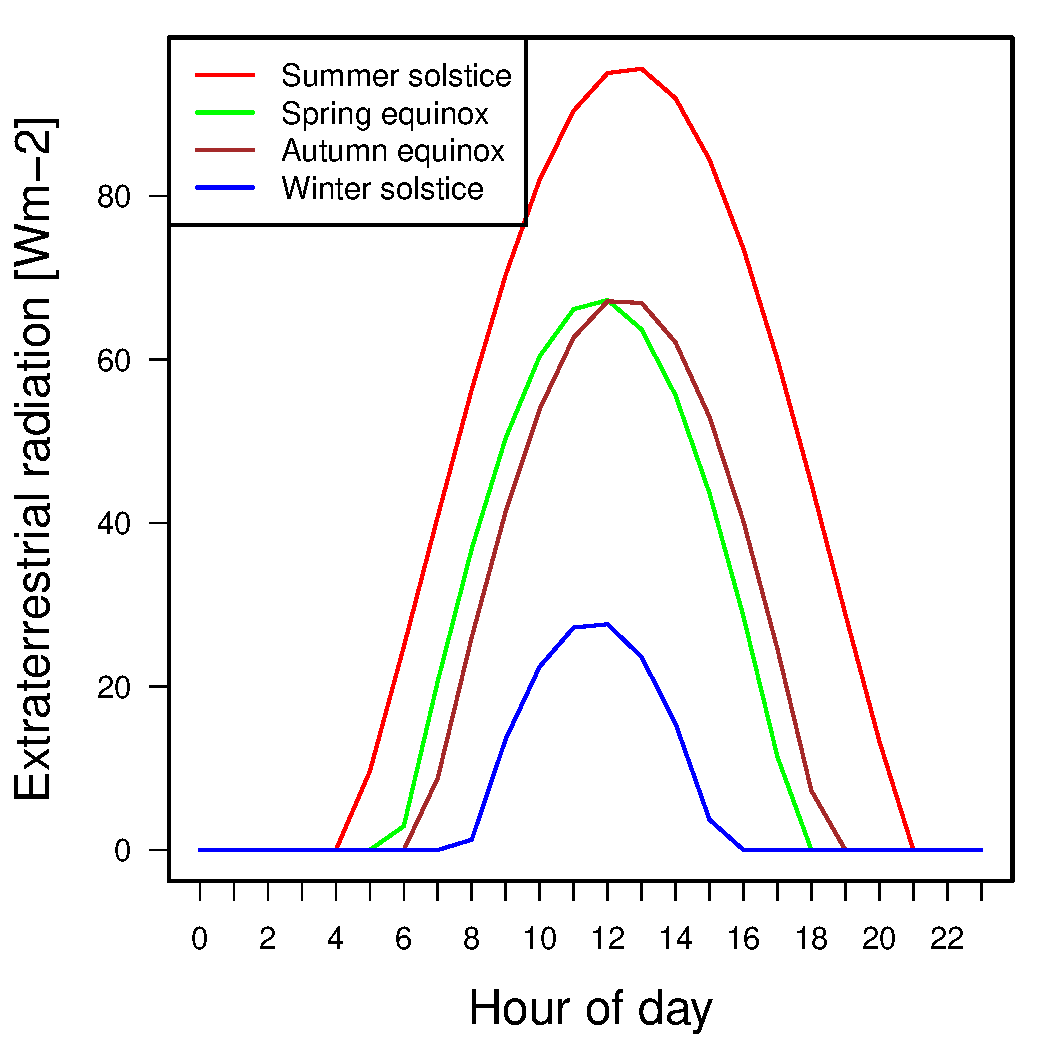
\includegraphics[width=\columnwidth]{\figdir/test_radex_hourly.ps}
  \caption{Hourly extraterrestrial radiation computed using \eqnsref{eqn:meteo:radex_h:w_mid} to \ref{eqn:meteo:radex_h} over four specific days of year (line colors, see legend) for Berlin taking \emph{daylight saving time} into account.\label{fig:meteo:radex_h}}
\end{figure}

\textbf{Note} that units shown are needed for input, internal conversions are applied.


\section{Energy budget}

\subsection{Incoming short-wave radiation -- \radShortwaveIn} \label{sec:meteo:radshort}
Shortwave radiation received by the surface is typically lower than \emph{extraterrestrial radiation} discussed in \secref{sec:meteo:radex} due to processes of absorption, scattering, and reflection in the Earth's atmosphere. It is typically measured at weather stations but can be calculated if no observations are available using the relation of {\AA}ngström (see textbooks, e.g. \citet{Maidment1993}):

\begin{equation}\label{eqn:meteo:radshort}
\radShortwaveIn{} = \left( a_s + b_s \frac{n}{N} \right) \radExtraterr{}
\end{equation}

\noindent
Usage:
\begin{verbatim}
calc_glorad(radex,sundur,cloud,lat
doy,radex_a,radex_b)
\end{verbatim}

\radShortwaveIn{} is computed in [\si{\watt\per\metre\squared}], \radExtraterr{} is extraterrestrial radiation (\verb!radex! in [\si{\watt\per\metre\squared}], cf. \secref{sec:meteo:radex}), $\frac{n}{N}$ is the fraction of measured (\verb!sundur!) to maximum possible sunshine duration, the latter calculated internally from \dayTimeFac{} (cf. \secref{sec:meteo:daytimefac}) which needs the current day of year \verb!doy! and the latitude \verb!lat! of the location of interest in [\si{\degree}] as inputs:

\begin{equation}\label{eqn:meteo:radshort:sundur}
N = \dayTimeFac{} \frac{24}{\pi}
\end{equation}

$a_s$ (\verb!radex_a!) and $b_s$ (\verb!radex_b!) are the {\AA}ngström coefficients. The latter define the fraction of \radExtraterr{} that reaches the surface on completely cloudy ($a_s$) and days of clear sky ($a_s + b_s$), respectively. They can be estimated from measured values (e.g. from a near-by station) or derived from look-up tables (for average climates \citet{Maidment1993} suggests $a_s = \num{0.25}$ and $b_s = \num{0.50}$). Note that measurements of cloudiness (\verb!cloud!) as input to estimate $\frac{n}{N}$ are not yet supported (although the function interface includes it) but planned for the future.

\textbf{Note} that units shown are needed for input, internal conversions are applied.


\subsection{Maximum (clear-sky) incoming short-wave radiation -- \radShortwaveInClearsky} \label{sec:meteo:radshortmax}
The maximum possible incoming short-wave radiation in case of clear sky (\radShortwaveInClearsky{} in [\si{\watt\per\metre\squared}]) is calculated analogue to \radShortwaveIn{} (cf. \secref{sec:meteo:radshort}) assuming full sunshine duration and thus $\frac{n}{N} = \num{1}$:

\begin{equation}\label{eqn:meteo:radshortmax}
\radShortwaveInClearsky{} = \left( a_s + b_s \right) \radExtraterr{}
\end{equation}

\noindent
Usage:\\
\verb!calc_glorad_max(radex,radex_a,radex_b)!


\subsection{Net emissivity -- \emissivity} \label{sec:meteo:emiss}
Emissivity characterizes the effectiveness of a surface in emitting energy as thermal long-wave radiation. In this case the net emissivity between the Earth's surface and the atmosphere is sought which depends on the amount of water in the air and can thus be empirically related to the water vapor pressure (\vaporPressure{} in [\si{\hecto\pascal}]; cf. \secref{sec:meteo:vappress}) \citep{Maidment1993}:

\begin{equation}\label{eqn:meteo:emis_1}
\emissivity{} = a_e + b_e \sqrt{\vaporPressure{}}
\end{equation}

\noindent
Usage:
\verb!net_emiss(temp,relhum,a,b)!\\

The parameters $a_e$ and $b_e$ are in the range of \num{0.34} to \num{0.44} and \num{-0.25} to \num{-0.14}, respectively, whereas for average conditions the values $a_e = \num{0.34}$ and $b_e = \num{-0.14}$ are typically used \citep{Maidment1993}.

If no measurements of relative humidity (\relHumidity{}, \verb!relhum! in [\si{\percent}]) for estimation of \vaporPressure{} are available, \emissivity{} can be as well estimated solely from temperature (\airtemp{}, \verb!temp! in [\si{\degreeCelsius}]) \citep{Maidment1993}:

\begin{equation}\label{eqn:meteo:emis_2}
\emissivity{} = -0.02 + 0.261 \exp(\num{-7.77e-4} \airtemp{}^2)
\end{equation}

\textbf{Note} that units shown are needed for input, internal conversions are applied.


\subsection{Cloudiness correction factor -- \cloudCorrFac} \label{sec:meteo:cloudcorr}
The cloudiness correction factor (\cloudCorrFac{}, dimensionless) is an empirical factor to correct calculations of long-wave radiation at the Earth's surface for cloud cover (cf. \secref{sec:meteo:radnetlong}). It can be calculated from the ratio of actual short-wave radiation (\radShortwaveIn{}, \verb!glorad! in [\si{\watt\per\metre\squared}]) to maximum short-wave radiation at clear sky (\radShortwaveInClearsky{}, \verb!glorad_max! in [\si{\watt\per\metre\squared}]) \citep{Maidment1993}:

\begin{equation}\label{eqn:meteo:cloudcorr}
\cloudCorrFac{} = a_c \frac{\radShortwaveIn{}}{\radShortwaveInClearsky{}} + b_c
\end{equation}

\noindent
Usage:
\verb!f_cloud(glorad,glorad_max,a,b)!\\

The long-wave radiation coefficients for clear skies $a_c$ and $b_c$ should be estimated from local radiation measurements. However, \citet{Maidment1993} suggests $a_c = \num{1.35}$ and $b_c = \num{-0.35}$ for arid areas, and $a_c = \num{1.00}$ and $b_c = \num{0.00}$ for humid areas.


\subsection{Incoming net long-wave radiation -- \netRadiationLong} \label{sec:meteo:radnetlong}
Applying the \emph{law of Stefan-Boltzmann} the incoming net long-wave radiation at the Earth's surface (\netRadiationLong{} in [\si{\watt\per\metre\squared}]) can be calculated from \citep{Maidment1993}:

\begin{equation}\label{eqn:meteo:radnetlong}
\netRadiationLong{} = - \cloudCorrFac{} \emissivity{} \stefanBoltzmann{} (\airtemp{} + T_{deg\_K})^4
\end{equation}

\noindent
Usage:
\begin{verbatim}
net_longrad(temp,relhum,glorad,
glorad_max,emis_a,emis_b,
fcorr_a,fcorr_b)
\end{verbatim}

\netRadiationLong{} is defined positive in direction to the ground, i.e. negative values indicate a net loss, positive values net gain of energy at the Earth's surface. For \cloudCorrFac{} (including the radiation coefficients \verb!fcorr_a! and \verb!facorr_b!) and \emissivity{} (including the emissivity parameter \verb!emis_a! and \verb!emis_b!) see \secsref{sec:meteo:cloudcorr} and \ref{sec:meteo:emiss}, respectively. For \stefanBoltzmann{} and $T_{deg\_K}$ see \secref{sec:meteo:constants}. \airtemp{} (\verb!temp!) is the air temperature in [\si{\degreeCelsius}].


\subsection{Incoming net radiation -- \netRadiation} \label{sec:meteo:radnet}
The total incoming net radiation (\netRadiation{} in [\si{\watt\per\metre\squared}]) is the sum of incoming net long-wave radiation (\netRadiationLong{}, cf. \secref{sec:meteo:radnetlong}) and incoming net short-wave radiation, i.e. the amount of incoming short-wave radiation \radShortwaveIn{} (cf. \secref{sec:meteo:radshort}) absorbed by the ground \citep{Maidment1993}:

\begin{equation}\label{eqn:meteo:radnet}
\netRadiation{} = (1 - \albedo{}) \radShortwaveIn{} + \netRadiationLong{}
\end{equation}

\noindent
Usage:
\begin{verbatim}
net_rad(temp,relhum,glorad,glorad_max,
emis_a,emis_b,fcorr_a,fcorr_b)
\end{verbatim}

Albedo (\albedo{}) is a quantity depending on land cover. It can be derived from local measurements of the radiation balance or from look-up tables. As it might change over the year it is advised to supply it as time series input rather than as a fixed parameter.


\subsection{Soil heat flux -- \heatfluxSoil} \label{sec:meteo:soilflux}
Soil heat flux (\heatfluxSoil{} in [\si{\watt\per\metre\squared}]) is the conduction of heat through the soil. It varies over the day and depends on land-cover conditions. According to textbooks it can be neglected over daily time scales which is generally done in the context of hydrological applications. At sub-daily application, however, it cannot be neglected and is typically defined as a fraction of net radiation \netRadiation{} (\verb!net_rad! in [\si{\watt\per\metre\squared}]). In equations 45 and 46 of FAO's \emph{Guidelines for computing crop water requirements, Chapter 3: Meteorological data} (\url{http://www.fao.org/docrep/X0490E/x0490e07.htm#calculation\%20procedures}) it is suggested to take \SI{10}{\percent} during daylight periods and \SI{50}{\percent} during nighttime, \citet{Shuttleworth1985} arbitrarily set it to \SI{20}{\percent}, and \citet{Guentner2002} identified in a literature study \SI{20}{\percent} during daytime and \SI{70}{\percent} for nighttime periods as appropriate for (semi-)arid conditions with sparse vegetation cover. These approaches are implemented in ECHSE, taking the fraction of \netRadiation{} over daytime (\verb!f_day!) and nighttime (\verb!f_night!), a flag specifying if, at the current time step, it is day ($\verb!daynight! = 1$) or nighttime ($\verb!daynight! = 0$), and the current time step length (\verb!delta_t! in [\si{\second}]) to differentiate between the two approaches as inputs.\\

\noindent
Usage:
\begin{verbatim}
soil_heatflux(net_rad,f_day,f_night,
daynight,delta_t)
\end{verbatim}

For monthly time scales further approaches exist depending on temperature, soil heat conductivity, and effective soil depth (cf. \citet{Maidment1993} or \url{http://www.fao.org/docrep/X0490E/x0490e07.htm#calculation\%20procedures}).

\include{chapters/part_processes/reservoirStorage/reservoirStorage}

%%%%%%%%%%%%%%%%%%%%%%%%%%%%%%%%%%%%%%%%%%%%%%%%%%%%%%%%%%
%%%%%%%%%%%%%%%%%%%%% LISTS %%%%%%%%%%%%%%%%%%%%%%%%%%%%%%
%%%%%%%%%%%%%%%%%%%%%%%%%%%%%%%%%%%%%%%%%%%%%%%%%%%%%%%%%%
\clearpage
\fancyhead[LE,RO]{\bfseries\thepage}
\fancyhead[RE]{\bfseries List of figures}
\fancyhead[LO]{\bfseries List of figures}
\addcontentsline{toc}{chapter}{List of figures}
\listoffigures

\clearpage
\fancyhead[LE,RO]{\bfseries\thepage}
\fancyhead[RE]{\bfseries List of tables}
\fancyhead[LO]{\bfseries List of tables}
\addcontentsline{toc}{chapter}{List of tables}
\listoftables

%%%%%%%%%%%%%%%%%%%%%%%%%%%%%%%%%%%%%%%%%%%%%%%%%%%%%%%%%%
%%%%%%%%%%%%%%%%%%%%% BIBLIOGRAPHY %%%%%%%%%%%%%%%%%%%%%%%
%%%%%%%%%%%%%%%%%%%%%%%%%%%%%%%%%%%%%%%%%%%%%%%%%%%%%%%%%%
\clearpage
\fancyhead[LE,RO]{\bfseries\thepage}
\fancyhead[RE]{\bfseries Bibliography}
\fancyhead[LO]{}
\addcontentsline{toc}{chapter}{Bibliography}
\bibliographystyle{../_common/elsarticle-harv}
\bibliography{../_common/bib_hydrologicalModeling}

%%%%%%%%%%%%%%%%%%%%%%%%%%%%%%%%%%%%%%%%%%%%%%%%%%%%%%%%%%
%%%%%%%%%%%%%%%%%%%%% THE APPENDIX %%%%%%%%%%%%%%%%%%%%%%%
%%%%%%%%%%%%%%%%%%%%%%%%%%%%%%%%%%%%%%%%%%%%%%%%%%%%%%%%%%

\chaptermark{A}
\clearpage
\fancyhead[LE,RO]{\bfseries\thepage}
\fancyhead[RE]{\bfseries Appendix}
\fancyhead[LO]{}
\addcontentsline{toc}{chapter}{Appendix}
\appendix
%\input{appendix/dummy/dummy}

\end{document}
